\documentclass{article}
\usepackage{authblk}
\usepackage{tgpagella}
\usepackage{tikz}
\usetikzlibrary{decorations.pathreplacing}
\usepackage[dvips,letterpaper,margin=1in]{geometry}

% -===============                                    ===============%
% -===============                                    ===============%
% -===============                                    ===============%
%                           PACKAGES                                 %
% -===============                                    ===============%
% -===============                                    ===============%
% -===============                                    ===============%

\usepackage{silence}
\WarningFilter*{hyperref}{Token not allowed in a PDF string}
\WarningsOff[caption]
\usepackage[utf8]{inputenc}
\usepackage[T1]{fontenc}
\usepackage{tabularx}
\usepackage{hyperref}
\usepackage{lipsum}
\usepackage{url}
\usepackage{placeins}
\usepackage{booktabs}
\usepackage{soul}
\usepackage{amsfonts}
\usepackage{nicefrac}
\usepackage{microtype}
\usepackage{natbib}
\usepackage{proba}
\usepackage{wrapfig}
\usepackage{caption}
\usepackage{amssymb}
\usepackage{pifont}
\newcommand{\cmark}{\ding{51}}
\newcommand{\xmark}{\ding{55}}
\usepackage{subcaption}
\usepackage{float}
\usepackage{rotating}
\usepackage{etoolbox}
\usepackage{xparse}
\usepackage{grffile}
\usepackage{amsmath}
\usepackage{xspace}
\usepackage{euscript}
\usepackage{enumitem}
\usepackage{mathtools}
\usepackage{tikz}
\usepackage{tablefootnote}
\usepackage[flushleft]{threeparttable}
\usepackage{multirow}
\usepackage[title]{appendix}
\usepackage{arydshln}
\usepackage{array, booktabs}
\usepackage{comment}
\usepackage{graphicx}
\usepackage{adjustbox}
\usepackage{dsfont}
\usepackage{amsmath,amsthm}
\usepackage{balance}
\usepackage{multicol}
\usepackage{xcolor}
\usepackage{nameref}
\usepackage{pdfpages}
\usepackage{braket}
\usepackage[normalem]{ulem}
\usepackage{bbding}
\usepackage[capitalise,noabbrev]{cleveref}
\usepackage{tcolorbox}
\usepackage{xfrac}
\usepackage[usestackEOL]{stackengine}
\usepackage{indentfirst}
\usepackage{csquotes}
\usepackage{pgf}
\usepackage{varwidth}
\usepackage{verbatimbox}
\usepackage{verbatim}
\usepackage{bm}
\usepackage[colorinlistoftodos,prependcaption,textsize=small]{todonotes}

\usepackage{empheq}
\definecolor{myblue}{rgb}{.8, .8, 1}
\newcommand*\mybluebox[1]{%
\colorbox{myblue}{\hspace{1em}#1\hspace{1em}}}

% -===============                                    ===============%
% -===============                                    ===============%
% -===============                                    ===============%
%                           CAPTION SETTINGS                         %
% -===============                                    ===============%
% -===============                                    ===============%
% -===============                                    ===============%

\captionsetup{font=small}
\captionsetup[sub]{font=small}
\captionsetup[subfigure]{labelformat = parens, labelsep = space, font = small}
\newcommand{\figleft}{{\em (Left)}}
\newcommand{\figcenter}{{\em (Center)}}
\newcommand{\figright}{{\em (Right)}}
\newcommand{\figtop}{{\em (Top)}}
\newcommand{\figbottom}{{\em (Bottom)}}
\newcommand{\captiona}{{\em (a)}}
\newcommand{\captionb}{{\em (b)}}
\newcommand{\captionc}{{\em (c)}}
\newcommand{\captiond}{{\em (d)}}

% -===============                                    ===============%
% -===============                                    ===============%
% -===============                                    ===============%
%                         COLOR MACROS                               %
% -===============                                    ===============%
% -===============                                    ===============%
% -===============                                    ===============%

\definecolor{pastelblue}{RGB}{76,113,175}
\definecolor{pastelgreen}{RGB}{144,238,144}
\definecolor{pastelred}{RGB}{196,78,82}
\definecolor{pastelgrey}{RGB}{230,230,230}
\definecolor{pastelbeige}{RGB}{243,236,221}
\definecolor{pastelpurple}{RGB}{154,139,192}
\definecolor{salmon}{RGB}{250, 128, 114}
\definecolor{darkgreen}{rgb}{0,0.6,0}
\definecolor{darkred}{rgb}{0.5,0,0}
\definecolor{verylightgreen}{HTML}{F6FFF9}
\definecolor{verylightred}{HTML}{FFF4F3}
\definecolor{verylightgray}{HTML}{F4F6F6}
\definecolor{babyblueeyes}{rgb}{0.63, 0.79, 0.95}
\definecolor{lightpink}{rgb}{1.00, 0.714, 0.757}


% -===============                                    ===============%
% -===============                                    ===============%
% -===============                                    ===============%
%                           TIKZ MACROS                              %
% -===============                                    ===============%
% -===============                                    ===============%
% -===============                                    ===============%
\usepackage{tikzpeople}
\usetikzlibrary{shapes,decorations,arrows,calc,arrows.meta,fit,positioning}

\tikzset{
    -Latex,auto,node distance =1 cm and 1 cm,semithick,
    state/.style ={ellipse, draw, minimum width = 0.7 cm},
    point/.style = {circle, draw, inner sep=0.04cm,fill,node contents={}},
    bidirected/.style={Latex-Latex,dashed},
    el/.style = {inner sep=2pt, align=left, sloped}
}

% Warning symbol
\newcommand\Warning{%
 \makebox[1.4em][c]{%
 \makebox[0pt][c]{\raisebox{.1em}{\small!}}%
 \makebox[0pt][c]{\color{red}\Large$\bigtriangleup$}}}%

% Text box

\newcommand{\centertikztextbox}[2]{{
\begin{tikzpicture}
\node[draw, align=center,fill=#1,thick](3) at (0,0) { 
\begin{varwidth}{0.9\linewidth}
#2
\end{varwidth}
};
\end{tikzpicture}
}
}

\newcommand{\tikztextbox}[2]{{
\begin{flushleft}
\begin{tikzpicture}
\node[draw, align=left,fill=#1,thick](3) at (0,0) { 
\begin{varwidth}{0.9\linewidth}
#2
\end{varwidth}
};
\end{tikzpicture}
\end{flushleft}
}
}
% Dashed version
\newcommand{\dashedtikztextbox}[3]{{
\begin{flushleft}
\begin{tikzpicture}
\hspace{#2}
\node[draw, align=left,fill=#1, thick, dashed](3) at (0,0) { 
\begin{varwidth}{0.9\linewidth}
#3
\end{varwidth}
};
\end{tikzpicture}
\end{flushleft}
}
}

% Arrow: [ style arguments, eat up, eat down, move right ]
\newcommand{\tikzarrow}[4]{{
\vspace{-#2}
\begin{flushleft}
\begin{tikzpicture}
\hspace{#4}
\node[align=left](1) at (0,0) { 
\begin{varwidth}{0.9\linewidth}
\end{varwidth}
};
\node[align=left](2) at (0,-1.5) { 
\begin{varwidth}{0.9\linewidth}
\end{varwidth}
};
\path[#1,thick] (1) edge (2);
\end{tikzpicture}
\end{flushleft}
\vspace{-#3}
}
}

%Green check
\newcommand{\greencheck}{}%
\DeclareRobustCommand{\greencheck}{%
  \tikz\fill[scale=0.5, color=pastelgreen]
  (0,.35) -- (.25,0) -- (1,.7) -- (.25,.15) -- cycle;
  
 
% This is how you draw a graph in text:
\usetikzlibrary{shapes.misc}
\newcommand*{\graphdraw}{{\scriptsize
		\tikz[scale=0.1]{
			%%% edges
			\draw[thin] (2,0) -- (0,0) -- (0,2) -- (2,2);
			%% vertices
			\draw[fill=blue,draw=blue] (0,0) circle (12pt);
			\draw[fill=red,draw=red] (0,2) circle (12pt);
			\draw[fill=darkgreen,draw=darkgreen] (2,2) circle (12pt);
			\draw[fill=blue,draw=blue] (2,0) circle (12pt);
		}
}}}


% -===============                                    ===============%
% -===============                                    ===============%
% -===============                                    ===============%
%                         THEOREM ENVIRONMENTS                       %
% -===============                                    ===============%
% -===============                                    ===============%
% -===============                                    ===============%

\newtheorem{theorem}{Theorem}
\newtheorem{assumption}{Assumption}
\newtheorem{axiom}{Axiom}
\newtheorem{case}{Case}
\newtheorem{claim}{Claim}
\newtheorem{conclusion}{Conclusion}
\newtheorem{condition}{Condition}
\newtheorem{conjecture}{Conjecture}
\newtheorem{corollary}{Corollary}
\newtheorem{criterion}{Criterion}
\newtheorem{definition}{Definition}
\newtheorem{exercise}{Exercise}
\newtheorem{example}{Example}
\newtheorem{lemma}{Lemma}
\newtheorem{notation}{Notation}
\newtheorem{problem}{Problem}
\newtheorem{proposition}{Proposition}
\newtheorem{property}{Property}
\newtheorem{remark}{Remark}
\newtheorem{solution}{Solution}
\newtheorem{summary}{Summary}
\newtheorem{motivation}{Motivation}
\newtheorem{query}{Query}
\newtheorem{observation}{Observation}
\newtheorem{question}{Question}
% Let cleveref and thmtools work together
\makeatletter
\def\thmt@refnamewithcomma #1#2#3,#4,#5\@nil{%
	\@xa\def\csname\thmt@envname #1utorefname\endcsname{#3}%
	\ifcsname #2refname\endcsname
	\csname #2refname\expandafter\endcsname\expandafter{\thmt@envname}{#3}{#4}%
	\fi}
\makeatother
\Crefname{conjecture}{Conjecture}{Conjectures}
\Crefname{definition}{Definition}{Definitions}
\Crefname{observation}{Observation}{Observations}
\Crefname{assumption}{Assumption}{Assumptions}
\Crefname{axiom}{Axiom}{Axioms}
\Crefname{case}{Case}{Cases}
\Crefname{claim}{Claim}{Claims}
\Crefname{conclusion}{Conclusion}{Conclusions}
\Crefname{condition}{Condition}{Conditions}
\Crefname{criterion}{Criterion}{Criteria}
\Crefname{exercise}{Exercise}{Exercises}
\Crefname{example}{Example}{Examples}
\Crefname{notation}{Notation}{Notations}
\Crefname{problem}{Problem}{Problems}
\Crefname{property}{Property}{Properties}
\Crefname{remark}{Remark}{Remarks}
\Crefname{solution}{Solution}{Solutions}
\Crefname{summary}{Summary}{Summaries}
\Crefname{motivation}{Motivation}{Motivations}
\Crefname{query}{Query}{Queries}
\Crefname{question}{Question}{Questions}
% -===============                                    ===============%
% -===============                                    ===============%
% -===============                                    ===============%
%                           MATH MACROS                              %
% -===============                                    ===============%
% -===============                                    ===============%
% -===============                                    ===============%
\newcommand{\mathcolorbox}[2]{\colorbox{#1}{$\displaystyle #2$}}
\newcommand{\one}{\mathds{1}}
\newcommand{\negquad}{\mkern-18mu}
\newcommand{\red}[1]{{\color{red} #1}}
\DeclareMathOperator*{\argmin}{argmin}
\DeclareMathOperator*{\argmax}{argmax}
\newcommand*\dbar[1]{\overline{\overline{\lower0.2ex\hbox{$#1$}}}}
\newcommand{\supp}{\text{supp\xspace}}
\DeclareMathOperator{\Tr}{Tr}
\newcommand{\dom}{\text{dom}}
\newcommand{\ran}{\text{ran}}
\newcommand{\setsize}[1]{\mid \! #1 \! \mid}
\def\th{^{\text{th}}}
%Stats macros:
\newcommand{\KL}{D_{\mathrm{KL}}}
\newcommand{\pr}{P}
\newcommand{\Exp}{\mathds{E}}
\newcommand{\eqdist}{\stackrel{d}{=}}
\newcommand{\eqas}{\stackrel{\text{a.s.}}{=}}
\newcommand{\standarderror}{\mathrm{SE}}
\newcommand{\indep}{\perp\!\!\!\perp}
%Causality macros
\newcommand{\doop}{\text{do}}
\newcommand{\Parents}{\text{Pa}}
\newcommand{\parents}{\text{pa}}
%Graph macros
\newcommand{\iso}{\cong}
\newcommand{\notiso}{\not cong}
\newcommand{\aut}[1]{\text{Aut}(#1)}
%Machine learning macros:
\newcommand{\lr}{\alpha}
\newcommand{\reg}{\lambda}
\newcommand{\lf}{\mathcal{L}}
\newcommand{\sigmoid}{\sigma}
\newcommand{\softplus}{\zeta}
\newcommand{\relu}{\text{ReLU}}
%Font macros
\def\cA{{\mathcal{A}}}
\def\cB{{\mathcal{B}}}
\def\cC{{\mathcal{C}}}
\def\cD{{\mathcal{D}}}
\def\cE{{\mathcal{E}}}
\def\cF{{\mathcal{F}}}
\def\cG{{\mathcal{G}}}
\def\cH{{\mathcal{H}}}
\def\cI{{\mathcal{I}}}
\def\cJ{{\mathcal{J}}}
\def\cK{{\mathcal{K}}}
\def\cL{{\mathcal{L}}}
\def\cM{{\mathcal{M}}}
\def\cN{{\mathcal{N}}}
\def\cO{{\mathcal{O}}}
\def\cP{{\mathcal{P}}}
\def\cQ{{\mathcal{Q}}}
\def\cR{{\mathcal{R}}}
\def\cS{{\mathcal{S}}}
\def\cT{{\mathcal{T}}}
\def\cU{{\mathcal{U}}}
\def\cV{{\mathcal{V}}}
\def\cW{{\mathcal{W}}}
\def\cX{{\mathcal{X}}}
\def\cY{{\mathcal{Y}}}
\def\cZ{{\mathcal{Z}}}
\def\bA{{\bm{A}}}
\def\bB{{\bm{B}}}
\def\bC{{\bm{C}}}
\def\bD{{\bm{D}}}
\def\bE{{\bm{E}}}
\def\bF{{\bm{F}}}
\def\bG{{\bm{G}}}
\def\bH{{\bm{H}}}
\def\bI{{\bm{I}}}
\def\bJ{{\bm{J}}}
\def\bK{{\bm{K}}}
\def\bL{{\bm{L}}}
\def\bM{{\bm{M}}}
\def\bN{{\bm{N}}}
\def\bO{{\bm{O}}}
\def\bP{{\bm{P}}}
\def\bQ{{\bm{Q}}}
\def\bR{{\bm{R}}}
\def\bS{{\bm{S}}}
\def\bT{{\bm{T}}}
\def\bU{{\bm{U}}}
\def\bV{{\bm{V}}}
\def\bW{{\bm{W}}}
\def\bX{{\bm{X}}}
\def\bY{{\bm{Y}}}
\def\bZ{{\bm{Z}}}
\def\ba{{\bm{a}}}
\def\bb{{\bm{b}}}
\def\bc{{\bm{c}}}
\def\bd{{\bm{d}}}
\def\be{{\bm{e}}}
\def\bf{{\bm{f}}}
\def\bg{{\bm{g}}}
\def\bh{{\bm{h}}}
\def\bi{{\bm{i}}}
\def\bj{{\bm{j}}}
\def\bk{{\bm{k}}}
\def\bl{{\bm{l}}}
\def\bbm{{\bm{m}}}
\def\bn{{\bm{n}}}
\def\bo{{\bm{o}}}
\def\bp{{\bm{p}}}
\def\bq{{\bm{q}}}
\def\br{{\bm{r}}}
\def\bs{{\bm{s}}}
\def\bt{{\bm{t}}}
\def\bu{{\bm{u}}}
\def\bv{{\bm{v}}}
\def\bw{{\bm{w}}}
\def\bx{{\bm{x}}}
\def\by{{\bm{y}}}
\def\bz{{\bm{z}}}
%For multiset notation
\newcommand*{\lms}{\{\mskip-5mu\{}
\newcommand*{\rms}{\}\mskip-5mu\}}


% -===============                                    ===============%
% -===============                                    ===============%
% -===============                                    ===============%
%                         MATH FONT COMMANDS                         %
% -===============                                    ===============%
% -===============                                    ===============%
% -===============                                    ===============%

\DeclareFontFamily{U}{BOONDOX-calo}{\skewchar\font=45 }
\DeclareFontShape{U}{BOONDOX-calo}{m}{n}{
  <-> s*[1.05] BOONDOX-r-calo}{}
\DeclareFontShape{U}{BOONDOX-calo}{b}{n}{
  <-> s*[1.05] BOONDOX-b-calo}{}
\DeclareMathAlphabet{\mathcalb}{U}{BOONDOX-calo}{m}{n}
\SetMathAlphabet{\mathcalb}{bold}{U}{BOONDOX-calo}{b}{n}
\DeclareMathAlphabet{\mathbcalb}{U}{BOONDOX-calo}{b}{n}
\newcommand{\sff}[1]{ \text{ {\sffamily \textbf{  {#1} }} } }
\newcommand{\ecal}[1]{ \EuScript{#1} }

%% Removes commands not allowed in PDF fields, such as line breaks
\pdfstringdefDisableCommands{%
  \def\\{}%
  \def\texttt#1{<#1>}%
}

% -===============                                    ===============%
% -===============                                    ===============%
% -===============                                    ===============%
%                    THIS PAPER MACROS AND COMMANDS                  %
% -===============                                    ===============%
% -===============                                    ===============%
% -===============                                    ===============%


\renewcommand{\paragraph}[1]{{\noindent \textbf{#1.}}}
\newcommand{\Appendix}{supplement\xspace}
\newcommand{\method}{SOD\xspace}
\newcommand{\kir}[1]{{\color{pastelblue}[Kirill:#1]}}
\newcommand{\citehere}[0]{{\color{red}
$^{\text{cite}}$}}
\newcommand{\x}[1]{x^{(#1)}}
\newcommand{\y}[1]{y^{(#1)}}
\newcommand{\mat}[0]{{\tt stack\_rows}}
\newcommand{\grad}[1]{{\tt update}({#1})}

\newcommand{\maybe}{\textcolor{gray}{\checkmark\kern-1.1ex\raisebox{.7ex}{\rotatebox[origin=c]{125}{--}}}}

\newcommand{\no}{\raisebox{-.3em}{\rlap{\raisebox{.3em}{\hspace{1.4em}\scriptsize}}
\includegraphics[height=0.9em]{pics/no.pdf}}\xspace}

\newcommand{\yes}{\raisebox{-.3em}{\rlap{\raisebox{.3em}{\hspace{1.4em}\scriptsize}}
\includegraphics[height=0.9em]{pics/yes.pdf}}\xspace}
% \usepackage[capitalize]{cleveref}
\global\long\def\cv#1#2{\left\{  #1\,\middle|\,#2\right\}  }
\let\originalleft\left
\let\originalright\right
\renewcommand{\left}{\mathopen{}\mathclose\bgroup\originalleft}
\renewcommand{\right}{\aftergroup\egroup\originalright}
\global\long\def\X{\mathcal{X}}
\global\long\def\K{\mathcal{K}}
\global\long\def\U{\mathcal{U}}
\global\long\def\A{\mathcal{A}}
\global\long\def\T{\mathcal{T}}
\global\long\def\P{\mathcal{P}}
\global\long\def\L{\mathcal{L}}
\global\long\def\S{\mathcal{S}}
\newcommand{\om}{\omega}
\global\long\def\g{\nabla}
\global\long\def\fr#1#2{\frac{#1}{#2}}
\newcommand{\cd}{\cdot}
\newcommand{\diver}[1]{\g \cdot \left( #1 \right)}
\global\long\def\norm#1{\left\lVert #1\right\rVert }
\global\long\def\inner#1#2{\left\langle #1, #2\right\rangle}
\global\long\def\pa{\mathbf{\partial}}
\global\long\def\im{\implies}
\global\long\def\EE{\mathbb{E}}
\global\long\def\RR{\mathbb{R}}
\global\long\def\eval#1{\left.#1\right|}
\newcommand{\kilbo}{\textsc{kilbo}}
% \DeclareMathOperator*{\argmax}{arg\,max}
% \DeclareMathOperator*{\argmin}{arg\,min}
\newcommand{\pat}{\frac{\pa}{\pa t}}
\global\long\def\fr#1#2{\frac{#1}{#2}}
% \newcommand{\Exp}[2]{\mathbb{E}_{#1}\left[ #2\right]}

\definecolor{antiquefuchsia}{rgb}{0.57, 0.36, 0.51}
\definecolor{amethyst}{rgb}{0.6, 0.4, 0.8}
\newcommand{\gs}[1]{\textcolor{amethyst}{#1}}

\newcommand{\deriv}[2]{\frac{\partial #1}{\partial #2}}
\newcommand{\id}{{\mathrm{id}}}
\newcommand*\Let[6]{\State #1 $\gets$ #2}
\newcommand{\proj}{{\mathrm{proj}}}
\newcommand{\orb}{{\mathrm{orb}}}
\newcommand{\ord}{{\mathrm{ord}}}
\newcommand{\mean}{\mathbb{E}}
\newcommand{\var}{{\rm I\kern-.3em D}}
% \newcommand{\prob}{{\rm P}}
\renewcommand{\vec}[1]{\bm{#1}}
\newcommand{\svec}[1]{\mathbf{#1}}
\newcommand{\cond}{\,|\,}
\newcommand{\Normal}{\mathcal{N}}
\newcommand{\diag}{\mathrm{diag}}
\newcommand{\eps}{\varepsilon}
\newcommand{\ent}{\mathcal{H}}
\DeclareMathOperator*{\infimum}{inf}
\DeclareMathOperator*{\supremum}{sup}
% \newtheorem{theorem}{Theorem}
% \newtheorem*{theorem*}{Theorem}
% \newtheorem{lemma}{Lemma}
% \newtheorem{proposition}{Proposition}
% \newtheorem*{proposition*}{Proposition}
% \newtheorem{corollary}{Corollary}
% \newtheorem{example}{Example}
% \newtheorem*{example*}{Example}
\DeclareMathSymbol{\shortminus}{\mathbin}{AMSa}{"39}


\tcbuselibrary{theorems}

\tcbset{mybox/.style={colback=cyan!5,colframe=cyan!35!black, width =\textwidth, boxrule=1.0pt, top=5pt,bottom=5pt,left=2pt, right=2pt},
% left=2mm, right=2mm,fonttitle=\bfseries}, 
% fontupper=\small,
  before upper=\setlength{\parindent}
  {0em}\everypar{{\setbox0\lastbox}\everypar{}}
}
\newtcolorbox{mybox}[1][]{mybox,#1}

% % \newtcbtheorem[auto counter,number within=section,crefname={Definition}{Definitions}]{mydef}{Definition}%
% % {colback=cyan!5,colframe=cyan!35!black,fonttitle=\bfseries,
% % subtitle style={boxrule=0.4pt,colback=cyan!50!red!25!white},title=Box ~\thetcbcounter $\mid$ #2, label={#1}}{th}

% \newtcbtheorem[auto counter,number within=section,crefname={prop}{props}]{myprop}{Proposition}%
% {colback=green!5,colframe=green!35!black,fonttitle=\bfseries}{th}


% ------------------------------- [WIDEBAR -------------------------------
\makeatletter
\let\save@mathaccent\mathaccent
\newcommand*\if@single[3]{%
  \setbox0\hbox{${\mathaccent"0362{#1}}^H$}%
  \setbox2\hbox{${\mathaccent"0362{\kern0pt#1}}^H$}%
  \ifdim\ht0=\ht2 #3\else #2\fi
  }
%The bar will be moved to the right by a half of \macc@kerna, which is computed by amsmath:
\newcommand*\rel@kern[1]{\kern#1\dimexpr\macc@kerna}
%If there's a superscript following the bar, then no negative kern may follow the bar;
%an additional {} makes sure that the superscript is high enough in this case:
\newcommand*\widebar[1]{\@ifnextchar^{{\wide@bar{#1}{0}}}{\wide@bar{#1}{1}}}
%Use a separate algorithm for single symbols:
\newcommand*\wide@bar[2]{\if@single{#1}{\wide@bar@{#1}{#2}{1}}{\wide@bar@{#1}{#2}{2}}}
\newcommand*\wide@bar@[3]{%
  \begingroup
  \def\mathaccent##1##2{%
%Enable nesting of accents:
    \let\mathaccent\save@mathaccent
%If there's more than a single symbol, use the first character instead (see below):
    \if#32 \let\macc@nucleus\first@char \fi
%Determine the italic correction:
    \setbox\z@\hbox{$\macc@style{\macc@nucleus}_{}$}%
    \setbox\tw@\hbox{$\macc@style{\macc@nucleus}{}_{}$}%
    \dimen@\wd\tw@
    \advance\dimen@-\wd\z@
%Now \dimen@ is the italic correction of the symbol.
    \divide\dimen@ 3
    \@tempdima\wd\tw@
    \advance\@tempdima-\scriptspace
%Now \@tempdima is the width of the symbol.
    \divide\@tempdima 10
    \advance\dimen@-\@tempdima
%Now \dimen@ = (italic correction / 3) - (Breite / 10)
    \ifdim\dimen@>\z@ \dimen@0pt\fi
%The bar will be shortened in the case \dimen@<0 !
    \rel@kern{0.6}\kern-\dimen@
    \if#31
      \overline{\rel@kern{-0.6}\kern\dimen@\macc@nucleus\rel@kern{0.4}\kern\dimen@}%
      \advance\dimen@0.4\dimexpr\macc@kerna
%Place the combined final kern (-\dimen@) if it is >0 or if a superscript follows:
      \let\final@kern#2%
      \ifdim\dimen@<\z@ \let\final@kern1\fi
      \if\final@kern1 \kern-\dimen@\fi
    \else
      \overline{\rel@kern{-0.6}\kern\dimen@#1}%
    \fi
  }%
  \macc@depth\@ne
  \let\math@bgroup\@empty \let\math@egroup\macc@set@skewchar
  \mathsurround\z@ \frozen@everymath{\mathgroup\macc@group\relax}%
  \macc@set@skewchar\relax
  \let\mathaccentV\macc@nested@a
%The following initialises \macc@kerna and calls \mathaccent:
  \if#31
    \macc@nested@a\relax111{#1}%
  \else
%If the argument consists of more than one symbol, and if the first token is
%a letter, use that letter for the computations:
    \def\gobble@till@marker##1\endmarker{}%
    \futurelet\first@char\gobble@till@marker#1\endmarker
    \ifcat\noexpand\first@char A\else
      \def\first@char{}%
    \fi
    \macc@nested@a\relax111{\first@char}%
  \fi
  \endgroup
}
\makeatother
% ------------------------------- WIDEBAR] -------------------------------

\usepackage{algorithm, algorithmic}

\hypersetup{
    colorlinks = true,
    linkcolor = blue,
    urlcolor  = black, 
    citecolor = red,
    anchorcolor = blue
}

\usepackage{authblk}
\usepackage{cancel} 

\makeatletter
\makeatother

\title{\huge Lecture Notes on Bayesian statistics}

\author[1]{Kirill Neklyudov}
% \date{25/11/24}


\begin{document}
\maketitle

\begin{abstract}
    This document contains the notes that I've been writing \textit{for myself} to prepare for teaching of the course ``Methods of Bayesian statistics'' at UdeM. This is not the truth chiseled in stone, this hasn't been proof-read and is very subjective especially when deviates to other subjects.
\end{abstract}

\tableofcontents
\clearpage

\section{Basics of probability}

\subsection{Random Variable, Density}

\begin{mybox}
\begin{definition}
[Random Variable]\label{def:rv}
    Random variable is defined by the Kolmogorov triplet $(\Omega, \mathcal{F}, P)$, where
    \begin{enumerate}
        \item $\Omega$ is the set of all possible outcomes \kir{set of all values of our random variable}
        \item $\mathcal{F}$ is the sigma-algebra (it's a specific set of subsets) defined on $\Omega$ \kir{we would like to ask some questions like "what's the probability that our random variable is less than 5?"; hence we need to reason about subsets of $\Omega$}
        \begin{enumerate}
            \item $\Omega \in \mathcal{F}$ \kir{indeed, we have to reason about the probability of the entire set}
            \item if $A \in \mathcal{F}$ then $\Omega \backslash A \in \mathcal{F}$ \kir{because we want to reason about event $A$ happening and NOT happening}
            \item if $A_i \in \mathcal{F}\,, \; \forall i = 1,2,\ldots$ then $\cup_{i=1}^\infty A_i \in \mathcal{F}$ \kir{because of the additivity of the measure below}
        \end{enumerate}
        \item $P: \mathcal{F} \to [0,1]$ the probability measure \kir{it's a map from subsets to numbers}
        \begin{enumerate}
            \item $P(\Omega) = 1$ \kir{that's quite clear}
            \item $P(\cup_{i=1}^\infty A_i) = \sum_{i=1}^\infty P(A_i)$ for $A_i \in \mathcal{F}\,,\; \forall i$ and $A_i \cap A_j = \varnothing\,,\; \forall i,j$. \kir{indeed, if we consider a union of several non-overlapping events, their probabilities have to add up}
        \end{enumerate}
    \end{enumerate}
\end{definition}
\end{mybox}

The sigma-algebra in this definition carries a lot of the work, because it designs the set of subsets which probability you can measure (input into $P$). 
To understand this, the following two 
\begin{exercise}
    Prove that $\mathcal{F}$ also contains the intersections, i.e. if $A_i \in \mathcal{F}\,, \; \forall i = 1,2,\ldots$ then $\cap_{i=1}^\infty A_i \in \mathcal{F}$.
\end{exercise}
\begin{exercise}
    Construct the Borel sigma-algebra (minimal sigma-algebra containing all the open sets $(a,b), a < b$) on the unit interval $[0,1]$.
\end{exercise}

The definition of the random variable is the central concept of probability theory (formulated by Kolmogorov) and you can't escape it.
This definition is not how people reason about probabilities in practice, though.
It is a distilled concept that serves as a solid foundation to the probability theory and everything that uses it. 
If you would like to know more about it you should read books on Measure theory, Probability theory, Stochastic processes.
Note that this will lead you downwards to the studies of the essence and the atomic ideas (at ``nanoscales'') of probability theory and pure mathematics.
In this course we will go upwards and will construct concepts on top of the probability theory.
For that purpose we will need more visual and intuitive definitions of random variables.

\begin{mybox}
\begin{definition}
[Discrete random variable]\label{def:discrete_rv}    
    We can define discrete random variables in a straightforward way following the definition of the random variable
    \begin{enumerate}
        \item $\Omega$ is a countable set of all outcomes \kir{think about categorical distribution, or a random walk on integers}
        \item $\mathcal{F} = 2^\Omega$ \kir{we can simply choose the set of all subsets, and, in that sense the sigma-algebra definition is not working at its fullest, but, this is not the only possible choice of a sigma-algebra on a finite set}
        \item $P: 2^\Omega \to [0,1]$. For instance, $\forall A \in \mathcal{F}$ it's going to be a simple enumeration $P(A) = \sum_{\omega \in A} P(\omega)$. \kir{hence, we just need to define $P: \Omega \to [0,1]$, and the rest is an accounting job.}
    \end{enumerate}
\end{definition}
\end{mybox}

You can see that in \cref{def:discrete_rv} we barely used the definition of a random variable. 
Indeed, for every outcome $\omega$ in the (countable) set of all outcomes $\Omega$, we can just define a non-negative number $P(\omega) \geq 0$ (we can also exclude all the outcomes $\omega$ for which $P(\omega) = 0$) and then make sure that the total probability sums up to $1$, i.e.
\begin{align}
    P(\Omega) = \sum_{\omega \in \Omega} P(w) = 1\,.
\end{align}
From the perspective of the probability theory, this is great because our definition describes one of the most important use-cases in a meaningful way.
From the practical perspective, the theory doesn't tell us anything new, just gives us a thumbs up. \kir{note that the probability theory for discrete variables in this form existed long before Hilbert and Kolmogorov (mathematical foundation of probability theory was one of the problems proposed by Hilbert in 1900, which was solved by Kolmogorov in 1933)}.

\begin{mybox}
\begin{definition}[Continuous random variable]\label{def:continuous_rv}
    The definition of the random variable shines when we have to meticulously define a new random variable which is a subject of our studies \kir{which is not what usually happens in practice}.
    \begin{enumerate}
        \item $\Omega = \mathbb{R}^n$ \kir{in the course we will consider only the Euclidian space or some simple subset of it.}
        \item $\mathcal{F}$ is the Borel sigma-algebra, i.e. the minimal sigma-algebra containing all the open subsets (i.e. start constructing from $(a,b), a < b$ for $\mathbb{R}$).
        \item $P: \mathcal{F} \to [0,1]$ probability measure is what defines our random variable \kir{in the sense that there are a lot of different random variables with the same $\Omega, \mathcal{F}$ and different $P$}.
    \end{enumerate}
\end{definition}
\end{mybox}

Continuous random variables is the main reason why people still learn/teach/discuss \cref{def:rv}.
It is the rock bottom (of probability theory and everything on top of it) that you hit if you keep asking the question ``why?''.
So far nobody has found cracks in it (doesn't mean there is no any) and we keep on using it and everything works.
However, keeping in mind the sigma-algebras and all the corner cases is not necessary in most of the practical scenarios.
It is simply not the right tool that allows you to solve practical problems.
Much more useful tool in practice is the concept of the probability density.

\begin{mybox}
\begin{definition}[Probability Density Function]\label{def:pdf}
    Consider the random variable $X$ defined as the triplet $(\Omega, \mathcal{F}, P)$, then for any $A \in \mathcal{F}$ we have
    \begin{align}
        \int_{A} dx\; p(x) = P(X \in A)\,,
    \end{align}
    where the integrated (Lebesgue integral) function $p(x)$ is called Probability Density Function (PDF) or simply ``density''.
\end{definition}
\end{mybox}

The probability density function $p(x)$ is not a probability and doesn't tell you anything about any probability until you perform the integration! \kir{you can prove that points also belong to sigma-algebras but their measure is zero, i.e., for $A = \{y\}$ the probability $P(X \in A) = 0$}

The useful way to think about the density is geometric, i.e. think that you can draw any area in the Euclidian space \kir{but not something egregious, which is taken care of by the sigma-algebra} then the density is a magic black box that allows you to calculate the probability that your random variable is going to be in this area.
The density can be visualized in the same way as any function (see \cref{fig:densities_visualization}).

\begin{figure}[t]
    \centering
    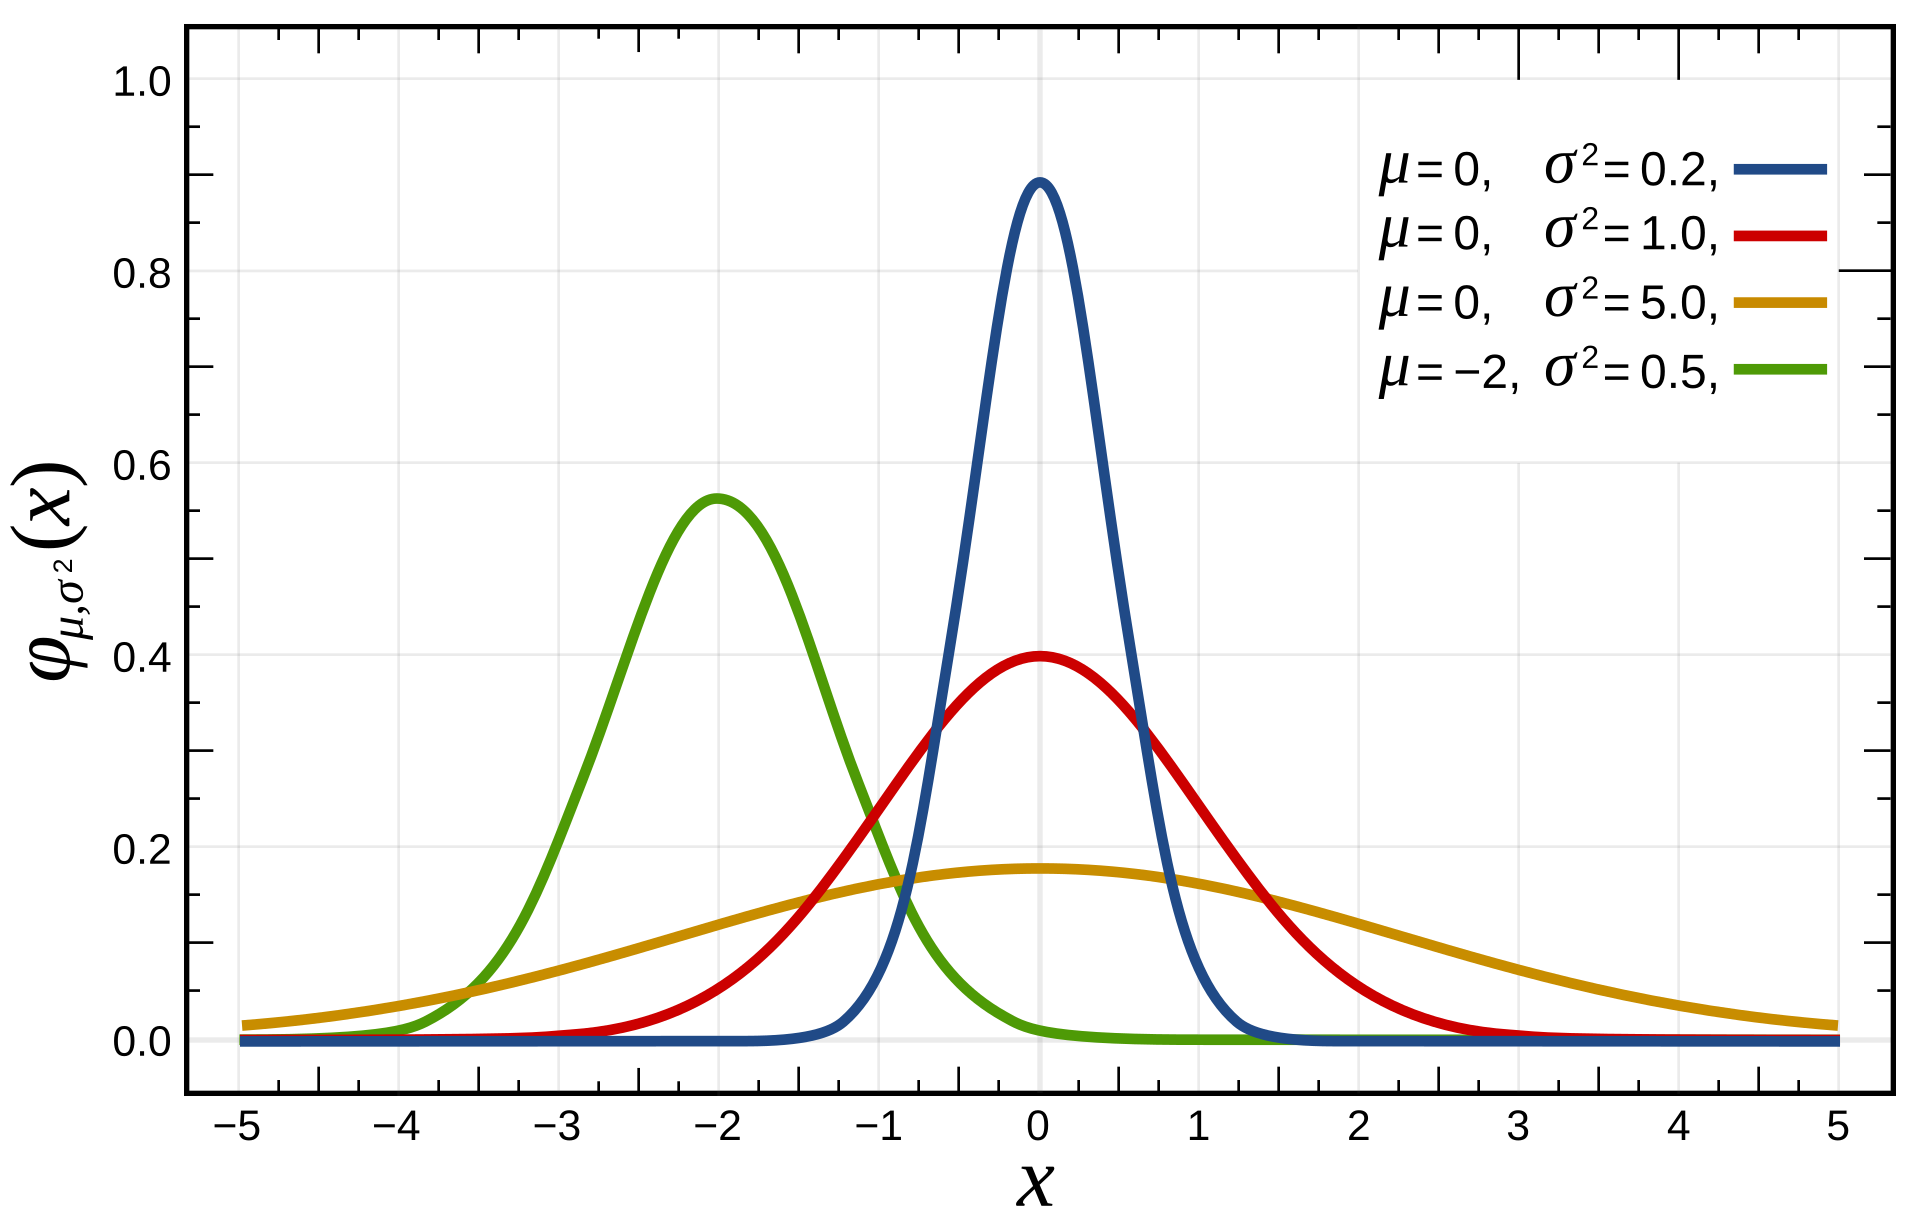
\includegraphics[width=0.45\linewidth]{pics/1d_density.png}
    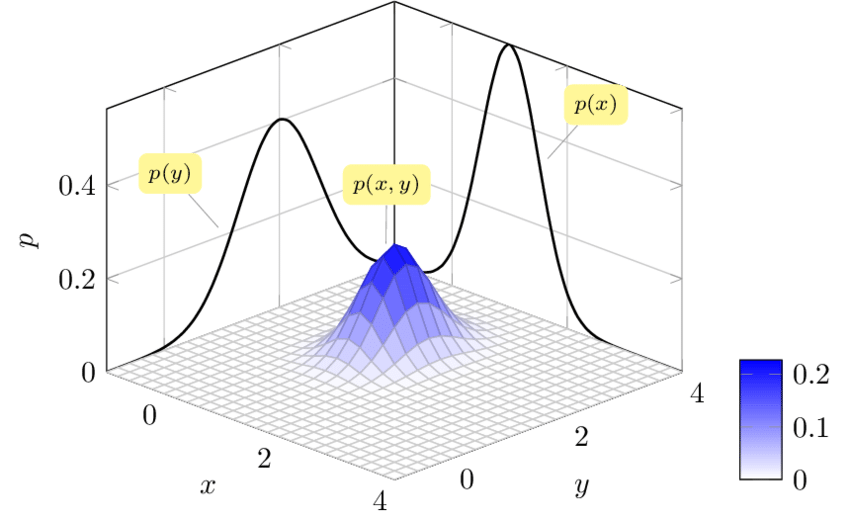
\includegraphics[width=0.45\linewidth]{pics/2d_density.png}
    \caption{Visualization of 1d and 2d Gaussian densities}
    \label{fig:densities_visualization}
\end{figure}

Clearly, the following properties hold
\begin{align}
    \forall x \in \Omega\,,\; p(x) \geq 0\,\; \text{ and }\; \int_\Omega dx\; p(x) = P(\Omega) = 1\,.
\end{align}
Note that this follows from the definition of the random variable.
However, quite often people see some non-negative function $f(x) \geq 0$, and they prove that $\int_\Omega dx\; f(x) < \infty$, i.e. the function is normalizable. 
Then they jump to defining the corresponding probability density function as
\begin{align}
    p(x) = \frac{f(x)}{\int_\Omega dx\; f(x)}\,,
\end{align}
because if the function $f(x)$ is good enough it is true, and because it is useful in practice \kir{which is the whole point of the Monte Carlo methods}.

\begin{example}
    Consider $f(x) = \exp\left(-\frac{1}{2}x^2\right)$, find the corresponding density by finding the normalization constant $\int_{\mathbb{R}} dx\; f(x)$.
\end{example}
\begin{proof}
Let's denote
\begin{align}
    Z \coloneqq \int_{\mathbb{R}} dx\;\exp\left(-\frac{1}{2}x^2\right)\,,
\end{align}
then we have
\begin{align}
     Z^2 = \int_{\mathbb{R}^2} dxdy\;\exp\left(-\frac{1}{2}(x^2+y^2)\right)\,.
\end{align}
Taking $x = r\cos \phi\,, y = r\sin \phi$, we have
\begin{align}
    Z^2 = \int_0^{2\pi}d\phi\;\int_0^\infty dr\;\exp\left(-\frac{1}{2}r^2\right)r = 2\pi \int_0^\infty dy\;\exp\left(-y\right) = 2\pi\,.
\end{align}
Thus, we have
\begin{align}
    p(x) = \frac{1}{\sqrt{2\pi}}\exp\left(-\frac{1}{2}x^2\right)\,.
\end{align}
\end{proof}

\begin{mybox}
\begin{definition}[Normal distribution]\label{def:normal_pdf}
    The density of the Normal distribution or Gaussian distribution is given by the following formula
    \begin{align}
        \Normal(x\cond \mu, \sigma^2) = \frac{1}{\sqrt{2\pi\sigma^2}}\exp\left(-\frac{1}{2\sigma^2}(x-\mu)^2\right)\,.
    \end{align}
    For $\mu=0,\sigma=1$, we call it the \textit{standard} normal distribution.
\end{definition}
\end{mybox}

\subsection{Joint, Marginal, Conditional distributions}

Consider two random variables $X,Y$ that we observe together.
The joint distribution of these random variables is another random variable, which space of outcomes and the corresponding sigma-algebra can be formally constructed using \cref{def:rv}.

\begin{mybox}
\begin{definition}[Joint distribution]\label{def:joint_dist}
    Consider two random variables $X$ with $(\Omega_x, \mathcal{F}_x, P_x)$ and $Y$ with $(\Omega_y, \mathcal{F}_y, P_y)$, then we can define
    \begin{enumerate}
        \item $\Omega = \Omega_x \times \Omega_y$, i.e. the joint outcome space is the direct product of the outcome spaces.
        \item $\mathcal{F} = \mathcal{F}_x \times \mathcal{F}_y$, the product of sigma-algebras can be constructed as the minimal sigma-algebra that contains the set $\{(A_1, A_2): A_1 \in \mathcal{F}_x\,,\; A_2 \in \mathcal{F}_y\}$.
        \item $P: \mathcal{F} \to [0,1]$, and, importantly, it cannot be defined simply through the knowledge of $X$ and $Y$. We have to define this probability measure from other principles, e.g. the observations that we collected by observing $X$ and $Y$ simultaneously.
    \end{enumerate}
\end{definition}
\end{mybox}
Once again, this definition is something that tells us that we have the right to reason about these things, but doesn't give us the tools to reason.

In practice, we usually start from the joint probability or the joint density because it contains the full information about all the random variables involved.
That is, for the discrete variables $\{X_i\}_{i=1}^n$ taking values $x_i$ in integer numbers $\mathbb{Z}$, the joint probability is usually defined as a function that maps integers to probability values, i.e.
\begin{align}
    P: \mathbb{Z}^n \to [0,1]\,, \text{ and for the value at given point we write } P(X_1 = x_1, \ldots, X_n = x_n) = P(x_1, \ldots, x_n)\,.
\end{align}
For the continuous random variables, we define the joint distribution through the joint density. 
That is, for the random variables $\{X_i\}_{i=1}^n$ taking values $x_i$ in the Euclidean space $\mathbb{R}^m$ (not necessarily of the same dimension), we have the density function $p$ that evaluates probabilities
\begin{align}
    \int_A dx\; p(x) = P(X \in A)\,,
\end{align}
where $A$ is in the joint sigma-algebra, $X$ is the joint outcome and $P$ is defined as the probability measure on the joint sigma-algebra.
Clearly, the following holds for the density function
\begin{align}
    p(x_1,\ldots, x_n) \geq 0\,, \;\; \int_{\mathbb{R}^{mn}} dx_1\ldots dx_n\; p(x_1,\ldots,x_n) = 1\,.
\end{align}
Note that there is not much difference between what we considered for the single random variable.
All the differences are hidden in the way we construct the Kolmogorov triplet.

Interesting differences appear when we start ``disassembling'' the joint distribution back into individual random variables and study relations between these variables.
Consider the following function
\begin{align}
    F(x) \coloneqq \sum_{y \in \mathbb{Z}} P(X = x, Y = y)\,,
\end{align}
where $P(X = x, Y = y)$ is the probability function of random variables $X$ and $Y$ and we sum over all possible values of $Y$.
Note that we are summing over disjoint outcomes \kir{indeed, we can't observe $Y$ to take two different values and our outcome space is the product of outcome spaces of $X,Y$}.
We can rewrite it as follows
\begin{align}
    F(x) \coloneqq \sum_{y \in \mathbb{Z}} P(X = x, Y = y) = P(\cup_{y \in \mathbb{Z}} (X = x, Y = y)) = P((X = x, Y \in \Omega_y)) = P(X = x)\,,
\end{align}
where in the last transition we drop the dependency on $Y$ since it always holds.
This motivates the following definition.

\begin{mybox}
\begin{definition}[Marginal distribution]\label{def:marg_dist}
    For the discrete random variables $X,Y$, the marginal distributions of $X$ and $Y$ are defined as follows
    \begin{align}
        P(x) \coloneqq \sum_y P(x,y)\,, \; P(y) \coloneqq \sum_x P(x,y)\,.
    \end{align}
    For the continuous random variables $X,Y$, the probability density function of the marginal distribution of $X$ is defined as follows
    \begin{align}
        p(x) \coloneqq \int_{\Omega_y} dy\; p(x,y)\,,\; p(y) \coloneqq \int_{\Omega_x} dx\; p(x,y)\,.
    \end{align}
\end{definition}
\end{mybox}

You can think about marginalization as of projection of the joint distribution to one of the ``planes'' corresponding to some random variable. \kir{Nobody stops you from defining a new plane in the joint space and projecting to it}
In the space of observations it corresponds to ``forgetting'' or ``erasing'' the information about $Y$, e.g. if you particles hitting a detector, you can register only one of the coordinates, which corresponds to the marginalization of the joint distribution of coordinates.

In practice, one of the most important concepts is the conditioning.
Intuitively, it corresponds to querying your database with something like "select all the musicians that are 27 years old".
More formally, you can consider all the events $\{(X = i, Y=y)\}_{i \in \mathbb{Z}}$, i.e. we fix the value of $Y$ at $y$ and make a collection of all such events by varying $X$.
Note that clearly $P(X = i, Y = y) \geq 0$ for all $i$, hence it is almost a valid probability function, the only problem is that it doesn't normalize to $1$, i.e.
\begin{align}
    \sum_{i\in \mathbb{Z}} P(X = i, Y = y) < 1\,,
\end{align}
because $y$ is fixed and we can't sum over all events in the joint outcome space $\Omega$.
This function, though, makes total sense, and we can think about events of the type ``$X < 0$ and $Y = 6$''.
The solution to this problem is to define a new random variable that corresponds to the ``slice'' of the entire outcome space where $Y = y$.
This leads to the following \textit{definition}!

\begin{mybox}
\begin{definition}[Conditional distribution]\label{def:cond_dist}
    For the discrete random variables $X,Y$, the conditional distribution of $X$ for $Y = y$ is defined as
    \begin{align}
        P(X = x\cond Y = y) \coloneqq \frac{P(X = x, Y = y)}{P(Y = y)}\,.
    \end{align}
    For the continuous random variables $X,Y$, the probability density function of the conditional distribution of $X$ for $Y = y$ is defined as
    \begin{align}
        p(x\cond y) \coloneqq \frac{p(x,y)}{p(y)}\,.
    \end{align}
\end{definition}
\end{mybox}
The vertical line in the notation separates the random variables from the conditions.
In other words, $p(x\cond y)$ defines a random variable on $X$ but not on $y$, this is easy to see by evaluating the normalization constants of the conditional distribution.

\begin{corollary}[Normalization of conditional distribution]
    Conditional distribution normalizes to $1$, i.e. defines a valid random variable.
\end{corollary}
\begin{proof}
    By the straightforward accounting exercises, we have
    \begin{align}
        \sum_x P(x\cond y) = \sum_x \frac{P(x,y)}{P(y)} = \frac{1}{P(y)}\sum_x P(x,y) = \frac{1}{P(y)}P(y) = 1\,,
    \end{align}
    and
    \begin{align}
        \int dx\; p(x\cond y) = \frac{1}{p(y)}\int dx\; p(x,y) = \frac{1}{p(y)}p(y) = 1\,.
    \end{align}
\end{proof}
\kir{note that a lot of results translate seamlessly from the discrete case to the continuous (which i have been abusing above by reasoning in the discrete case and then applying for the continuous). This is not always the case, but we can't keep writing everything for both cases all the time. There is no default choice, or a ``better'' choice, the answer might be disappointing for you, but you have to know both and to know all the bridges between both. Thus, by making progress in one of the worlds you can jump to another and get some insights there.}

Note that for different $y$, according to \cref{def:cond_dist}, we have different distributions $p(x\cond y)$.
However, what if it is not the case?
In other words, consider the special case when
\begin{align}
    p(x\cond y) = p(x)\,,\; \forall y.
\end{align}
Then it makes sense to call random variables $X$ and $Y$ independent, because the distribution of $X$ is not anyhow affected by our choice of $y$.
Using \cref{def:cond_dist}, we have
\begin{align}
    \frac{p(x,y)}{p(y)} = p(x)\,, \implies p(x,y) = p(x)p(y)\,.
\end{align}

\begin{mybox}
\begin{definition}[Independent random variables]\label{def:independent_rvs}
    Two random variables $X,Y$ are called independent if their joint pdf is a product of the marginal pdfs, i.e.
    \begin{align}
        p(x,y) = p(x)p(y)\,.
    \end{align}
\end{definition}
\end{mybox}
\kir{Please note that this is not some philosophical definition of independence and you can make some conclusions based on this. 
This is the mathematical definition that means exactly what is written. See example below} 
\begin{example}
    Consider a king on a chess board going forward and backward as shown in \cref{fig:chess_king}. After a big number of steps, the distribution of $X$ and $Y$ coordinates of its position is going to be uniform. However, it doesn't mean that we can't predict where the king will move next.
\end{example}
\begin{figure}[t]
    \centering
    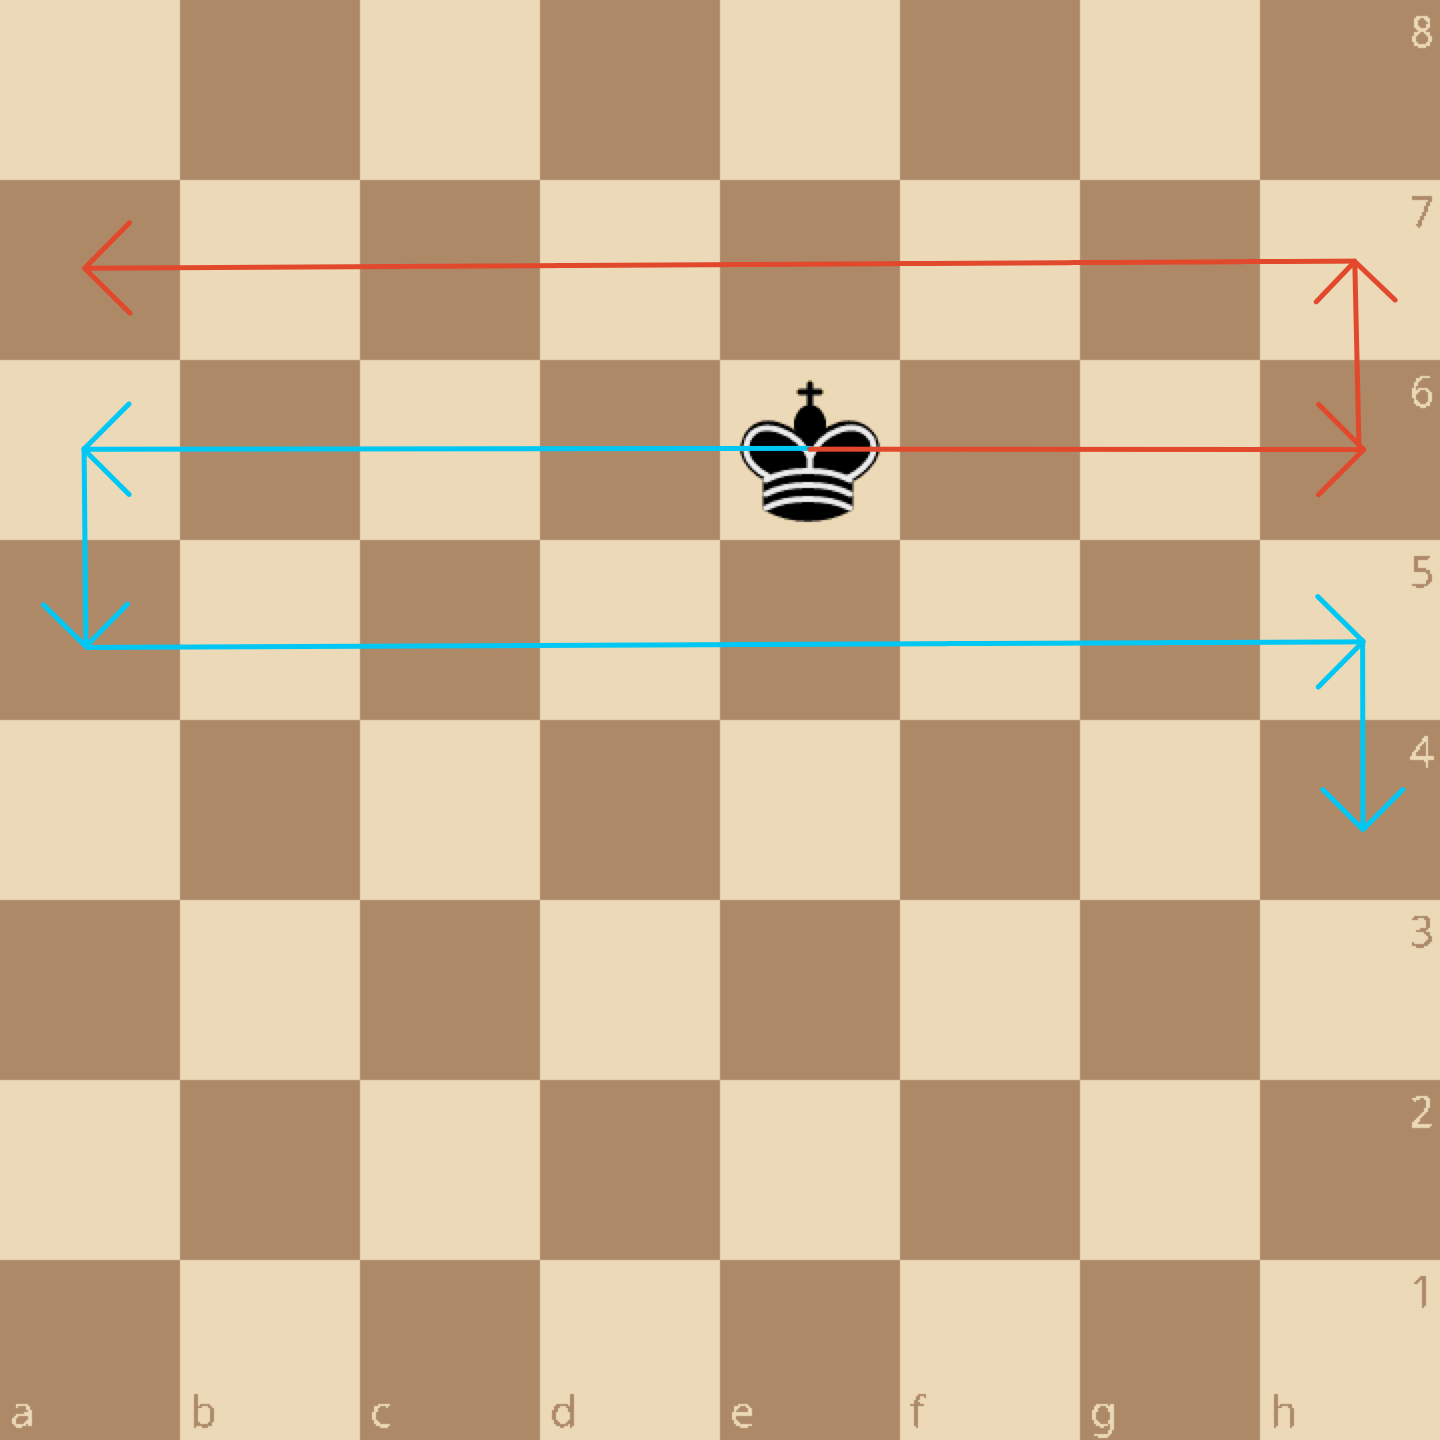
\includegraphics[width=0.3\linewidth]{pics/chess_king.png}
    \caption{Example of the process that generates independent distributions (horizontal and vertical coordinates of the king) but is completely deterministic and predictable}
    \label{fig:chess_king}
\end{figure}

In theory, everything looks symmetric and there is no conceptual difference between $p(x\cond y)$ and $p(y\cond x)$.
However, in practice, we usually know only one of these conditional probabilities and we would like to find the other.

Let's say we know the distribution of $X$ through density $p(x)$ and we know how $Y$ depends on $X$, i.e. we know $p(y\cond x)$.
Oftentimes we are interested in ``inverting the function'' $p(y\cond x)$, i.e. in finding $p(x\cond y)$ \kir{sometimes finding the posterior distribution is called the inverse problem}.
This can be done as follows
\begin{align}
    p(x\cond y) = \frac{p(x,y)}{p(y)} = \frac{p(x,y)}{\int_{\Omega_x} dx\; p(x,y)} = \frac{p(y \cond x)p(x)}{\int_{\Omega_x} dx\; p(y \cond x)p(x)}\,,
\end{align}
where we used the definitions of marginal and conditional distributions.
People refer to this result as Bayes' theorem, as follows.
\begin{theorem}[Bayes' theorem]
\label{th:bayes}
    Conditional density $p(x\cond y)$ can be written using the conditional density $p(y\cond x)$ and the marginal density $p(x)$ as follows
    \begin{align}
        p(x\cond y) = \frac{p(y\cond x)p(x)}{\int_{\Omega_x} dx\; p(y\cond x)p(x)}\,.
    \end{align}
\end{theorem}
This course is devoted to different practical solutions of probabilistic inverse problems based on this result.

\begin{exercise}[Medical Tests]
    Consider the test $t$ for some disease $d$, which conditional distribution $p(t\cond d)$ is defined in the table below. Assuming that we know the marginal distribution of $d$ ($p(d=1) = 0.5$) for the disease, find $p(d = 1\cond t = 1)$
    \begin{center}
    \begin{tabular}{c|cc}
         & $p(t = 1\cond d)$ & $p(t = 1\cond d)$  \\
        \midrule
        d=1 & 0.99 & 0.01 \\
        d=0 & 0.01 & 0.99
    \end{tabular}
    \end{center}
    How the result changes if the disease is very rare ($p(d=1) = 10^{-4}$)?
\end{exercise}

\begin{example}
    Consider the discrete distribution $P(Y = 0) = P(Y = 1) = 1/2$ and the continuous distribution $X\cond Y$ which has the density $\Normal(x\cond y, \sigma^2)$.
    Using the Bayes' theorem, we have
    \begin{align}
        P(Y = 1 \cond x) =~& \frac{p(x\cond y= 1)P(Y=1)}{p(x\cond y= 0)P(Y=0) + p(x\cond y= 1)P(Y=1)}\\
        =~& \frac{\Normal(x\cond 1,\sigma^2)}{\Normal(x\cond 0,\sigma^2) + \Normal(x\cond 1,\sigma^2)} = \frac{\exp\left(-\frac{1}{2\sigma^2}(x-1)^2\right)}{\exp\left(-\frac{1}{2\sigma^2}(x-1)^2\right) + \exp\left(-\frac{1}{2\sigma^2}x^2\right)} \\
        =~& \frac{1}{1 + \exp\left(-\frac{1}{2\sigma^2}\left[x^2 - x^2 +2x - 1\right]\right)} = \frac{1}{1 + \exp\left(-\frac{1}{2\sigma^2}\left[2x - 1\right]\right)}
    \end{align}
    The resulting probability depends on $x$ and is described by the sigmoid function (see \cref{fig:sigmoids})
\end{example}

\begin{figure}[t]
    \centering
    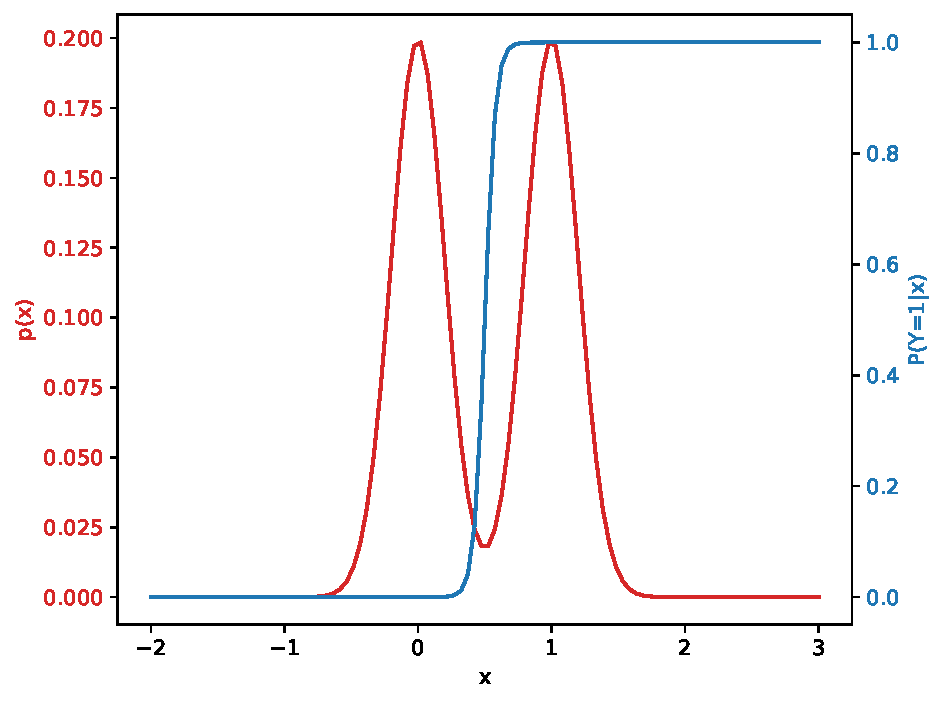
\includegraphics[width=0.45\linewidth]{pics/sigmoid_sharp.pdf}
    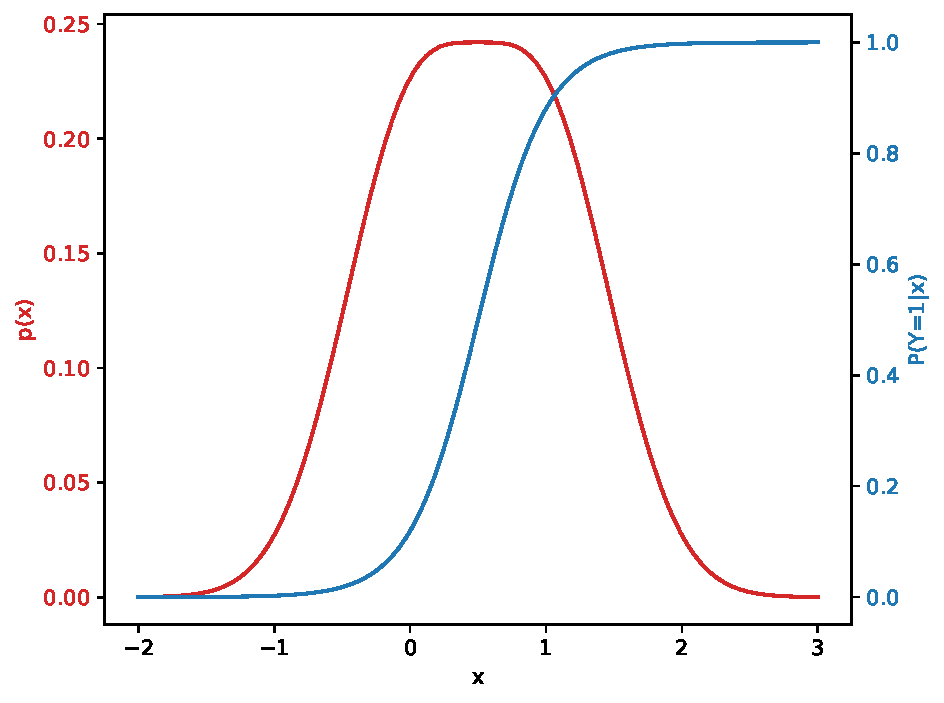
\includegraphics[width=0.45\linewidth]{pics/sigmoid_mix.pdf}
    \caption{Density $p(x)$ and the probability $P(Y=1\cond x)$ for $\sigma=0.2$ (left) and $\sigma=0.5$ (right).}
    \label{fig:sigmoids}
\end{figure}

\begin{mybox}
\begin{definition}[Bernoulli random variable]\label{def:bern_rv}
    The random variable $X$ defined on two states $\Omega = \{0,1\}$ \kir{the states can be anything, ofc} defines the Bernoulli random variable, i.e.
    \begin{align}
        X = \begin{cases}
            1\,, \; \text{ with prob. } \; \theta\,,\\
            0\,, \; \text{ with prob. } \; (1-\theta)\,,
        \end{cases}
        \label{eq:bernoulli_def}
    \end{align}
    where $\theta \in [0,1]$ is a parameter. For $\theta=1/2$, some people call this random variable "fair coin".
\end{definition}
\end{mybox}

Oftentimes, we have a number of \textit{independent} Bernoulli random variables and we want to reason about how many of them equal $1$ and how many of them equal $0$.
First, we will rewrite the probability function of a single Bernoulli variable as follows
\begin{align}
    P(x\cond \theta) = \theta^x (1-\theta)^{1-x}\,,
\end{align}
which, as you can see, corresponds to \cref{eq:bernoulli_def}.
However, now we can multiply this probability functions according to \cref{def:independent_rvs}, i.e.
\begin{align}
    P(x_1,\ldots,x_n\cond \theta) = \theta^{\sum_i x_i} (1-\theta)^{\sum_i (1-x_i)}\,,
\end{align}
which serves as a motivation to another random variable in the following definition.

\begin{mybox}
\begin{definition}[Binomial random variable]\label{def:binomial_rv}
    Consider $n$ \textit{independent} Bernoulli random variables with the parameter $\theta$. The Binomial random variable $X$ is defined as the \textbf{number} of Bernoulli variables that are equal $1$, i.e.
    \begin{align}
        P(X = k \cond \theta, n) = C_n^k \theta^k (1-\theta)^{n-k}\,.
    \end{align}
\end{definition}
\end{mybox}

\begin{exercise}
    Prove the formula from \cref{def:binomial_rv}.
\end{exercise}

\begin{mybox}
\begin{definition}[Poisson random variable]\label{def:poisson_rv}
    Poisson random variable $X$ with the rate $\lambda$ is defined as
    \begin{align}
        P(X = k\cond \lambda) = \exp(-\lambda)\frac{\lambda^k}{k!}.
    \end{align}
    \kir{usually the Poisson random variable defines some sequence of events happening randomly in time (e.g., earthquakes) that's why it makes sense to call its parameter the ``rate''.}
\end{definition}
\end{mybox}
\begin{exercise}
    Prove additivity of the Poisson random variables, i.e. for $X_1 \sim \text{Poiss}(\lambda_1)$ and $X_2 \sim \text{Poiss}(\lambda_2)$, prove that $X_1 + X_2 \sim \text{Poiss}(\lambda_1+\lambda_2)$.
\end{exercise}

\subsection{Probabilistic Graphical model}

We can always reason about all the present random variables by writing the joint distribution of all of them.
However, oftentimes, there is a lot of structure in the dependencies (according to \cref{def:independent_rvs}) between the variables.
It is very convenient to depict the relations between the variables graphically, that's why the community has agreed on the following definition.

\begin{mybox}
\begin{definition}[Probabilistic Graphical model]\label{def:graph_model}
    \textit{Acyclic directed graph} is defines a probabilistic graphical model in the following way
    \begin{align}
        p(x_1,\ldots,x_n) = \prod_{i=1}^n p(x_i \cond \texttt{parents of } x_i)\,.
    \end{align}
\end{definition}
\end{mybox}
For instance, the graph in \cref{fig:graphical_model} defines the following joint distribution
\begin{align}
    p(H,P,E,D,T) = p(T\cond E) p (E\cond P,D) p(H \cond P)p(P)p(D).
\end{align}

\begin{exercise}
    Draw the probabilistic graphical model for the Markov chain probabilistic model
    \begin{align}
        p(x_1,\ldots,x_n) = p(x_0)\prod_{i=0}^{n-1}p(x_{i+1}\cond x_i)\,,
    \end{align}
    for the auto-regressive probabilistic model
    \begin{align}
        p(x_1,\ldots,x_n) = p(x_0)\prod_{i=0}^{n-1}p(x_{i+1}\cond x_i,x_{i-1}\ldots, x_0)\,.
    \end{align}
\end{exercise}

\begin{exercise}
\label{exs:graph_model}
    The model consists of the following random variables: the student went to a party $P \in \{0,1\}$, the student has a depression $D \in \{0,1\}$, the student has a headache $H \in \{0,1\}$, results of the exam are good $E \in \{0,1\}$, the teacher is happy $T \in \{0,1\}$. The relations between these variables are given in \cref{fig:graphical_model} and the conditional probabilities are defined as follows
    \begin{center}
    \begin{tabular}{cc|c}
        $P$ & $D$ & $P(E = 0\cond P,D)$  \\
        \midrule
        $1$ & $1$ & $0.999$ \\
        $0$ & $1$ & $0.9$ \\
        $1$ & $0$ & $0.9$ \\
        $0$ & $0$ & $0.01$
    \end{tabular}
    \begin{tabular}{c|c}
        $P$ & $P(H = 1\cond P)$  \\
        \midrule
        $1$ & $0.999$ \\
        $0$ & $0.9$ \\
        & \\
        & \\
    \end{tabular}
    \begin{tabular}{c|c}
        $E$ & $P(T = 1\cond E)$  \\
        \midrule
        $1$ & $0.5$ \\
        $0$ & $0.95$ \\
        & \\
        & \\
    \end{tabular}
    \begin{tabular}{c}
        $P(P = 1) = 0.2$\\
        $P(D = 1) = 0.4$.
    \end{tabular}
    \end{center}
    Find the following probabilities $P(P=1\cond H=1)$, $P(P=1\cond T=0)$, $P(P=1\cond T=0, H=1)$.
\end{exercise}

\begin{figure}[t]
    \centering
    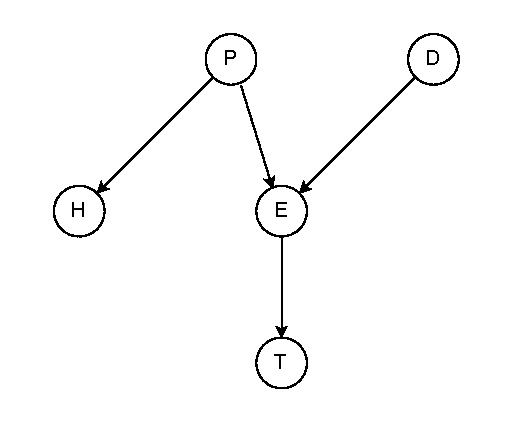
\includegraphics[width=0.4\linewidth]{pics/graphical_model.pdf}
    \caption{Probabilistic graphical model for \cref{exs:graph_model}.}
    \label{fig:graphical_model}
\end{figure}

\subsection{Maximum Likelihood}

In practice, we don't usually know the probabilistic model of some phenomenon, and we would like to design such a model.
The design process of a probabilistic model consists of two main stages:
\begin{enumerate}
    \item Choosing the parametric family of the probabilistic model, i.e. defining how exactly the density value (or probability) $p(x\cond \theta)$ depends on the parameters $\theta$.
    \item Estimating the parameters $\theta$ from the given dataset of observations $\{x_1,\ldots, x_N\}$.
\end{enumerate}

Let's assume that we know exactly the parametric family $p(x\cond \theta)$, i.e. we know for sure that the data we are modeling was generated according to this distribution.
Then one can use the maximum likelihood principle to estimate the parameters $\theta$ from the data.

\begin{mybox}
\begin{definition}[Maximum likelihood]
\label{def:mle}
    For the given parametric family $p(x\cond \theta)$, and the empirical data $\{x_1,\ldots, x_N\}$, Maximum Likelihood Estimator (MLE) of parameters $\theta \in \Theta$ is defined as
    \begin{align}
        \theta_{\text{MLE}} = \argmax_{\theta \in \Theta} p(\{x_1,\ldots, x_N\}\cond \theta)\,,
    \end{align}
    where the density (or probability) $p(\{x_1,\ldots, x_N\}\cond \theta)$ is called likelihood.
\end{definition}
\end{mybox}
If the data was acquired through repeating the same experiment over and over again with the same conditions, it is reasonable to assume \kir{this is a very big and crucial assumption for statistics and machine learning} that the observations $\{x_1,\ldots, x_N\}$ are iid, i.e.
\begin{align}
    p(\{x_1,\ldots, x_N\}\cond \theta) = \prod_{i=1}^N p(x_i\cond \theta)\,.
\end{align}
Under this assumption it's convenient to introduce the following definition.
\begin{mybox}
\begin{definition}[Log-likelihood]\label{def:ll}
    For the given parametric family $p(x\cond \theta)$, and the iid samples $\{x_1,\ldots, x_N\}$, log-likelihood is defined as
    \begin{align}
        \ell(\theta) = \log p(\{x_1,\ldots, x_N\}\cond \theta) = \log \prod_{i=1}^N p(x_i\cond \theta) = \sum_{i=1}^N\log p(x_i\cond \theta)\,.
    \end{align}    
\end{definition}    
\end{mybox}

The maximum likelihood estimator yields closed-form solution for many parametric distribution just by writing down the necessary conditions for the maximum.
\begin{example}[MLE for the Binomial distribution]
    Consider $\mathcal{D}= \{x_1,\ldots,x_N\}$ --- iid samples from the Binomial distribution $\text{Binom}(x\cond n, \theta)$. 
    The log-likelihood for $\theta$ is
    \begin{align}
        \ell(\theta) = \sum_{i=1}^N \log \left(C_{n}^{x_i}\theta^{x_i}(1-\theta)^{n-x_i}\right) = \sum_{i=1}^N  \left(\log C_{n}^{x_i} + x_i\log \theta + (n-x_i)\log(1-\theta)\right)\,.
    \end{align}
    From the maximum likelihood principle, we have
    \begin{align}
        0 =~& \deriv{}{\theta}\ell(\theta) = \sum_{i=1}^N  \left(x_i\frac{1}{\theta} + (n-x_i)\frac{1}{1-\theta}\right)\,,\\
        (1-\theta)\sum_i x_i =~& \theta\sum_i(n-x_i)\\
        \theta_{\text{MLE}} =~& \frac{\sum_i x_i}{\sum_i n} = \frac{1}{N}\sum_i \frac{x_i}{n}\,.
    \end{align}
    It is the average success rate over all the experiments.
\end{example}

The following theorem is one of the main motivations for using MLE.
\begin{theorem}[Convergence of MLE]
    Consider the set of iid samples $\mathcal{D} = \{x_1,\ldots, x_N\}$ from the categorical distribution $P(x\cond \theta^*)$
    \begin{align}
        P(x = k \cond \theta^*) = \theta^*_k\,,\; \theta^*_k \geq 0\;\forall k\,.
    \end{align}
    The maximum likelihood estimator of $\theta$ (under the ground true probabilistic model) converges (in the number of samples) to the ground true parameters, i.e.
    \begin{align}
        \lim_{N\to\infty} \theta_{\text{MLE}} = \theta^*\,.
    \end{align}
\end{theorem}
\begin{proof}
    The log-likelihood of the dataset is
    \begin{align}
        \ell(\theta) =~& \frac{1}{N}\sum_{i=1}^N\log P(x_i\cond \theta) = \frac{1}{N}\sum_{k=1}^MN_k\log P(x_i=k\cond \theta)\\
        =~& \frac{1}{N}\sum_{k=1}^MN_k\log \theta_k = \sum_{k=1}^M\frac{N_k}{N}\log \theta_k\,,
    \end{align}
    where $N_k$ is the number of samples that equal $k$, i.e. $N_k = |\{x \in \mathcal{D}  \cond x = k\}|$.
    From the maximum likelihood principle, we have
    \begin{align}
        \theta_{\text{MLE}} = \argmax \ell(\theta)\,, \;\text{ s.t. }\; \sum_{k=1}^M\theta_k = 1\,,\; \theta_k \geq 0\;\forall k\,.
    \end{align}
    The corresponding Largangian is
    \begin{align}
        \mathcal{L}(\theta) = \ell(\theta) + \lambda \sum_{k=1}^M(\theta_k - 1)\,,
    \end{align}
    and the necessary condition for the optimum is
    \begin{align}
        \forall k\,,\;0 = \deriv{\ell(\theta)}{\theta_k}  + \lambda = \frac{1}{\theta_k}\frac{N_k}{N}  + \lambda \implies \theta_k = \frac{N_k}{N}\,.
    \end{align}
    Thus, we have
    \begin{align}
        \theta_{\text{MLE}} = \begin{bmatrix}
            \ldots\\
            \frac{N_k}{N}\\
            \ldots
        \end{bmatrix}\,.
    \end{align}
    For the limit of the infinite number of samples, we have
    \begin{align}
        \lim_{N\to\infty} (\theta_{\text{MLE}})_k = \lim_{N\to\infty}\frac{N_k}{N} = P(X=k\cond \theta^*) = \theta^*_k\,.
    \end{align}
\end{proof}
Thus, we have demonstrated that if we know the probabilistic model $p(x\cond\theta)$ exactly, then for any given precision of the parameter estimation $\theta$ we can collect the dataset $\mathcal{D}$ large enough to satisfy this precision.

\begin{exercise}
    Consider $x_1,\ldots,x_N$ --- iid samples from the Normal distribution $\mathcal{N}(x\cond \mu, \sigma)$. Find the maximum likelihood estimation of $\mu,\sigma$.
\end{exercise}

\begin{exercise}
    Consider $x_1,\ldots,x_N$ --- iid samples from the Poisson distribution $\text{Poiss}(\lambda)$. Find the maximum likelihood estimation of $\lambda$.
\end{exercise}

\begin{proposition}[MLE for regression]
    Consider the dataset $\mathcal{D} = \{(x_i, y_i)\}_{i=1}^N$, where $x \in \mathbb{R}^d$ and $y \in \mathbb{R}$.
    Assuming the following probabilistic model for the dataset
    \begin{align}
        y = f(x;\theta) + \eps\,, \eps \sim \Normal(\eps\cond 0,\sigma^2)\,,
    \end{align}
    where $f$ is some known function.
    find the maximum likelihood estimation of $\theta$ and $\sigma$
\end{proposition}
\begin{proof}
    First, let's rewrite the probabilistic model in a more familiar form
    \begin{align}
        p(y\cond x,\theta,\sigma) = \Normal(y\cond f(x;\theta), \sigma^2)\,.
    \end{align}
    Note that here $y$ is conditioned on the features $x$, parameters of the mean predictor $\theta$ and the standard deviation $\sigma$.
    The log-likelihood of this probabilistic model is
    \begin{align}
        \ell(\theta,\sigma) = \frac{1}{N}\sum_{i=1}^N \log \Normal(y_i\cond f(x_i;\theta), \sigma^2) = \frac{1}{N}\sum_{i=1}^N \left[-\frac{1}{2\sigma^2}(y_i-f(x_i;\theta))^2 - \frac{1}{2}\log (2\pi\sigma^2)\right]\,.
    \end{align}
    Hence, we have
    \begin{align}
        \theta_{\text{MLE}} =~& \argmax_\theta \ell(\theta,\sigma) = \argmax_\theta \ell(\theta,\sigma) \frac{1}{N}\sum_{i=1}^N \left[-\frac{1}{2\sigma^2}(y_i-f(x_i;\theta))^2 - \frac{1}{2}\log (2\pi\sigma^2)\right]\\
        =~& \argmin_\theta \frac{1}{N}\sum_{i=1}^N \left[\frac{1}{2\sigma^2}(y_i-f(x_i;\theta))^2\right] = \argmin_\theta \frac{1}{N}\sum_{i=1}^N (y_i-f(x_i;\theta))^2\,.
    \end{align}
    Thus, MLE is equivalent to Mean-Squared Error (MSE) loss function.
    For $\sigma_{\text{MLE}}$, we have
    \begin{align}
        0 = \deriv{\ell(\sigma)}{\sigma} =~& \frac{1}{N}\sum_{i=1}^N \left[\frac{1}{\sigma^3}(y_i-f(x_i;\theta))^2 - \frac{1}{\sigma}\right] = \frac{1}{N}\sum_{i=1}^N \frac{1}{\sigma^3}(y_i-f(x_i;\theta))^2 - \frac{1}{\sigma}\,,\\
        \sigma_{\text{MLE}}^2 = ~& \frac{1}{N}\sum_{i=1}^N (y_i-f(x_i;\theta_\text{MLE}))^2\,.
    \end{align}
    Thus, the MLE for $\sigma$ equals the average error that persists for $\theta_{\text{MLE}}$.
\end{proof}

\begin{exercise}
    MLE for Laplace residuals
\end{exercise}

\begin{exercise}
    MLE for logistic regression
\end{exercise}


\clearpage
\section{Basics of Bayesian statistics}

\begin{figure}[h]
    \centering
    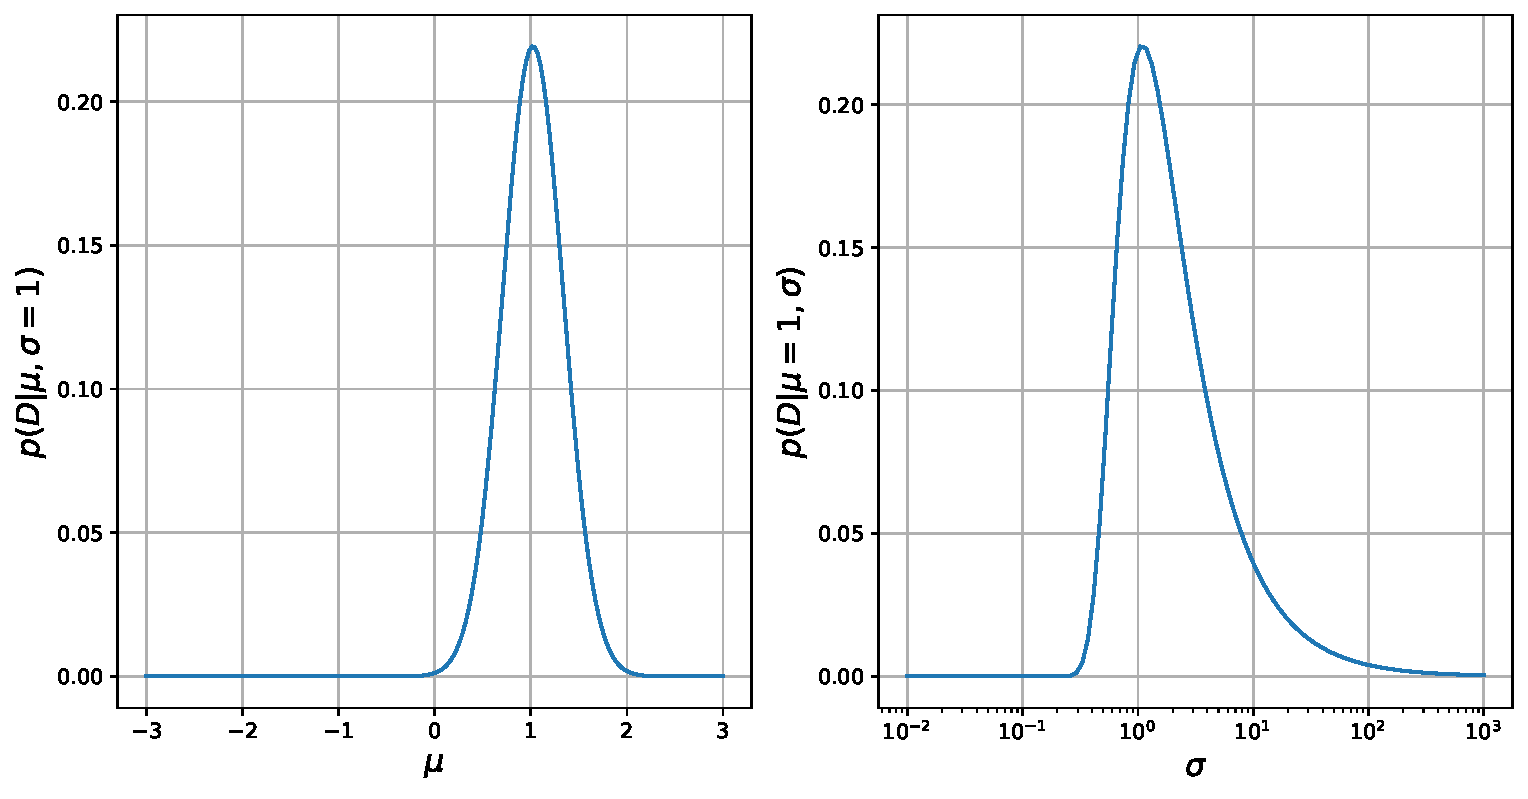
\includegraphics[width=0.9\linewidth]{pics/likelihood.pdf}
    \caption{Likelihood of the dataset $\mathcal{D}$ of $10$ samples from $\Normal(x\cond \mu = 1, \sigma^2 = 0.5^2)$.}
    \label{fig:likelihood}
\end{figure}

Maximum likelihood gives us a point-estimate of the parameters of our probabilistic model, and if the model is correct \kir{no} then we know that with the number of data points our estimate converges to the ground true value.
However, what if we plot the likelihood for other values of parameters?
In \cref{fig:likelihood}, we see that the likelihood function depending on the parameter also looks like some density, i.e. it is a positive function that vanishes at the infinity so it might be normalizable.

Indeed, consider the likelihood of some dataset $\mathcal{D}$, that corresponds to the normal model $p(x\cond \theta) = \Normal(x\cond \mu, \sigma^2)$. 
For the likelihood w.r.t $\mu$ (and some fixed $\sigma$) it's very straightforward
\begin{align}
    p(\mathcal{D}\cond \mu, \sigma=1) =~& \frac{1}{\sqrt{2\pi}}\exp\left(-\frac{1}{2}\sum_{i=1}^N(x_i-\mu)^2\right) = \frac{1}{\sqrt{2\pi}}\exp\left(-\frac{1}{2}\left(\sum_ix_i^2-2\mu\sum_i x_i + N\mu^2\right)\right)\\
    =~&\frac{1}{\sqrt{2\pi}}\exp\left(-\frac{\sqrt{N}^2}{2}\left(\mu^2-2\mu\hat{\mu} + \hat{\mu}^2 - \hat{\mu}^2 + \frac{1}{N}\sum_i x_i^2\right) \right)\\
    =~&\frac{1}{\sqrt{2\pi}}\exp\left(-\frac{1}{2(1/\sqrt{N})^2}\left(\mu-\hat{\mu}\right)^2 - \hat{\mu}^2 + \frac{1}{N}\sum_i x_i^2\right)\propto\Normal\left(\mu\cond \hat{\mu},\frac{1}{N}\right)\,,
    \label{eq:normal_likelihood}
\end{align}
where $\hat{\mu} = \frac{1}{N}\sum_i x_i$.
Thus, we see that the likelihood is proportional to the normal distribution w.r.t. $\mu$. 
However, it is the normal distribution w.r.t $\mu$ because it doesn't normalize to $1$. \kir{in some cases the function can be not normalizable in principle}

For the likelihood w.r.t. $\sigma$ (and fixed $\mu$), we have
\begin{align}
    p(\mathcal{D}\cond \mu=0, \sigma) =~& \frac{1}{\sqrt{2\pi\sigma^2}}\exp\left(-\frac{1}{2\sigma^2}\sum_{i=1}^Nx_i^2\right) \propto \left(\frac{1}{\sigma^2}\right)^{N/2}\exp\left(-\left(\frac{1}{2}\sum_{i=1}^Nx_i^2\right)\frac{1}{\sigma^2}\right)\\
    =~& \gamma^{N/2}\exp\left(-\left(\frac{1}{2}\sum_{i=1}^Nx_i^2\right)\gamma\right) \propto \mathcal{G}\left(\gamma\cond N/2+1, \frac{1}{2}\sum_{i=1}^Nx_i^2\right)\,,
\end{align}
where we introduced the parameter $\gamma = 1/\sigma^2$.
The likelihood function is proportional to the density of the gamma distribution (see below), but it's not the gamma distribution because it doesn't normalize to $1$.

\begin{definition}[Gamma distribution]\label{def:gamma_pdf}
    Consider the density proportional to 
    \begin{align}
        \mathcal{G}(x\cond a,b) = \frac{b^a}{\Gamma(a)}x^{a-1}\exp(-b x)\,,
    \end{align}
    where $\Gamma(\cdot)$ is the gamma function.
\end{definition}

To sum up, we see that the likelihood already defines something like a distribution on the set of parameters.
Thus, we should consider treating parameters as random variables!

\subsection{Bayesian reasoning}

When treating parameters as random variables, let's start with the likelihood model, i.e. let's assume that the following holds
\begin{align}
    p(\mathcal{D} \cond \theta) = \prod_i p(x_i\cond \theta)\,,
\end{align}
and the model $p(x\cond \theta)$ is given.
Remember that the entire information about $x$ and $\theta$ is in their joint distribution, whose density we can write down as follows (using \cref{def:cond_dist})
\begin{align}
    \underbrace{p(x,\theta)}_{\text{joint}} = \underbrace{p(x\cond \theta)}_{\text{likelihood}}\underbrace{p(\theta)}_{\text{prior}}\,.
\end{align}
Thus, if we know or introduce the prior distribution $p(\theta)$, we know everything about the random variables $x$ and $\theta$.

Namely, using the definition of the conditional distribution (or \cref{th:bayes}), we can write down the following
\begin{align}
\label{eq:posterior_density}
    p(\theta \cond \mathcal{D}) = \frac{p(\mathcal{D} \cond \theta)p(\theta)}{p(\mathcal{D})} = \frac{p(\mathcal{D} \cond \theta)p(\theta)}{\int d\theta\; p(\mathcal{D} \cond \theta)p(\theta)}\,.
\end{align}
\begin{mybox}
\begin{definition}[Posterior Distribution]\label{def:posterior}
    Distribution corresponding to the density $p(\theta \cond \mathcal{D})$ from \cref{eq:posterior_density} is called the posterior distribution.
\end{definition}
\end{mybox}

Let's try choosing prior $p(\theta)$ such that we know the posterior distribution $p(\theta\cond \mathcal{D})$ immediately.

\begin{example}
    For the likelihood, consider the normal distribution with the parameter $\mu$ and fixed $\sigma$
    \begin{align}
        p(x\cond \theta) = \Normal(x\cond \mu,\sigma^2=1)\,.
    \end{align}
    From \cref{eq:normal_likelihood}, we already have
    \begin{align}
        p(\mathcal{D}\cond \mu, \sigma=1)\propto\Normal\left(\mu\cond \hat{\mu},\frac{1}{N}\right) \propto \exp\left(-\frac{1}{2(1/\sqrt{N})^2}(\mu-\hat{\mu})^2\right)\,,
    \end{align}
    where $\hat{\mu} = \frac{1}{N}\sum_i x_i$.
    The posterior distribution is defined as
    \begin{align}
        p(\mu \cond \mathcal{D}) \propto \exp\left(-\frac{1}{2(1/\sqrt{N})^2}(\mu-\hat{\mu})^2\right)p(\mu)\,.
    \end{align}
    Let's choose the prior distribution $p(\mu)$ so that the functional form of the posterior distribution is the same as of the prior distribution.
    That is, consider $p(\mu) = \Normal(\mu\cond m,s^2)$
    \begin{align}
        p(\mu \cond \mathcal{D}) \propto~& \exp\left[-\frac{1}{2(1/\sqrt{N})^2}(\mu-\hat{\mu})^2-\frac{1}{2s^2}(\mu-m)^2\right] \propto \exp\left[-\frac{1}{2}\left(\left(N+\frac{1}{s^2}\right)\mu^2 -2\mu\left(N\hat{\mu}+\frac{m}{s^2}\right)\right)\right] \\
        =~& \exp\left[-\frac{1}{2}\left(\frac{Ns^2+1}{s^2}\right)\left(\mu^2 -2\mu\left(\frac{Ns^2\hat{\mu}+m}{Ns^2+1}\right)\right)\right] \\
        \propto~& \exp\left[-\frac{1}{2}\left(\frac{Ns^2+1}{s^2}\right)\left(\mu -\left(\frac{Ns^2\hat{\mu}+m}{Ns^2+1}\right)\right)^2\right] = \Normal\left(\mu\cond \frac{Ns^2\hat{\mu}+m}{Ns^2+1}, \frac{s^2}{Ns^2+1}\right)
    \end{align}
\end{example}
Note that
\begin{align}
    \lim_{N\to\infty} \frac{Ns^2\hat{\mu}+m}{Ns^2+1} = \lim_{N\to\infty}\hat{\mu} = \lim_{N\to\infty}\mu_{\text{MLE}}\,,
\end{align}
and for large $N$, we have
\begin{align}
    \frac{s^2}{Ns^2+1} \approx \frac{1}{N}\,,
\end{align}
as we had before for the likelihood w.r.t. $\sigma$.

By finding the prior such that the posterior is easy to find we have motivated the following definition.
\begin{mybox}
\begin{definition}[Conjugate distribution]\label{def:conjugate_dist}
    For the likelihood $p(x\cond \theta)$, if the parametric family of the posterior $p(\theta\cond x)$ is the same as the parametric family of the prior $p(\theta)$ these distributions are called conjugate.
    Oftentimes, people just say conjugate prior $p(\theta)$ to the likelihood $p(x\cond \theta)$.
\end{definition}
\end{mybox}

\begin{example}
    For the likelihood, consider the normal distribution with the parameter $\sigma$ and fixed $\mu$
    \begin{align}
        p(x\cond \theta) = \Normal(x\cond \mu=0,\sigma^2)\,.
    \end{align}
    From before, we have
    \begin{align}
    p(\mathcal{D}\cond \mu=0, \sigma) \propto \mathcal{G}\left(\gamma\cond N/2+1, \frac{1}{2}\sum_{i=1}^Nx_i^2\right)\,,
    \end{align}
    The posterior distribution is defined as
    \begin{align}
        p(\gamma \cond \mathcal{D}) \propto \gamma^{N/2}\exp\left(-\left(\frac{1}{2}\sum_{i=1}^Nx_i^2\right)\gamma\right)p(\gamma)\,.
    \end{align}
    Let's choose the prior distribution $p(\gamma)$ so that the functional form of the posterior distribution is the same as of the prior distribution.
    That is, consider $p(\gamma) = \mathcal{G}(\gamma\cond a,b)$
    \begin{align}
        p(\gamma \cond \mathcal{D}) \propto \gamma^{N/2}\exp\left(-\left(\frac{1}{2}\sum_{i=1}^Nx_i^2\right)\gamma\right)\gamma^{a-1}\exp(-b\gamma) \propto \mathcal{G}\left(\gamma\cond N/2+a, b+\frac{1}{2}\sum_{i=1}^Nx_i^2\right)\,.
    \end{align}
\end{example}

\begin{exercise}
    Consider $x_1,\ldots,x_N$ --- iid samples from the exponential density function
    \begin{align}
        p(x\cond \lambda) = \lambda\exp(-\lambda x)\,, \;\; x \geq 0\,, \lambda > 0.
    \end{align}
    Find the conjugate prior $p(\lambda)$ and the corresponding posterior $p(\lambda\cond \mathcal{D})$.
\end{exercise}

\begin{exercise}
    Consider $x_1,\ldots,x_N$ --- iid samples from the Poisson distribution $\text{Poiss}(\lambda)$
    \begin{align}
        P(X = k\cond \lambda) = \exp(-\lambda)\frac{\lambda^k}{k!}.
    \end{align}
    Find the conjugate prior $p(\lambda)$ and the corresponding posterior $p(\lambda\cond \mathcal{D})$.
\end{exercise}

\begin{exercise}
    Consider $x_1,\ldots,x_N$ --- iid samples from the Bernoulli distribution $\text{Bernoulli}(\theta)$
    \begin{align}
        p(x\cond \theta) = \theta^x(1-\theta)^{(1-x)}.
    \end{align}
    Find the conjugate prior $p(\theta)$ and the corresponding posterior $p(\theta\cond \mathcal{D})$. Does it matter if instead we consider one sample from the Binomial with probability of success $\theta$ and number of trials $N$?
\end{exercise}

\kir{I'll just put this here}
\begin{mybox}
\begin{definition}[Beta distribution]\label{def:beta_density}
    Consider the density proportional to 
    \begin{align}
        \mathcal{B}(x\cond a,b) = \frac{\Gamma(a+b)}{\Gamma(a)\Gamma(b)}x^{a-1}(1-x)^{b-1} = \frac{1}{B(a,b)}x^{a-1}(1-x)^{b-1}\,,
    \end{align}
    where $\Gamma(\cdot)$ and $B(\cdot)$ are the gamma and beta functions correspondingly.
\end{definition}
\end{mybox}

When it's hard to find the entire posterior distribution, one can use its mode, which is easier to find.
\begin{mybox}
\begin{definition}[Maximum A posteriori (MAP)]\label{def:map}
    The mode of the posterior distribution is called the Maximum A posteriori (MAP) estimate and is defined as follows
    \begin{align}
        \theta_{\text{MAP}} = \argmax_{\theta \in \Theta} p(\theta \cond \mathcal{D}) = \argmax_{\theta \in \Theta} \frac{p(\mathcal{D} \cond \theta)p(\theta)}{p(\mathcal{D})} = \argmax_{\theta \in \Theta} p(\mathcal{D} \cond \theta)p(\theta)\,.
    \end{align}
\end{definition}
\end{mybox}

Finally, to make new prediction, one can take into account all the possible parameters from the posterior distribution.
Namely, let's say we want to get the distribution of observations $x$ after observing the dataset $\mathcal{D}$, then we can write \kir{absolutely mindless mathematical tautology}
\begin{align}
    p(x\cond \mathcal{D}) = \int d\theta\; p(x,\theta \cond \mathcal{D}) = \int d\theta\; p(x \cond \theta, \mathcal{D}) p(\theta \cond \mathcal{D})\,,
\end{align}
after we assume that all the information about the dataset is in our parameters $\theta$.
In other words, having the parameters $\theta$ is all we need for making the probabilistic model, i.e. $p(x \cond \theta, \mathcal{D}) = p(x \cond \theta)$.
Under this strong assumption, we proceed as
\begin{align}
    p(x\cond \mathcal{D}) = \int d\theta\; p(x \cond \theta) p(\theta \cond \mathcal{D}) = \mean_{p(\theta \cond \mathcal{D})} p(x \cond \theta)\,,
\end{align}
i.e. the probabilistic model of $x$, after observing the dataset $\mathcal{D}$ is defined as an average of probabilities/densities over all possible values of parameters sampled from the posterior distribution.
\begin{mybox}
\begin{definition}[Predictive Distribution]\label{def:predictive_dist}
    Given the likelihood $p(x \cond \theta)$ and the posterior $p(\theta \cond \mathcal{D})$, one defines the predictive distribution as follows
    \begin{align}
        p(x\cond \mathcal{D}) = \int d\theta\; p(x \cond \theta) p(\theta \cond \mathcal{D}) = \mean_{p(\theta \cond \mathcal{D})} p(x \cond \theta)\,.
    \end{align}
\end{definition}
\end{mybox}

\subsection{Exponential family}

There is a large and important family of distributions that allows for the Bayesian inference.
\begin{mybox}
\begin{definition}[Exponential family]\label{def:expo_family}
    The exponential family of random variables is all random variables which density has the following functional form
    \begin{align}
        p(x\cond \theta) = \frac{f(x)}{g(\theta)}\exp\left(\theta^Tu(x)\right)\,.
    \end{align}
\end{definition}
\end{mybox}

First, let's play around with the definition.
For instance, let's see what we can get from the normalization of the density.
\begin{align}
    \int dx\; p(x\cond \theta) =~& \int dx\; \frac{f(x)}{g(\theta)}\exp\left(\theta^Tu(x)\right) = 1\,,\\
    g(\theta) =~& \int dx\; f(x)\exp\left(\theta^Tu(x)\right)\,.
\end{align}
It is reasonable to call $g(\theta)$ a normalization constant of this distribution.
Note that the derivative of the normalization constant has interesting properties
\begin{align}
    \deriv{}{\theta_i}g(\theta) =~& \int dx\; f(x)\deriv{}{\theta_i}\exp\left(\theta^Tu(x)\right) = \int dx\; f(x)\exp\left(\theta^Tu(x)\right)u_i(x) = g(\theta)\int dx\; p(x\cond \theta) u_i(x)\,,\\
    \deriv{}{\theta_i}\log g(\theta) =~& g(\theta)\int dx\; p(x\cond \theta) u_i(x) = \mean_{p(x\cond \theta)}u_i(x)\,.
\end{align}
Thus, we have
\begin{proposition}
\label{prop:grad_norm_constant}
    For the density $p(x\cond \theta)$ from the exponential family, we have
    \begin{align}
        \nabla_\theta\log g(\theta) = \mean_{p(x\cond \theta)}u(x)\,.
    \end{align}
\end{proposition}

\begin{exercise}
For the exponential family $p(x\cond \theta) = \frac{f(x)}{g(\theta)}\exp\left(\theta^Tu(x)\right)$, find the expression for
\begin{align}
    \deriv{^2}{\theta_i\theta_j}\log g(\theta) = ?
\end{align}
\end{exercise}

Let's find the maximum likelihood estimator for this family
\begin{align}
    \log p(\mathcal{D}\cond \theta) =~& \sum_{i=1}^N \left[\log f(x_i) - \log g(\theta) + \theta^Tu(x_i)\right]\,,\\
    \nabla_\theta\log p(\mathcal{D}\cond \theta) =~& \sum_{i=1}^N \left[ - \nabla_\theta\log g(\theta) + u(x_i)\right] = 0\,,\\
    \nabla_\theta\log g(\theta) =~& \frac{1}{N}\sum_{i=1}^Nu(x_i)\,.
\end{align}
Using \cref{prop:grad_norm_constant}, we have that, for $\theta_{\text{MLE}}$, the expectation of statistics $u(x)$ equals empirical expectation of statistics $u(x)$ on the observed data, i.e.
\begin{align}
    \mean_{p(x\cond \theta_{\text{MLE}})}u(x) = \frac{1}{N}\sum_{i=1}^Nu(x_i)\,.
\end{align}
Note we need only values of $u(x_i)$ on our data to completely determine the maximum likelihood estimation of our parameters $\theta$. This motivates the following definition
\begin{mybox}
\begin{definition}[Sufficient statistics]\label{def:suff_stats}
When the density $p(x\cond \theta)$ can be factorized as
\begin{align}
    p(x\cond \theta) = p_1(x)p_2(u(x),\theta)\,,
\end{align}
the function $u(x)$ is called sufficient statistics.
\end{definition}
\end{mybox}

\begin{example}
Consider the normal density
\begin{align}
    \Normal(x\cond \mu, \sigma^2) = \frac{1}{\sqrt{2\pi\sigma^2}}\exp\left(-\frac{1}{2\sigma^2}(x-\mu)^2\right) = \frac{1}{\sqrt{2\pi\sigma^2}}\exp\left(-\frac{x^2}{2\sigma^2} + \frac{x\mu}{\sigma^2} -\frac{\mu^2}{2\sigma^2}\right)\,.
\end{align}
From the definition of exponential family, we can write
\begin{align}
    u(x) = \begin{bmatrix}
        x\\
        x^2
    \end{bmatrix}\,,\;\;
    \theta = \begin{bmatrix}
        \frac{\mu}{\sigma^2}\\
        -\frac{1}{2\sigma^2}
    \end{bmatrix}\,,\;\;
    g(\theta)^{-1} = \frac{1}{\sqrt{2\pi\sigma^2}}\exp\left(-\frac{\mu^2}{2\sigma^2}\right) = \sqrt{\frac{-\theta_2}{\pi}}\exp\left(\frac{\theta_1^2}{4\theta_2}\right)\,.
\end{align}
Thus, we have a different parameterization of the normal distribution. Let's find the expectation from this parametric form.
\begin{align}
    \deriv{}{\theta_1}\log g(\theta) =~& -\frac{\theta_1}{2\theta_2} = \mu\,,\\
    \deriv{}{\theta_2}\log g(\theta) =~& -\frac{1}{2\theta_2}+\frac{\theta_1^2}{4\theta_2^2} = \sigma^2 + \mu^2\,.
\end{align}
Hence, we see that we can find expectations of sufficient statistics without integration \kir{integration is principally much harder than differentiation}
\end{example}
When we write down some density in the form of \cref{def:expo_family}, the parameters $\theta$ are called \textit{natural parameters}.

Let's find the conjugate distributions to the exponential family
\begin{align}
    p(\theta\cond \mathcal{D}) \propto~& \prod_i p(x_i\cond \theta)p(\theta) = \left[\prod_i\frac{f(x_i)}{g(\theta)}\right]\exp\left(\sum_i\theta^Tu(x_i)\right)p(\theta)\\
    =~& \left[\prod_i f(x_i)\right]\exp\left(\sum_i\theta^Tu(x_i)\right)\frac{p(\theta)}{g(\theta)^N}\,.
\end{align}
Based on this form, we can choose the prior
\begin{align}
    p(\theta\cond \eta,\nu) = \frac{1}{h(\eta,\nu)}\frac{1}{g(\theta)^\nu}\exp\left(\theta^T\eta\right)\,.
\end{align}
Then
\begin{align}
    p(\theta\cond \mathcal{D}) \propto~& \frac{1}{g(\theta)^N}\exp\left(\sum_i\theta^Tu(x_i)\right)\frac{1}{h(\eta,\nu)}\frac{1}{g(\theta)^\nu}\exp\left(\theta^T\eta\right) \propto \frac{1}{g(\theta)^{\nu+N}}\exp\left(\theta^T\left(\eta +\sum_iu(x_i)\right)\right)\\
    p(\theta\cond \mathcal{D}) \propto~& p(\theta\cond \eta +\sum_iu(x_i),\nu + N)\,.
\end{align}

\begin{exercise}
    Represent the gamma distribution
    \begin{align}
        \mathcal{G}(x\cond a,b) = \frac{b^a}{\Gamma(a)}x^{a-1}\exp(-b x)\,,
    \end{align}
    as a density from the exponential family, find the expectations of the sufficient statistics.
\end{exercise}

\begin{exercise}
    Represent the beta distribution
    \begin{align}
        \mathcal{B}(x\cond a,b) = \frac{\Gamma(a+b)}{\Gamma(a)\Gamma(b)}x^{a-1}(1-x)^{b-1} = \frac{1}{B(a,b)}x^{a-1}(1-x)^{b-1}\,,
    \end{align}
    as a density from the exponential family, find the expectations of the sufficient statistics.
\end{exercise}

\subsection{Maximum Entropy Principle \citep{jaynes1957information}}

Consider a distribution over a finite set of outcomes $\{1,\ldots,M\}$ with probabilities $\{p_1,\ldots,p_M\}$. 
Clearly, when $p_1 = 1$ and $p_i = 0\,, i = 2,\ldots, M$ the distribution becomes degenerate and we can say for sure that all the outcomes are going to be $1$.
This motivates the following question: can we introduce some function $\ent(\{p_1,\ldots,p_M\})$ that measures the `uncertainty' of the given distribution.
To answer these question let's start with the following three axioms:
\begin{enumerate}
    \item The function $\ent(\{p_1,\ldots,p_M\})$ has to be continuous w.r.t. $p_i$. \kir{indeed, we don't expect any discontinuous transitions}
    \item For $p_1 = \ldots = p_M = 1/M$, the function has to be increasing w.r.t. $M$. \kir{that means that more outcomes introduce more uncertainty}
    \item The function $\ent(\{p_1,\ldots,p_M\})$ has to be invariant over the different outcomes in the sigma algebra \kir{there are multiple ways to compute the uncertainty of the same distribution by grouping the events in different groups. uncertainty has to be invariant w.r.t. all these ways.}. Indeed, consider $K$ disjoint sets of outcomes (see \cref{fig:composability_H}) where the total probability of events in the set $k$ is $\hat{p}_k$. The outcomes $\{x_{k1},\ldots,x_{kM_k}\}$ within the set $k$ define new distribution with probabilities $\{p_{k1}/\hat{p}_k,\ldots,p_{kM_k}/\hat{p}_k\}$.
    The distribution over the sets is $\{\hat{p}_1,\ldots,\hat{p}_K\}$.
    Thus, the uncertainty over the original events $\{1,\ldots,M\}$ is can be evaluated as the uncertainty over $\{\hat{p}_1,\ldots,\hat{p}_K\}$ and then the expectation over uncertainties within every subgroup, i.e.
    \begin{align}
        \ent(\{\hat{p}_1,\ldots,\hat{p}_K\}) + \sum_{k=1}^K \hat{p}_k\ent(\{p_{k1}/\hat{p}_k,\ldots,p_{kM_k}/\hat{p}_k\}) = \ent(\{p_1,\ldots,p_M\})\,.
    \end{align}
\end{enumerate}

\begin{figure}
    \centering
    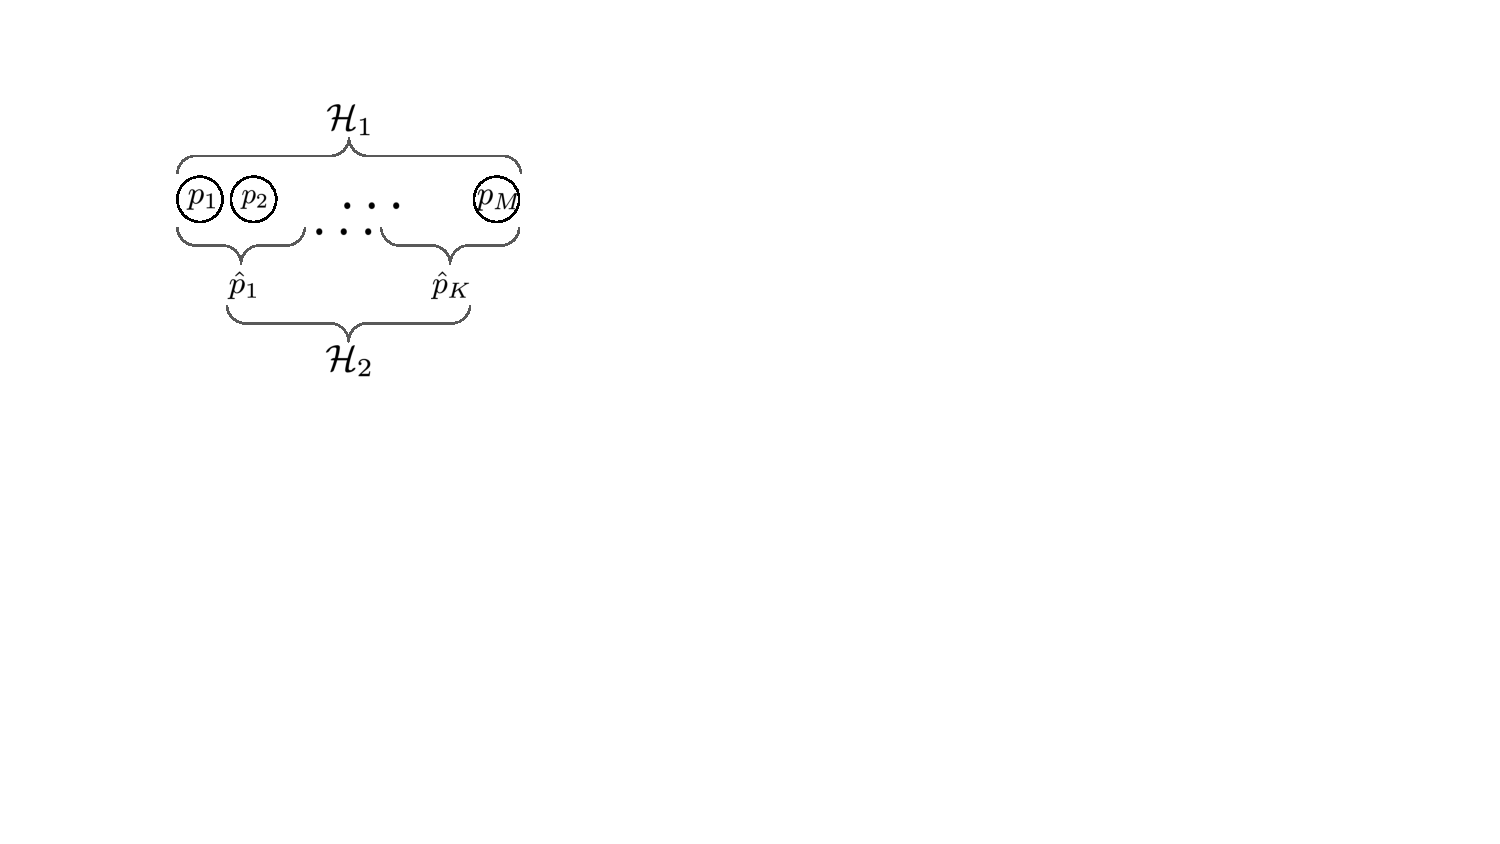
\includegraphics[width=0.3\linewidth]{pics/composability_H.pdf}
    \caption{Invariance of the entropy w.r.t. grouping events into disjoint sets.}
    \label{fig:composability_H}
\end{figure}

Let's consider a distribution $\{p_1,\ldots,p_M\}$, where the probabilities are given as rational numbers
\begin{align}
    p_i = \frac{m_i}{\sum_{j=1}^M m_j}\,.
\end{align}
Let's `ungroup' every event $x_i$ into $m_i$ events with uniform probabilities and use the invariance axiom
\begin{align}
    \ent(\{p_1,\ldots,p_M\}) + \sum_{i=1}^M p_i\ent(\{1/m_i,\ldots,1/m_i\}) = \ent(\{1/\sum_{i=1}^M m_i,\ldots,1/\sum_{i=1}^M m_i\})\,.
    \label{eq:rational_groups}
\end{align}
It's useful to introduce the following function
\begin{align}
    A(M) \coloneqq \ent(\{1/M,\ldots,1/M\})\,,
\end{align}
and note that, for $m_i = m\,,\;\forall i$, \cref{eq:rational_groups} becomes
\begin{align}
    A(M) + \sum_{i=1}^M \frac{m}{mM} A(m) = A(mM)\\
    A(M) + A(m) = A(mM)\,.
\end{align}
Clearly, for $m=1$,
\begin{align}
    A(M) + A(1) = A(M) \implies A(1) = 0\,.
\end{align}
For $m=M$,
\begin{align}
    A(m) + A(m) = A(m^2) \implies nA(m) = A(m^n)\,.
\end{align}
Thus, we see that $A(m) = \log m$ and using \cref{eq:rational_groups}, we have
\begin{align}
    \ent(\{p_1,\ldots,p_M\}) = - \sum_{i=1}^M p_i\log n_i + \log \sum_{j=1}^M \log n_j\, = - \sum_{i=1}^M p_i\log p_i\,.
\end{align}
This motivates the following definition.

\begin{mybox}
\begin{definition}[Entropy]\label{def:entropy}
    For a distribution over discrete outcomes $\{1,\ldots,M\}$ with probabilities $\{p_1,\ldots,p_M\}$, entropy is defined as
    \begin{align}
        \ent(\{p_1,\ldots,p_M\}) = -\sum_{i=1}^M p_i \log p_i\,.
    \end{align}
\end{definition}
\end{mybox}

Once we introduce the measure of uncertainty, or the measure of information, we can start asking questions about the distributions with the most uncertainty or the least information.
For example, consider a dataset $\mathcal{D}$ of observations $\{x_i\}_{i=1}^N$, and the statistics $u_k(x)$ evaluated on it, i.e.
\begin{align}
    \mean_{x\sim \mathcal{D}} u_k(x) = \frac{1}{N}\sum_{i=1}^N u_k(x_i) = \mu_k\,, \;\; k = 1,\ldots,K\,.
\end{align}
Then we can look for \textit{the distribution that explains the data and doesn't explain anything else}, as defined in the following definition.

\begin{mybox}
\begin{definition}[Maximum entropy principle]\label{def:max_ent}
    For the dataset $\mathcal{D}$ with statistics $\mu_k$, the maximum entropy principle defines the distribution as a solution to the following optimization problem
    \begin{align}
        \max_{p} \ent(\{p_1,\ldots,p_M\})\,, \;\; \text{ s.t. }\;\; \sum_{i=1}^M p_i u_k(i) = \mu_k\,, k = 1,\ldots,K\,.
    \end{align}
\end{definition}
\end{mybox}
Let's find the solution of this optimization problem.
First, the Lagrangian corresponding to the constrained optimization problem is
\begin{align}
    \mathcal{L}(\lambda, p) =~& \ent(\{p_1,\ldots,p_M\}) + \sum_{k=1}^K\lambda_k\left(\sum_{i=1}^M p_i u_k(i) - \mu_k\right) \\
    =~& -\sum_{i=1}^M p_i \log p_i + \sum_{k=1}^K\lambda_k\left(\sum_{i=1}^M p_i u_k(i) - \mu_k\right)\,.
\end{align}
We have to solve
\begin{align}
    \min_\lambda \max_p \mathcal{L}(\lambda, p)\,.
\end{align}
Taking the derivative w.r.t. $p$, we have
\begin{align}
    \deriv{\mathcal{L}}{p_j} = -\log p_j - 1 + \sum_k \lambda_k u_k(j) = 0 \implies p_j \propto \exp\left(\sum_k \lambda_k u_k(j)\right)\,,\\
    p_j = \frac{1}{Z_\lambda} \exp\left(\sum_k \lambda_k u_k(j)\right)\,, \;\; Z_\lambda = \sum_{j}^{M} \exp\left(\sum_k \lambda_k u_k(j)\right)\,.
\end{align}
Thus, we have
\begin{align}
    \min_\lambda \max_p \mathcal{L}(\lambda, p) =~& \min_\lambda \log Z_\lambda - \sum_{i=1}^M p_i \sum_k \lambda_k u_k(i) + \sum_{k=1}^K\lambda_k\left(\sum_{i=1}^M p_i u_k(i) - \mu_k\right)\\
    =~& \min_\lambda -\mean_{x\sim \mathcal{D}} \left[\sum_{k=1}^K \lambda_k u_k(x)-\log Z_\lambda\right] = \max_\lambda \mean_{x\sim \mathcal{D}} \log p_x\,,
\end{align}
which, as we see, is equivalent to maximum likelihood in the exponential family.

The same reasoning applies for the continuous random variables as follows.
\begin{mybox}
\begin{definition}[Differential Entropy]\label{def:diff_entropy}
    For a continuous random variable with the density $q(x)$, differential entropy is defined as
    \begin{align}
        \ent(q) = -\int dx\; q(x) \log q(x) = -\mean_{q(x)}\log q(x)\,.
    \end{align}
\end{definition}    
\end{mybox}
Let's see what the maximum entropy principle tells us for the differential entropy.
\begin{align}
    \max_{q} \ent(q(x))\,, \;\; \text{ s.t. }\;\; \int dx\; q(x)u_n(x) = \mu_n\,, n = 1,\ldots,N\,.
\end{align}
The Lagrangian corresponding to the problem is
\begin{align}
    \mathcal{L}(q,\lambda) =~& \ent(q) + \sum_{n=1}^N\lambda_n \left(\int dx\; q(x)u_n(x) - \mu_n\right) \\
    =~& -\int dx\;q(x)\log q(x) + \sum_{n=1}^N\lambda_n \left(\int dx\; q(x)u_n(x) - \mu_n\right)\,,
\end{align}
and the dual optimization problem is
\begin{align}
    \min_\lambda \max_q \mathcal{L}(q,\lambda)\,.
\end{align}
Let's write down the extremum condition for the inner optimization problem $\min_q \mathcal{L}(q,\lambda)$
\begin{align}
    \frac{\delta \mathcal{L}}{\delta q} = -\log q(x) + \sum_n\lambda_n u_n(x) = 0 \implies q(x) \propto \exp\left(\sum_n\lambda_n u_n(x)\right)\,.
\end{align}
From the normalization condition, we have
\begin{align}
    q(x\cond \lambda) = \frac{1}{Z_\lambda}\exp\left(\sum_n\lambda_n u_n(x)\right)\,,\;\; Z_\lambda = \int dx\; \exp\left(\sum_n\lambda_n u_n(x)\right)\,.
\end{align}
\begin{align}
    \mathcal{L}(q,\lambda) =~& \log Z_\lambda - \int dx\;q(x\cond \lambda)\left(\sum_n\lambda_n u_n(x)\right) + \sum_{n=1}^N\lambda_n \left(\int dx\; q(x\cond \lambda)u_n(x) - \mu_n\right) \\
    =~& \log Z_\lambda -\sum_{n=1}^N\lambda_n\mu_n = \log Z_\lambda -\sum_{n=1}^N\lambda_n\mean_{x \sim \mathcal{D}}\mu_n(x) = -\mean_{x \sim \mathcal{D}}\log q(x\cond \lambda)\,.
\end{align}
Thus, we have the following optimization problem
\begin{align}
    \min_\lambda \max_q \mathcal{L}(q,\lambda) = \min_\lambda - \log q(\mathcal{D}\cond \lambda) = \max_\lambda \log q(\mathcal{D}\cond \lambda)\,,
\end{align}
and we can make the following statement.

\begin{theorem}
    Maximum entropy principle corresponds to the maximum likelihood in the exponential family.
\end{theorem}

\begin{exercise}
    Find the density $q(x)$ of the random variable defined on $x \geq 0$ that has the biggest entropy and a given expectation $\mu$\,.
\end{exercise}

\begin{exercise}
    Find the density $q(x)$ of the random variable defined on $x \in \mathbb{R}$ that has the biggest entropy, given expectation $\mu$, and given variance $\sigma^2$\,.
\end{exercise}

\subsection{Bayesian Model Selection}
Design of the probabilistic model is the first step of Bayesian reasoning and oftentimes the choice of the model is not obvious.
We considered the priors that give us answers that are easy to compute, but what if a different prior fits better our purposes or which parameters of the prior should we choose? 
Let's look how the Bayesian inference looks like if we introduce model variable $m$ which we use to control the choice of the prior distribution (could the functional form or its parameters or both), i.e.
\begin{align}
    p(\theta\cond \mathcal{D}, m) = \frac{p(\mathcal{D}\cond\theta)p(\theta\cond m)}{p(\mathcal{D}\cond m)}\,.
\end{align}
Note that the denominator, which we usually refer to as a normalization constant of the posterior, i.e.
\begin{align}
    p(\mathcal{D}\cond m) = \int d\theta\;p(\mathcal{D}\cond\theta)p(\theta\cond m)\,,
\end{align}
is actually a likelihood of $m$ (indeed, it is the conditional distribution of the observed data $\mathcal{D}$ for model $m$).
Then we can choose the model according to the maximum likelihood principle (see \cref{def:mle}), i.e.
\begin{align}
    m_{\text{MLE}} = \argmax_m \underbrace{p(\mathcal{D}\cond m)}_{\text{evidence}}\,,
\end{align}
where the quantity $p(\mathcal{D}\cond m)$ is called \textit{evidence}.
After choosing the model, we can define our posterior distribution as
\begin{align}
    p(\theta\cond \mathcal{D}, m_{\text{MLE}})\,.
\end{align}

Alternatively, one can do the Bayesian inference on the model variable \kir{indeed, Bayesian inference is a way of reasoning, which can be applied to any variables. we can keep on doing this hierarchical inference any number of times}.
That is, we assume the uniform distribution over models $p(m) = \text{Uniform}[M]$ (let's say we have $M$ different models) \kir{of course, we can introduce more complicated priors}.
Then the posterior is the marginalization over $m$, i.e.
\begin{align}
    p(\theta\cond \mathcal{D}) = \sum_m p(\theta, m\cond \mathcal{D}) = \sum_m p(\theta\cond \mathcal{D}, m)p(m\cond \mathcal{D})\,, \;\;\text{ where }\;\; p(m\cond \mathcal{D}) \propto p(\mathcal{D}\cond m)p(m) \propto p(\mathcal{D}\cond m)\,.
\end{align}
Note that the posterior becomes the mixture of posteriors under different models $m$ weighted proportionally to their evidence $p(\mathcal{D}\cond m)$.

\begin{example}[Model selection]
    \label{example:model_selection}
    Consider three random variables $X,Y,Z$ which joint observations are given in the following table.\\
    \begin{center}
    \begin{tabular}{c|cc|cc}
        & \multicolumn{2}{c}{$x=0$} & \multicolumn{2}{c}{$x=1$}\\
         & $z=0$ & $z=1$ & $z=0$ & $z=1$ \\
        \midrule
        $y=0$ & $132$ & $19$ & $52$ & $11$ \\
        $y=1$ & $9$ & $0$ & $97$ & $6$
    \end{tabular}
    \end{center}
\end{example}

\begin{figure}[t]
    \centering
    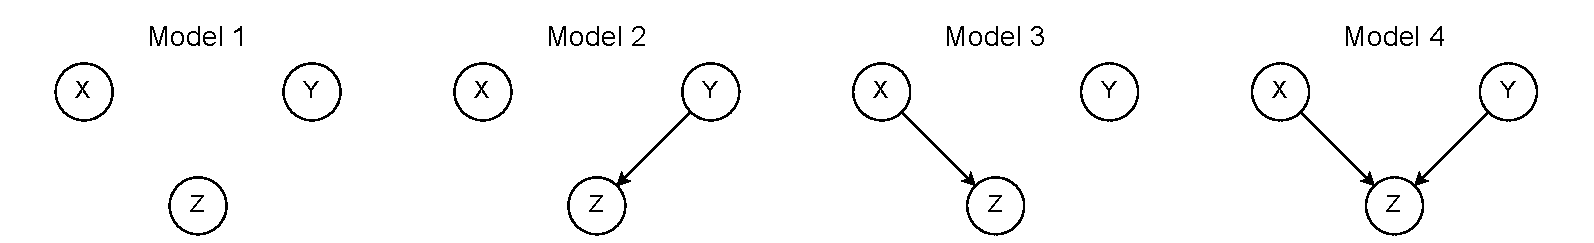
\includegraphics[width=0.95\textwidth]{pics/xyz_models.pdf}
    \caption{Models for \cref{example:model_selection}.}
    \label{fig:xyz_models}
\end{figure}



\subsection{Bayesian Linear Regression}

Let's consider the classical ML example --- linear regression.
The likelihood for linear regression is given as follows
\begin{align}
    p(y\cond x, \theta) = \Normal(y\cond w^Tx, \beta^{-1}) = \sqrt{\frac{\beta}{2\pi}}\exp\left(-\frac{\beta}{2}(y-w^Tx)^2\right)\,.
\end{align}
It's useful to think in terms of the log-likelihood, though, i.e.
\begin{align}
    \log p(y\cond x, \theta) = \log\Normal(y\cond w^Tx, \beta^{-1}) = -\frac{\beta}{2}(y- w^Tx)^2 + \frac{1}{2}\log \frac{\beta}{2\pi}\,.
\end{align}
First, let's find the maximum likelihood estimator $\theta_{\text{ML}} = \argmax_\theta \log p(\mathcal{D}\cond x, \theta)$ for the dataset $\mathcal{D} = \{(x_i,y_i)\}_{i=1}^N$.
That is, the derivative of the likelihood is
\begin{align}
    \nabla_w\sum_i\log\Normal(y_i\cond w^Tx_i, \beta^{-1}) = -\nabla_w\sum_i\frac{\beta}{2}(y_i- w^Tx_i)^2 = \beta\sum_i(y_i- w^Tx_i)x_i = 0\,,
\end{align}
where $x_i \in \mathbb{R}^d$ is a feature-vector of the $i$-th object.
It's convenient for us to introduce matrix $X$ such that $X_{ij}$ is the $j$-th coordinate of vector $x_i$ (of $i$-th object) and vector $y$ that consists of all the labels $y_i$.
Thus, we have
\begin{align}
    \sum_i y_iX_{ik} - \sum_i\sum_j w_{j} X_{ij} X_{ik} =~& 0\,, \;\forall\; k\,,\\
    X^Ty - X^TX w  =~& 0 \implies w_{\text{MLE}} = (X^TX)^{-1}X^Ty\,.
    \label{eq:linreg_mle}
\end{align}
Note that we got the classic formula for the linear regression.
Analogously, we have
\begin{align}
   \deriv{}{\beta}\left[\sum_i\log\Normal(y_i\cond w^Tx_i, \beta^{-1})\right] = -\sum_{i=1}^N\frac{1}{2}(y_i- w^Tx_i)^2 + \frac{N}{2\beta} = 0\\
   \frac{1}{\beta_{\text{MLE}}} = \frac{1}{N}\sum_{i=1}^N(y_i- w^Tx_i)^2 = \frac{1}{N}\norm{y-Xw}^2\,.
\end{align}

Now, let's introduce the prior distribution for the weights $w$.
That is, we assume that the weights are sampled (apriori) from the Normal distribution with the diagonal covariance matrix as follows
\begin{align}
    w \sim \Normal(w\cond 0,A^{-1})\,,\;\;\text{ where }\;\; 
    A = \begin{bmatrix}
        \alpha_1 & & 0\\
        & \ddots & \\
        0 & & \alpha_d
    \end{bmatrix}\,.
\end{align}
The posterior distribution for this model is defined as
\begin{align}
    p(\theta\cond \mathcal{D}) \propto \prod_{i=1}^N p(y_i\cond x_i,\theta) p(\theta) = \prod_{i=1}^N \Normal(y_i\cond w^Tx_i, \beta^{-1})\Normal(w\cond 0, A^{-1})\,.\\
    F(w) \coloneqq \prod_{i=1}^N \Normal(y_i\cond w^Tx_i, \beta^{-1})\Normal(w\cond 0, A^{-1})\,.
\end{align}
In this context, it is much easier to work with the logarithm of the density rather than with the density itself. Thus, we have
\begin{align}
    \log F(w) =~& \sum_{i=1}^N\log\Normal(y_i\cond w^Tx_i, \beta^{-1}) + \log\Normal(w\cond 0, A^{-1}) \\
    =~& -\sum_{i=1}^N\frac{\beta}{2}(y_i- w^Tx_i)^2 + \frac{N}{2}\log \frac{\beta}{2\pi} - \frac{1}{2}w^TAw + \frac{1}{2}\log \det(A) - \frac{d}{2}\log 2\pi\\
    =~& -\frac{\beta}{2}\norm{y-Xw}^2 + \frac{N}{2}\log \beta - \frac{1}{2}w^TAw + \frac{1}{2}\log \det(A) - \frac{d+N}{2}\log 2\pi\,.
\end{align}
Note that this a quadratic function, which means that the Taylor expansion of this function is going to contain only the first $3$ terms, i.e.
\begin{align}
    \log F(w) =~& \log F(w_{\text{MAP}}) + \inner{\nabla \log F(w_{\text{MAP}})}{w-w_{\text{MAP}}} + \\
    ~&+\frac{1}{2} (w - w_{\text{MAP}})^T \nabla^2_{ww} \log F(w_{\text{MAP}}) (w - w_{\text{MAP}}) + \underbrace{\deriv{^3}{w^3} + \ldots}_{=0}\,.
\end{align}
Note that we make the expansion at the point $w_{\text{MAP}}$ which is the Maximum A posteriori estimate, i.e.
\begin{align}
    w_{\text{MAP}} = \argmax_{w} \log F(w)\,.
\end{align}
Hence, $\nabla \log F(w_{\text{MAP}}) = 0$ is the necessary condition for being an optimum.
Thus, we have
\begin{align}
    \log F(w) =~& \log F(w_{\text{MAP}}) +\frac{1}{2} (w - w_{\text{MAP}})^T \nabla^2_{ww} \log F(w_{\text{MAP}}) (w - w_{\text{MAP}})\,.
\end{align}
Let's find $w_{\text{MAP}}$ first.
Clearly, we have
\begin{align}
    ~&\nabla_w \log F(w) = \beta X^T(y-Xw) - A w = 0\\
    ~&\beta X^Ty - \beta X^TX w - Aw  = 0 \implies w_{\text{MAP}} = \beta(\beta X^TX + A)^{-1}X^Ty = (X^TX + \beta^{-1}A)^{-1}X^Ty\,,
\end{align}
And the second derivative is
\begin{align}
    \nabla^2_{ww} \log F(w) = - \beta X^TX - A\,.
\end{align}

Remember that 
\begin{align}
    p(w\cond \mathcal{D}) \propto F(w) \implies \log p(w\cond \mathcal{D}) = \log F(w) + \text{const}\,,
\end{align}
where the constant can be defined from the normalization of the density (indeed, $p(w\cond \mathcal{D})$ has to be a valid density).
However, taking this integral is absolutely unnecessary since we already see that 
\begin{align}
    p(w\cond \mathcal{D}) \propto \exp\left( - \frac{1}{2} (w - w_{\text{MAP}})^T(\beta X^TX + A) (w - w_{\text{MAP}})\right)\,.
\end{align}
Thus, we have the following posterior distribution
\begin{align}
    p(w\cond \mathcal{D}) = \Normal\left(w\cond \underbrace{(X^TX + \beta^{-1}A)^{-1}X^Ty}_{w_{\text{MAP}}}, (\beta X^TX + A)^{-1}\right)\,.
\end{align}

Let's find the evidence
\begin{align}
    p(\mathcal{D}\cond \alpha,\beta) = \int dw\; p(\mathcal{D}\cond w,\beta)p(w\cond \alpha)\,.
\end{align}
Clearly, using the previously introduced notation, we have
\begin{align}
    p(\mathcal{D}\cond \alpha,\beta) =~& \int dw\; F(w) = F(w_{\text{MAP}})\int dw\; \exp\left[-\frac{1}{2} (w - w_{\text{MAP}})^T (\beta X^TX + A) (w - w_{\text{MAP}})\right]\\
    =~& F(w_{\text{MAP}}) \frac{(2\pi)^{d/2}}{\sqrt{\det(\beta X^TX + A)}}
\end{align}
Thus, we have to find $F(w_{\text{MAP}})$.
Let's do it
\begin{align}
    \log F(w_{\text{MAP}}) + \text{const} ~&= -\frac{\beta}{2}\norm{y-Xw_{\text{MAP}}}^2 - \frac{1}{2}w_{\text{MAP}}^TAw_{\text{MAP}}\\
    ~&= -\frac{\beta}{2}\left(y^Ty-2y^TXw_{\text{MAP}} + w_{\text{MAP}}^TX^TXw_{\text{MAP}} \right) - \frac{1}{2}w_{\text{MAP}}^TAw_{\text{MAP}}\\
    ~&= -\frac{\beta}{2}\left(y^Ty-2y^TXw_{\text{MAP}}\right) -\frac{1}{2} w_{\text{MAP}}^T\left(\beta X^TX + A\right)w_{\text{MAP}}\\
    ~&= -\frac{\beta}{2}\left(y^Ty-2\beta y^TX\left(\beta X^TX + A\right)^{-1} X^Ty\right) -\frac{\beta^2}{2} y^TX\left(\beta X^TX + A\right)^{-1} X^Ty\\
    ~&= -\frac{\beta}{2}y^T\left(I-\beta X\left(\beta X^TX + A\right)^{-1} X^T\right)y\\
    ~&= -\frac{\beta}{2}y^T\left(I- X\left(X^TX + \beta^{-1}A\right)^{-1} X^T\right)y
\end{align}
For the last expression, we need the Woodbury matrix identity
\begin{align}
    \left(A + UCV\right)^{-1} = A^{-1} - A^{-1}U\left(C^{-1} + VA^{-1}U\right)^{-1}VA^{-1}\,.
\end{align}
Thus, we have
\begin{align}
    \log F(w_{\text{MAP}}) = -\frac{\beta}{2}y^T\left(I + \beta^{-1}XA^{-1}X^T\right)^{-1}y + \frac{N}{2}\log \beta + \frac{1}{2}\log \det(A) - \frac{d+N}{2}\log 2\pi\,.
\end{align}
Finally, the evidence is
\begin{align}
    p(\mathcal{D}\cond \alpha,\beta) = \frac{(2\pi)^{d/2}\beta^{N/2}\sqrt{\det(A)}}{(2\pi)^{(d+N)/2}\sqrt{\det\left(\beta X^TX + A\right)}}\exp\left(-\frac{\beta}{2}y^T\left(I + \beta^{-1}XA^{-1}X^T\right)^{-1}y\right)\,,
\end{align}
for which, we can use
\begin{align}
    \det(A + UV) = \det(I + VA^{-1}U)\det(A)
\end{align}
and get
\begin{align}
    \beta^d\det\left(X^TX + \beta^{-1}A\right) = \beta^d\det(\beta^{-1}A)\det(I + \beta^{-1}XAX^T) = \det(A)\det(I + \beta^{-1}XAX^T)\,.
\end{align}
Thus, we have
\begin{align}
    p(\mathcal{D}\cond \alpha,\beta) = \frac{\beta^{N/2}}{(2\pi)^{N/2}\sqrt{\det(I + \beta^{-1}XAX^T)}}\exp\left(-\frac{\beta}{2}y^T\left(I + \beta^{-1}XA^{-1}X^T\right)^{-1}y\right)\,,
\end{align}
which we can then optimize as follows
\begin{align}
    \alpha^*,\beta^* = \argmax_{\alpha,\beta} p(\mathcal{D}\cond \alpha,\beta)\,.
\end{align}

To find the optimum of this function, it is easier to consider the variational bound of this function
\begin{mybox}
    \begin{definition}[Variational Bound]\label{def:var_bound}
    We call the function $g(x,\xi)$ a variational bound of function $f(x)$ if
    \begin{enumerate}
        \item $\forall \; x,\xi\;\; f(x) \geq g(x,\xi)\,,$
        \item $\forall \; x\; \exists\; \xi_x \; : f(x) = g(x,\xi_x)\,.$
    \end{enumerate}
    \end{definition}
\end{mybox}

\begin{align}
    \log p(\mathcal{D}\cond \alpha,\beta) =~& -\frac{\beta}{2}\norm{y-Xw_{\text{MAP}}}^2 - \frac{1}{2}w_{\text{MAP}}^TAw_{\text{MAP}} + \\
    ~&+ \frac{N}{2}\log \beta + \frac{1}{2}\log \det(A) - \frac{N}{2}\log 2\pi - \frac{1}{2}\log \det(\beta X^TX + A)\\
    \geq~& -\frac{\beta}{2}\norm{y-Xw}^2 - \frac{1}{2}w^TAw + \\
    ~&+ \frac{N}{2}\log \beta + \frac{1}{2}\log \det(A) - \frac{N}{2}\log 2\pi - \frac{1}{2}\log \det(\beta X^TX + A) \coloneqq \hat{F}(w,\alpha,\beta)
\end{align}

\begin{align}
    \deriv{}{w}\hat{F}(w,\alpha,\beta) = -\beta X^T(y - Xw) = 0 \implies w = w_{\text{MAP}}\,.
\end{align}

\begin{align}
    \deriv{}{\alpha_j}\hat{F}(w,\alpha,\beta) =~& -\frac{1}{2}w^2_j + \frac{1}{2}\frac{1}{\alpha_j} - \frac{1}{2} \inner{(\beta X^TX + A)^{-1}}{\deriv{}{\alpha_j}(\beta X^TX + A)} \\
    =~& -\frac{1}{2}w^2_j+ \frac{1}{2}\frac{1}{\alpha_j} - \frac{1}{2} (\beta X^TX + A)^{-1}_{jj} = 0\\
    \alpha_j =~& \frac{1}{w_j^2 + (\beta X^TX + A)^{-1}_{jj}}
\end{align}

\begin{align}
    \deriv{}{\beta}\hat{F}(w,\alpha,\beta) =~& -\frac{1}{2}\norm{y - Xw}^2 + \frac{N}{2\beta} - \frac{1}{2}\inner{(\beta X^TX + A)^{-1}}{\deriv{}{\beta}(\beta X^TX + A)}\\
    =~& -\frac{1}{2}\norm{y - Xw}^2 + \frac{N}{2\beta} - \frac{1}{2\beta}\inner{(\beta X^TX + A)^{-1}}{\beta X^TX \pm A}\\
    =~& -\frac{1}{2}\norm{y - Xw}^2 + \frac{N}{2\beta} - \frac{1}{2\beta}(d - \sum_j\alpha_j (\beta X^TX + A)^{-1}_{jj}) = 0\\
    \beta =~& \frac{N - d + \sum_j\alpha_j (\beta X^TX + A)^{-1}_{jj}}{\norm{y - Xw}^2}
\end{align}

\begin{exercise}
    Find the predictive distribution, i.e.
    \begin{align}
        p(y\cond x,\alpha,\beta)= \int dw\; \Normal(y\cond w^Tx, \beta^{-1})p(w\cond \mathcal{D}) = ?
    \end{align}
\end{exercise}

\subsection{Bayesian Logistic Regression, Laplace Approximation}

Consider the Logistic Regression for classification problem $y \in \{-1,1\}$
\begin{align}
    p(y\cond x,w) = \frac{1}{1+\exp(-yw^Tx)}
\end{align}
With the normal prior
\begin{align}
    p(w) = \Normal(w\cond 0, A^{-1})\,,\;\;\text{ where }\;\; 
    A = \begin{bmatrix}
        \alpha_1 & & 0\\
        & \ddots & \\
        0 & & \alpha_d
    \end{bmatrix}\,.
\end{align}

The posterior distribution is
\begin{align}
    p(w\cond \mathcal{D}) \propto \prod_i p(y_i\cond x_i,w) \Normal(w\cond 0, A^{-1})
\end{align}
\begin{align}
    \log p(w\cond \mathcal{D}) + \log Z =~& \sum_i \log p(y_i \cond x_i, w) - \frac{1}{2}w^TAw + \frac{1}{2} \log \det (A) - \frac{d}{2}\log (2\pi) \\
    =~& -\sum_i \log (1+\exp(-y_iw^Tx_i)) - \frac{1}{2}w^TAw + \frac{1}{2} \log \det (A) - \frac{d}{2}\log (2\pi) \coloneqq \log F(w)\,.
\end{align}
Let's do the same expansion as we did for the linear regression
\begin{align}
    \log F(w) =~& \log F(w_{\text{MAP}}) + \inner{\nabla \log F(w_{\text{MAP}})}{w-w_{\text{MAP}}} + \\
    ~&+\frac{1}{2} (w - w_{\text{MAP}})^T \deriv{^2}{w^2} \log F(w_{\text{MAP}}) (w - w_{\text{MAP}}) + \underbrace{\deriv{^3}{w^3} + \ldots}_{\neq 0}\,.
\end{align}
The last terms are not zero anymore, but this is an approximation.
Even for this, it's not trivial to find $w_{\text{MAP}}$
\begin{align}
    \nabla_w \log F(w) =~& -\sum_i \frac{\exp(-y_iw^Tx_i)}{1+\exp(-y_iw^Tx_i)}(-y_ix_i) - Aw = \sum_i \frac{1}{1+\exp(y_iw^Tx_i)}y_ix_i - Aw\\
    \deriv{^2}{w^2} \log F(w) =~& -\sum_i \frac{\exp(y_iw^Tx_i)}{(1+\exp(y_iw^Tx_i))^2}x_i x_i^T - A = -X^TR(w)X - A\,,
\end{align}
where $R(w)$ is the diagonal matrix with the elements
\begin{align}
    R(w)_{ii} = \frac{\exp(y_iw^Tx_i)}{(1+\exp(y_iw^Tx_i))^2}\,.
\end{align}
Thus, we approximate the posterior distribution as follows 
\begin{align}
    p(w\cond D) \propto F(w) \propto \Normal(w\cond w_{\text{MAP}}, (X^TR(w_{\text{MAP}})X + A)^{-1})\,.
\end{align}
Of course, this approximation is not specific to the logistic regression but a general technique that can be summarized as follows.
\begin{mybox}
\begin{definition}[Laplace approximation]
\label{def:laplace}
    For a given density $p(x)$ the Laplace approximation is 
    \begin{align}
        p(x) \approx \Normal(x\cond \mu, \Sigma)\,,\; \mu = \argmax_x p(x)\,,\;\; \Sigma^{-1} = -\nabla^2_{xx}\log p(x)\,.
    \end{align}
\end{definition}    
\end{mybox}


\begin{align}
    p(\mathcal{D}\cond A) = \int dw\; \prod_i p(y_i\cond x_i,w) \Normal(w\cond 0, A^{-1})
\end{align}

\clearpage
\section{Bayesian Variational Inference}
\label{sec:var_inference}

\subsection{Kullback-Leibler divergence}
The philosophy of the Bayesian variational inference is "if we cannot find the distribution analytically because it is too complicated, let us approximate it with a simpler distribution by minimizing some notion of discrepancy between distributions."

There are numerous ways for measuring discrepancy or divergence between distributions and all of them have their pros and cons. 
One of the most important ways comes from the information theory and is defined as follows.
\begin{mybox}
\begin{definition}[Kullback-Leibler divergence]\label{def:kl_div}
    For two discrete distributions $p$ and $q$ defined on the same set of outcomes $\{1,\ldots,M\}$, the Kullback-Leibler (KL) divergence is defined as
    \begin{align}
        \KL(p,q) = \sum_{i=1}^M p_i \log \frac{p_i}{q_i}\,.
    \end{align}
    Analogously, for two densities $p(x)$ and $q(x)$, and $x \in \Omega$, we have
    \begin{align}
        \KL(p(x),q(x)) = \int_\Omega dx\; p(x)\log \frac{p(x)}{q(x)}\,.
    \end{align}
\end{definition}    
\end{mybox}
\kir{it is tightly related to the concept of entropy and can be interpreted as the number of excess bits required for encoding the distribution $p(x)$ with the distribution $q(x)$.}

One can easily see that the KL-divergence is always positive
\begin{align}
    \KL(p(x),q(x)) =~& \int_\Omega dx\; p(x)\log \frac{p(x)}{q(x)}\\
    =~& -\int_\Omega dx\; p(x)\log \frac{q(x)}{p(x)}\\
    \geq~& -\log\left(\int_\Omega dx\; p(x) \frac{q(x)}{p(x)}\right) = -\log 1 = 0\,,
\end{align}
where we used the Jensen's inequality for probabilities.
Namely, for any convex function $f(x)$ and any function $\varphi(x)$, we have
\begin{align}
    \int dx\; p(x) f(\varphi(x)) \geq f\left(\int dx\; p(x)\varphi(x)\right)\,.
\end{align}
Furthermore, if $q(x) = p(x)$ it equals zero, indeed
\begin{align}
    \KL(p(x),p(x)) = \int_\Omega dx\; p(x)\log \frac{p(x)}{p(x)} = \int_\Omega dx\; p(x)\log 1 = \log 1 = 0\,.
\end{align}
Finally, one can prove that if $\KL(p(x),q(x)) = 0$ then $p(x) = q(x)$\,.

\begin{example}\label{example:variational_mle}
    Assume we observe some data $\mathcal{D} = \{x_1,\ldots, x_N\}$ that was generated from the distribution $x \sim p(x)$.
    Let's approximate $p(x)$ by solving
    \begin{align}
        \theta^* = \argmin_\theta \KL(p(x),q(x\cond\theta))\,.
    \end{align}
    First, let's rewrite the KL-divergence as follows
    \begin{align}
        \KL(p(x),q(x\cond\theta)) = \int dx\; p(x)\log\frac{p(x)}{q(x\cond\theta)} = \int dx\; p(x)\log p(x) - \int dx\; p(x)\log q(x\cond\theta)\,.
    \end{align}
    Note that the first term does not depend on $\theta$. Thus, we have
    \begin{align}
        \argmin_\theta \KL(p(x),q(x\cond\theta)) = \argmin_\theta - \int dx\; p(x)\log q(x\cond\theta) = \argmax_\theta \mean_{x\sim p(x)} \log q(x\cond\theta)\,.
    \end{align}
    In other words, we see that minimizing $\KL(p(x),q(x\cond\theta))$ is equivalent to the maximum likelihood principle from \cref{def:mle}.
\end{example}
    
\begin{exercise}
    Find the KL-divergence between two multivariate Gaussians with the same covariance matrix but different expectations, i.e.
    \begin{align}
        \KL(\Normal(\mu_1,\Sigma), \Normal(\mu_2,\Sigma)) = ?
    \end{align}
\end{exercise}

\begin{exercise}[Mode covering/seeking behaviour]
    Find the mean of the normal distribution that minimizes the KL-divergence between a Gaussian and some density $p(x)$, i.e.
    \begin{align}
        \argmin_\mu \KL(p(x), \Normal(x\cond \mu,\Sigma)) = ?
    \end{align}
    How the problem changes if we flip the arguments of the KL-divergence, i.e. we consider
    \begin{align}
        \argmin_\mu \KL(\Normal(x\cond \mu,\Sigma),p(x)) = ?
    \end{align}
\end{exercise}

\begin{exercise}
    Prove
    \begin{align}
        \KL(q,p) \leq \chi^2(q,p)\,,\;\; \text{ where }\;\;\chi^2(q,p) = \mean_{p(x)} \left(\frac{q(x)}{p(x)}-1\right)^2\,.
    \end{align}
\end{exercise}

\begin{exercise}
    Prove that for any $p_1,q_1,p_2,q_2$ and $\alpha \in [0,1]$, we have
    \begin{align}
        \KL(\alpha q_1 + (1-\alpha)q_2,\alpha p_1 + (1-\alpha)p_2) \leq \alpha\KL(q_1,p_1) + (1-\alpha)\KL(q_2,p_2)\,.
    \end{align}
\end{exercise}

\subsection{Evidence Lower Bound (ELBO)}
Let's take any approximation $q(\theta)$ and evaluate the KL-divergence between this approximation and the posterior distribution.
First, we just write the definition of the KL-divergence and the definition of the posterior distribution, i.e.
\begin{align}
    \KL(q(\theta),p(\theta\cond \mathcal{D})) =~& \int d\theta\; q(\theta)\log\frac{q(\theta)}{p(\theta\cond \mathcal{D})} = \int d\theta\; q(\theta)\log\frac{q(\theta)p(\mathcal{D})}{p(\mathcal{D}\cond \theta)p(\theta)}\\
    =~& - \int d\theta\;q(\theta) \log p(\mathcal{D}\cond \theta) + \int d\theta\; q(\theta)\log\frac{q(\theta)}{p(\theta)} + \log p(\mathcal{D})\,.
\end{align}
This is what we want to minimize. 
However, usually people take few more steps, i.e.
\begin{align}
    \KL(q(\theta),p(\theta\cond \mathcal{D})) =~& - \mean_{q(\theta)} \log p(\mathcal{D}\cond \theta) + \KL(q(\theta),p(\theta))  + \log p(\mathcal{D})\\
    \log p(\mathcal{D}) =~&  \mean_{q(\theta)} \log p(\mathcal{D}\cond \theta) -\KL(q(\theta),p(\theta)) + \KL(q(\theta),p(\theta\cond \mathcal{D}))\label{eq:evidence}\\
    \log \underbrace{p(\mathcal{D})}_{\text{evidence}} \geq~& \underbrace{\mean_{q(\theta)} \log p(\mathcal{D}\cond \theta) -\KL(q(\theta),p(\theta))}_{\text{Evidence Lower Bound}}\,,
\end{align}
where the last transition follows from the positivity of the KL-divergence.

It's a good moment to recall \cref{def:var_bound} and see the following fact.
\begin{theorem}
    Evidence Lower Bound is a variational bound.
\end{theorem}
\begin{proof}
    Indeed, we already showed that 
    \begin{align}
        \forall\, \mathcal{D}\,, q(\theta)\, \quad \log p(\mathcal{D}) \geq~& \mean_{q(\theta)} \log p(\mathcal{D}\cond \theta) -\KL(q(\theta),p(\theta))\,.
    \end{align}
    Thus, we just have to show the second requirement for a variational bound.
    Namely, we have to show
    \begin{align}
        \forall\, \mathcal{D}\,, \exists\, q(\theta)\, : \log p(\mathcal{D}) =~& \mean_{q(\theta)} \log p(\mathcal{D}\cond \theta) -\KL(q(\theta),p(\theta))\,.
    \end{align}
    From \cref{eq:evidence}, we can easily see that the equality is achieved at $q(\theta) = p(\theta\cond \mathcal{D})$, i.e. by perfectly fitting the posterior.
    Then, we have
    \begin{align}
        \mean_{p(\theta\cond\mathcal{D})} \log p(\mathcal{D}\cond \theta) -\KL(p(\theta\cond\mathcal{D}),p(\theta)) ~&= \int d\theta\; p(\theta\cond\mathcal{D}) \log\frac{p(\theta)p(\mathcal{D}\cond \theta)}{p(\theta\cond\mathcal{D})} \\
        ~&= \int d\theta\; p(\theta\cond\mathcal{D}) \log p(\mathcal{D}) =  \log p(\mathcal{D})\,.
    \end{align}
\end{proof}

Let's say we have parameterized the variational posterior $q(\theta\cond\varphi)$. 
Then, we can find the optimal parameters $\varphi^*$ by solving the following optimization problem
\begin{align}
    \varphi^* = \argmax_\varphi \mean_{q(\theta\cond \varphi)} \log p(\mathcal{D}\cond \theta) -\KL(q(\theta\cond \varphi),p(\theta))\,,
\end{align}
i.e. by maximizing the Evidence Lower Bound.
Usually we choose $q(\theta\cond\varphi)$ and $p(\theta)$ such that the KL-divergence can be found in the analytic form.
However, the first term $\mean_{q(\theta\cond \varphi)} \log p(\mathcal{D}\cond \theta)$ always requires a numerical estimation of the gradient (in order to use the gradient-based optimization algorithms).
Thus, we have a question how de we estimate the gradient $\nabla_\varphi \mean_{q(\theta\cond \varphi)} f(\theta)$\,.

Taking the gradient w.r.t. the parameters of the distribution is a big problem in probabilistic modeling
\begin{align}
    \nabla_\varphi \mean_{q(x\cond \varphi)} f(x) = ?
\end{align}
We will consider two approaches to this. The first one is straightforward
\begin{align}
    \nabla_\varphi \mean_{q(x\cond \varphi)} f(x) =~& \int dx\; \nabla_\varphi q(x\cond \varphi) f(x) = \int dx\; q(x\cond \varphi) f(x) \nabla_\varphi \log q(x\cond \varphi) \\
    =~& \mean_{q(x\cond \varphi)} f(x) \nabla_\varphi \log q(x\cond \varphi)\,.
\end{align}
Thus, we get the \textbf{score function gradient estimator}.
Note that 
\begin{align}
    \mean_{q(x\cond \varphi)} \nabla_\varphi \log q(x\cond \varphi) = \int dx\; \nabla_\varphi q(x\cond \varphi) = \nabla_\varphi \int dx\; q(x\cond \varphi) = \nabla_\varphi 1 = 0\,.
\end{align}
Thus, we can introduce so-called \textbf{baseline} as follows
\begin{align}
    \nabla_\varphi \mean_{q(x\cond \varphi)} f(x) = \mean_{q(x\cond \varphi)} f(x) \nabla_\varphi \log q(x\cond \varphi) = \mean_{q(x\cond \varphi)} (f(x) - b) \nabla_\varphi \log q(x\cond \varphi)\,,
\end{align}
where $b \in \mathbb{R}$ is a constant w.r.t. $x$.
In practice, the average value of $f$ minimizes the variance of the estimator, i.e.
\begin{align}
    \nabla_\varphi \mean_{q(x\cond \varphi)} f(x) \simeq \frac{1}{N}\sum_{i=1}^N\left(f(x_i) - \frac{1}{N-1}\sum_{j=1, j\neq i}^Nf(x_j)\right)\nabla_\varphi \log q(x_i\cond \varphi)\,.
    \label{eq:score_baseline_estimator}
\end{align}
\begin{exercise}
    Prove that the estimator in \cref{eq:score_baseline_estimator} is unbiased.
\end{exercise}

The second approach assumes that we can reparameterize $q(x\cond \varphi)$ as follows
\begin{align}
    g(\eps; \varphi) \sim q(x\cond \varphi)\,, \text{ where } \eps \sim q(\eps)\,,
\end{align}
i.e. there exist some, usually very simple, density $q(\eps)$ that does not depend on parameters $\varphi$ and the corresponding diffeormorphism (differentiable one-to-one function) $g(\eps; \varphi)$ that maps samples from $q(\eps)$ to samples from $q(x\cond \varphi)$. Then, one can write
\begin{align}
    \mean_{q(x\cond \varphi)} f(x) =~& \mean_{q(\eps)} 
    f(g(\eps;\varphi))\\
    \nabla_\varphi\mean_{q(x\cond \varphi)} f(x) =~& \mean_{q(\eps)} \nabla_\varphi f(g(\eps;\varphi)) = \mean_{q(\eps)} \deriv{g(\eps;\varphi)}{\varphi}\nabla_x f(x)\bigg|_{x=g(\eps;\varphi)}\,.
\end{align}
This is called the \textbf{reparameterization trick} or the \textbf{pathwise gradient estimator}.

In general, the reparameterization trick, when possible, is always better than the score gradient estimator.
Intuitively, this can be explained by the fact that score estimator does not use any information about the gradients of the function $f(x)$ (which carry a lot of information if the function is smooth).

\subsection{Latent Variables, EM-algorithm}
\label{sec:em-algo}

Extending the state-space with additional variables is one of the fundamental ideas in many disciplines \kir{the best example illustrating this is presented in "Ordinary Differential Equations" by V.Arnold in the problem about two circular wagons}.
In our case, when parameterizing a distribution on the state-space $\mathcal{X}$, we can always write
\begin{align}
    \int dz\; p(x,z\cond \theta) = p(x\cond\theta)\,,
\end{align}
i.e. we introduce another state-space $\mathcal{Z}$ and introduce the joint distribution on $\mathcal{X}\times\mathcal{Z}$, then we say that our parameterization $p(x\cond \theta)$ is simply the marginal of the joint distribution.
\kir{note that there is infinitely many joint distributions on $\mathcal{X}\times\mathcal{Z}$ that have the marginal $p(x\cond\theta)$}
\begin{mybox}
\begin{definition}[Latent Variables]\label{def:latents}
    In probabilistic inference, the extended space $\mathcal{Z}$ is called the \textbf{latent space} and the variables in this space are called \textbf{latent variables}.
\end{definition}
\end{mybox}

In particular, one can define the joint distribution as follows
\begin{align}
    p(x,z\cond \theta) = p(x\cond z;\theta)p(z\cond \theta)\,,
\end{align}
i.e. by defining the distribution over $z \in \mathcal{Z}$ and the conditional distribution on $x \in \mathcal{X}$.
Then, applying the maximum likelihood principle, we get
\begin{align}
    \text{Log-Likelihood}(\theta) = \mean_{x\sim p_{\text{data}}(x)}\log p(x\cond\theta) = \mean_{x\sim p_{\text{data}}(x)}\log \left[\mean_{z \sim p(z\cond\theta)}p(x\cond z;\theta)\right]\,.
\end{align}
This, however, is very hard to optimize because we usually can't estimate numerically the logarithm of the expectation.
Let's apply the variational principle to this.
Recall that in \cref{example:variational_mle} we derive the variational formulation of maximum likelihood as the miminization of the KL-divergence.
Let's apply the same technique, but for the joint distribution $p(x,z\cond \theta)$.
The obvious problem here is that we don't have the data distribution for the latent variables $z$, so let's use the posterior $p(z\cond x;\theta)$ of our model $p(x\cond z;\theta)p(z\cond \theta)$.
That is
\begin{align}
    \KL(p_{\text{data}}(x)p(z\cond x;\theta), p(x,z\cond \theta)) =~& \int dxdz\;p_{\text{data}}(x)p(z\cond x;\theta) \log\frac{p_{\text{data}}(x)p(z\cond x;\theta)}{p(x,z\cond \theta)}\\
    =~&  \int dxdz\;p_{\text{data}}(x)p(z\cond x;\theta) \log\frac{p_{\text{data}}(x)}{p(x\cond \theta)} = \KL(p_{\text{data}}(x),p(x\cond \theta))\,.
    \label{eq:variational_mle_extended}
\end{align}
Thus, we have that the minimization of the KL on the extended space is equivalent to maximum likelihood if we ``impute'' the latent variables of the target data with the posterior distribution.
The last step in this sequence is that we would like to get rid of the differentiation through the ``imputed'' latent variables by introducing the variational upper bound.
Namely, let's say we take some other posterior for generating the latents of the data, i.e. instead of $\KL(p_{\text{data}}(x)p(z\cond x;\theta), p(x,z\cond \theta))$, we consider 
\begin{align}
    \KL(p_{\text{data}}(x)~&\underbrace{p(z\cond x;\eta)}_{\text{different parameters!}}, p(x,z\cond \theta)) = \int dxdz\;p_{\text{data}}(x)p(z\cond x;\eta) \log \frac{p_{\text{data}}(x)p(z\cond x;\eta)}{p(x,z\cond \theta)}\\
    =~& \int dxdz\;p_{\text{data}}(x)p(z\cond x;\eta) \log \frac{p_{\text{data}}(x)}{p(x\cond \theta)} + \int dxdz\;p_{\text{data}}(x)p(z\cond x;\eta) \log \frac{p(z\cond x;\eta)}{p(z\cond x;\theta)}\\
    =~& \KL(p_{\text{data}}(x),p(x\cond \theta)) + \mean_{p_{\text{data}}(x)}\KL(p(z\cond x;\eta),p(z\cond x;\theta))\\
    =~& \KL(p_{\text{data}}(x)p(z\cond x;\theta), p(x,z\cond \theta)) + \mean_{p_{\text{data}}(x)}\underbrace{\KL(p(z\cond x;\eta),p(z\cond x;\theta))}_{\geq 0}\,,
\end{align}
where in the last transition we use \cref{eq:variational_mle_extended}.
Thus, we have derived the following variational upper bound
\begin{align}
\begin{split}
    \forall\; \theta\,,\eta\,,\;\;\KL(p_{\text{data}}(x)p(z\cond x;\theta), p(x,z\cond \theta)) \leq \KL(p_{\text{data}}(x)p(z\cond x;\eta), p(x,z\cond \theta))\,,\\
    \forall\; \theta\,,\;\exists \eta = \theta \,,\;\;\KL(p_{\text{data}}(x)p(z\cond x;\theta), p(x,z\cond \theta)) = \KL(p_{\text{data}}(x)p(z\cond x;\eta), p(x,z\cond \theta))\,.
    \label{eq:em_variational_bound}
\end{split}
\end{align}
Thus, we have proved the following result.
\begin{proposition}[Variational Formulation of the EM-algorithm]
The following optimization problems are equivalent
    \begin{align}
        \max_\theta \mean_{x\sim p_{\text{data}}(x)}\log \left[\mean_{z \sim p(z\cond\theta)}p(x\cond z;\theta)\right] \iff \min_\theta \min_\eta\KL(p_{\text{data}}(x)p(z\cond x;\eta), p(x,z\cond \theta))\,.
    \end{align}
\end{proposition}

\begin{mybox}
\begin{definition}[EM-algorithm]\label{def:em_algo}
    The iterative optimization of the following variational upper bound w.r.t. $\eta$ and $\theta$ is called the Expectation Maximization (EM) algorithm
    \begin{align}
        \KL(p_{\text{data}}(x)p(z\cond x;\theta), p(x,z\cond \theta)) \leq \KL(p_{\text{data}}(x)p(z\cond x;\eta), p(x,z\cond \theta))\,.
    \end{align}
\end{definition}    
\end{mybox}

\paragraph{Expectation step (E-step)} is the optimization w.r.t. the parameters $\eta$. This optimization problem is trivial due to the variational bound above. Indeed, simply setting $\eta = \theta$ minimizes the bound.
That is why, oftentimes, people say that at the E-step we find the posterior distribution
\begin{align}
    p(z\cond x_i;\theta)\,,\;\; x_i \sim p_{\text{data}}(x)\,,
\end{align}
which then we can use to estimate the objective by integrating w.r.t. $z$ or sampling the latent variables
\begin{align}
    z_i \sim p(z\cond x_i;\theta)\,,\;\; x_i \sim p_{\text{data}}(x)\,.
\end{align}

\paragraph{Maximization step (M-step)} is the \textit{minimization} of the derived variational upper bound on the KL-divergence w.r.t. $\theta$, i.e.
\begin{align}
    \theta^* = \argmin_\theta \KL(p_{\text{data}}(x)p(z\cond x;\eta), p(x,z\cond \theta))\,.
\end{align}

Well, why do people call it the maximization step then? It's very simple --- there is another interpretation of this optimization problem.
Recall \cref{eq:variational_mle_extended}, then we can write 
\begin{align}
    \KL(p_{\text{data}}(x), p(x\cond \theta)) \leq~& \KL(p_{\text{data}}(x)p(z\cond x;\eta), p(x,z\cond \theta))\\
    \mean_{p_{\text{data}}(x)}\left[\log p_{\text{data}}(x) - \log p(x\cond \theta)\right] \leq~& \mean_{p_{\text{data}}(x)p(z\cond x;\eta)}\big[\log p_{\text{data}}(x) + \log p(z\cond x;\eta) \\
    ~&- \log p(x,z\cond \theta)\big]\\
     \mean_{p_{\text{data}}(x)p(z\cond x;\eta)}\left[-\log p(z\cond x;\eta) + \log p(x,z\cond \theta)\right]\leq~& \mean_{p_{\text{data}}(x)}\log p(x\cond \theta)\,.
\end{align}
Let's rearrange the terms on the left by decomposing the joint density $p(x,z\cond \theta) = p(x\cond z;\theta)p(z\cond \theta)$
\begin{align}
    \underbrace{\mean_{p_{\text{data}}(x)p(z\cond x;\eta)}\log p(x\cond z;\theta) - \mean_{p_{\text{data}}(x)}\KL(p(z\cond x;\eta),p(z\cond\theta))}_{\text{lower bound}}\leq~& \underbrace{\mean_{p_{\text{data}}(x)}\log p(x\cond \theta)}_{\text{marginal likelihood}}\,.
\end{align}
Namely, for the M-step, eliminating the terms that are independent of $\theta$, we have the following result.
\begin{proposition}[M-step]
The following optimization problems are equivalent
    \begin{align}
        \argmin_\theta \KL(p_{\text{data}}(x)p(z\cond x;\eta), p(x,z\cond \theta)) = \argmax_\theta \mean_{p_{\text{data}}(x)p(z\cond x;\eta)}\log p(x\cond z;\theta)p(z\cond\theta)\,.
    \end{align}
\end{proposition}

\subsection{Variational Auto-Encoder (VAE) \citep{kingma2013auto}}

Finding the posterior distribution $p(z\cond x;\theta)$ might be infeasible in practice.
Indeed, if the likelihood model is a neural network, e.g.
\begin{align}
    p(x\cond z;\theta) = \Normal(x\cond \mu(z;\theta), \sigma^2(z;\theta))\,,
\end{align}
where $\mu(z;\theta)$ and $\sigma^2(z;\theta))$ are outputs of the network, then finding $p(z\cond x;\theta)$ in closed form is impossible. 
Even sampling $z \sim p(z\cond x;\theta) \propto p(x\cond z;\theta)p(z\cond \theta)$ might be very complicated task.

The idea is to approximate $p(z\cond x;\theta)$ with another parametric model $q(z\cond x;\eta)$.
We already have all the necessary tools for this!
Indeed, when proving the variational bound \cref{eq:em_variational_bound} we did not use anywhere that the posterior with different parameters $\eta$ has the same functional family as the true posterior.
Thus, we can write the following
\begin{align}
    \KL(p_{\text{data}}(x)\underbrace{p(z\cond x;\theta)}_{\text{true posterior}}, p(x\cond z;\theta)p(z\cond \theta)) \leq \KL(p_{\text{data}}(x)\underbrace{q(z\cond x;\eta)}_{\text{approximation}}, p(x\cond z;\theta)p(z\cond \theta))\,,
\end{align}
i.e. instead of using the posterior from the same functional family but with different parameters (from the previous iteration) as in the EM-algorithm, we approximate the posterior with a completely independent model $q(z\cond x;\eta)$.
This is a variational bound in the following sense
\begin{align}
\begin{split}
    ~&\forall\; \theta\,,q(z\cond x;\eta)\,,\;\;\KL(p_{\text{data}}(x)p(z\cond x;\theta), p(x\cond z;\theta)p(z\cond \theta)) \leq \KL(p_{\text{data}}(x)q(z\cond x;\eta), p(x\cond z;\theta)p(z\cond \theta))\,,\\
    ~&\forall\; \theta\,,\;\exists q(z\cond x;\eta) = p(z\cond x;\theta) \,,\;\;\KL(p_{\text{data}}(x)p(z\cond x;\theta), p(x,z\cond \theta)) = \KL(p_{\text{data}}(x)p(z\cond x;\eta), p(x,z\cond \theta))\,.
    \label{eq:vae_variational_bound}
\end{split}
\end{align}
Clearly, the same result holds for the lower variational bound on the marginal log-likelihood, i.e.
\begin{align}
    \mean_{p_{\text{data}}(x)q(z\cond x;\eta)}\log p(x\cond z;\theta) - \mean_{p_{\text{data}}(x)}\KL(p(z\cond x;\eta),p(z\cond\theta))\leq~& \mean_{p_{\text{data}}(x)}\log p(x\cond \theta)\,.
\end{align}

\begin{exercise}[VAE with Gaussians]
    Consider the following parametric model
    \begin{align}
        \underbrace{p(x\cond z;\theta) = \Normal(x\cond \mu(z;\theta),\sigma^2(z;\theta))}_{\text{decoder}}\,,\;\;\underbrace{p(z\cond \theta) = \Normal(0,1)}_{\text{prior}}\,,\;\; \underbrace{q(z\cond x;\eta) = \Normal(z\cond \mu(x;\eta),\sigma^2(x;\eta))}_{\text{encoder}}\,.
    \end{align}
    For this model, write down the training objective for both the encoder and the decoder, i.e. the KL upper bound or the log-likelihood lower bound. Which integrals you can take and which of them you have to estimate via Monte Carlo? Which gradient estimator you should use to estimate the gradients w.r.t. $\theta$ and $\eta$?
\end{exercise}

\subsection{Importance Weighted Auto-Encoder (IWAE) \citep{burda2015importance}}

The log-likelihood lower bound is usually derived in the following way.
First, one uses the definition of the marginal density and introduce a fictional density $q$, which can be anything, i.e.
\begin{align}
    p(x\cond \theta) = \int dz\; p(x, z\cond \theta) = \int dz\; q(z\cond x;\eta)\frac{p(x,z\cond\theta)}{q(z\cond x;\eta)}\,,\;\; \forall\; q(z\cond x;\eta)\,.
    \label{eq:vae_marginal_ll}
\end{align}
Then one can use the Jensen's inequality for the logarithm and get
\begin{align}
    \log p(x\cond \theta) \geq \int dz\; q(z\cond x;\eta)\log \frac{p(x,z\cond \theta)}{q(z\cond x;\eta)} = \mean_{q(z\cond x;\eta)}\log \frac{p(x,z\cond \theta)}{q(z\cond x;\eta)}\,,\;\; \forall\; q(z\cond x;\eta)\,.
\end{align}
When we do this there are 
\begin{itemize}[label={}]
    \item \yes good news: we get a lower bound on the log-likelihood amenable for optimization;
    \item \no bad news: the bound is tight only for the true posterior, i.e. $q(z\cond x;\eta) = p(z\cond x;\theta)$.
\end{itemize}
Note that the estimate in \cref{eq:vae_marginal_ll} holds for any $q$ and there is no bounds/errors introduced there yet. \kir{of course the problem of optimizing the marginal density directly is that the density is log-concave. for instance, consider the gaussian, the gradient of the density vanishes very fast once you go far from the mode. however, the gradient of the log-density is simply $x$ and does not vanish anywhere (formally, except the mode).}
This spurred the following idea, what if we could draw more samples in \cref{eq:vae_marginal_ll} first and only \textit{then} take the logarithm and use Jensen's inequality?
Indeed, we can write
\begin{align}
    p(x\cond \theta) ~&= \frac{1}{K}\sum_{i=1}^K\int dz_i\; p(x, z_i\cond \theta) = \frac{1}{K}\sum_{i=1}^K\int dz_i\; q(z_i\cond x;\eta)\frac{p(x,z_i\cond\theta)}{q(z_i\cond x;\eta)}\\
    ~&=\frac{1}{K}\sum_{i=1}^K\int \prod_{j=1}^K dz_j\; q(z_j\cond x;\eta)\frac{p(x,z_i\cond\theta)}{q(z_i\cond x;\eta)}=\int \prod_{j=1}^K dz_j\; q(z_j\cond x;\eta)\frac{1}{K}\sum_{i=1}^K\frac{p(x,z_i\cond\theta)}{q(z_i\cond x;\eta)}\,,
    \label{eq:iwae_marginal_ll}
\end{align}
i.e. we just ``copied'' the expression $K$ times and labeled the variables differently, which, of course, does not change the value of the expression. On the second row of derivations we use the fact that the integral expression depends only on $z_i$, so all the other densities over $z_j$ integrate to $1$. \kir{note that we could choose completely different densities $q^i(z_i\cond x;\eta_i)$ but we keep the same density for simplicity}
The final step is to take the logarithm and to apply Jensen's inequality, i.e.
\begin{align}
    \log p(x\cond \theta) \geq  \int \prod_{j=1}^K dz_j\; q(z_j\cond x;\eta)\log \frac{1}{K}\sum_{i=1}^K\frac{p(x,z_i\cond\theta)}{q(z_i\cond x;\eta)} = \mean_{z_1,\ldots,z_K \sim q}\log \frac{1}{K}\sum_{i=1}^K\frac{p(x,z_i\cond\theta)}{q(z_i\cond x;\eta)}\,.
\end{align}
Thus, we have derived the IWAE lower bound on the marginal density. This bound can be used to train or to evaluate auto-encoding models.

\begin{proposition}[IWAE estimator]
    The IWAE estimator of the marginal density is
    \begin{align}
        \log p(x\cond \theta) \geq \mean_{z_1,\ldots,z_K \sim q}\log \frac{1}{K}\sum_{i=1}^K\frac{p(x,z_i\cond\theta)}{q(z_i\cond x;\eta)}\,, \text{ where } z_i \sim q(z_i\cond x;\eta)\,.
    \end{align}
\end{proposition}

\begin{exercise}
    Prove that the bound becomes tighter with the number of samples $K$.
\end{exercise}

\subsection{Denoising Diffusion Probabilistic Models (DDPM) \citep{sohl2015deep}}

First, I would like to give a small motivation for introducing diffusion models. VAE had a tremendous success in the ML/DL community and quickly started spreading to other fields. It was very simple to understand, implement, and train while allowing for a qualitatively new level of generative modeling. Quickly, it was overshadowed by Generative Adversarial Networks (GANs), but always remained an actively studied/utilized model. Despite this, VAE had limitations, which were formalized as posterior collapse to the prior and ELBO not giving tight enough bounds etc.

\kir{Informally, there was a common intuition that you can't get a good density model by slapping a gaussian on top of network's output, and this fact was much more influential than all the mathematical arguments. That's why people started building hierarchical VAEs, i.e. putting a VAE inside a VAE.}

Following DDPM \citep{sohl2015deep, ho2020denoising} we define the density model as the marginal following backward (decoding) process
\begin{align}
\begin{split}
    \label{eq:backward_process}
    p(x_0\cond \theta) =~& \int dx_1,\ldots,dx_T\; p(x_T)\prod_{t=1}^Tp(x_{t-1}\cond x_t; \theta)\,, \\
    ~&\text{where } p(x_T) = \Normal(0,1)\,,\;\; p(x_{t-1}\cond x_t;\theta) = \Normal(x_{t-1}\cond \mu(x_t;\theta), g_t^2)\,.
\end{split}
\end{align}
After defining a density model we, as always, can write down the lower bound on the log-density as follows
\begin{align}
    \log p(x_0\cond \theta) ~&= \log \int dx_1\ldots dx_T\; p(x_T)\prod_{t=1}^{T} p(x_{t-1}\cond x_t;\theta) \\
    ~&= \log \int dx_1\ldots dx_T\; \prod_{t=1}^{T} q(x_{t}\cond x_{t-1})\frac{p(x_T)\prod_{t=1}^{T} p(x_{t-1}\cond x_t;\theta)}{\prod_{t=1}^{T} q(x_{t}\cond x_{t-1})}\\
    ~&\geq \mean_{\prod_{t=1}^{T} q(x_{t}\cond x_{t-1})} \log \frac{p(x_T)\prod_{t=1}^{T} p(x_{t-1}\cond x_t;\theta)}{\prod_{t=1}^{T} q(x_{t}\cond x_{t-1})} \\
    ~&= \mean_{\prod_{t=1}^{T} q(x_{t}\cond x_{t-1})}\left[ \log p(x_T) + \sum_{t=1}^{T} \log \frac{p(x_{t-1}\cond x_t;\theta)}{q(x_{t}\cond x_{t-1})}\right]\,.\label{eq:ddpm_lb}
\end{align}
Note that this holds for any forward (encoding) process $\prod_{t=1}^{T} q(x_{t}\cond x_{t-1})$. To progress further, we need to introduce the marginals of this process as follows
\begin{align}
    q(x_\tau \cond x_0)\coloneqq \int dx_{1}\ldots dx_{\tau-1}\; \prod_{t=1}^{\tau} q(x_{t}\cond x_{t-1})\,,\;\text{ and }\; q(x_0\cond x_0)\coloneqq 1\,.
\end{align}
Using this definition and the lower bound from \cref{eq:ddpm_lb}, we have
\begin{align}
    \log p(x_0\cond \theta) \geq~& \mean_{\prod_{t=1}^{T} q(x_{t}\cond x_{t-1})}\left[ \log p(x_T) + \sum_{t=1}^{T} \log \frac{p(x_{t-1}\cond x_t;\theta)}{q(x_{t}\cond x_{t-1})}\right]\\
    =~& \mean_{q(x_T\cond x_0)}\log p(x_T) + \sum_{t=1}^{T}\mean_{q(x_{t-1}\cond x_0)q(x_{t}\cond x_{t-1})}\log \frac{p(x_{t-1}\cond x_t;\theta)}{q(x_{t}\cond x_{t-1})}\,.
\end{align}
The final step in the derivation is to \textit{define} $q(x_{t-1}\cond x_t, x_0)$. Indeed, for the joint distribution $q(x_{t}\cond x_{t-1})q(x_{t-1}\cond x_0)$, we can define (using \cref{def:cond_dist}) the following conditional distribution
\begin{align}
    q(x_{t-1}\cond x_{t}, x_0) \coloneqq \frac{q(x_{t}\cond x_{t-1})q(x_{t-1}\cond x_0)}{\int dx_{t-1}\;q(x_{t}\cond x_{t-1})q(x_{t-1}\cond x_0)} = \frac{q(x_{t}\cond x_{t-1})q(x_{t-1}\cond x_0)}{q(x_t\cond x_0)}\,.
\end{align}
Continuing with this definition, we get
\begin{align}
    \log p(x_0\cond \theta) \geq~& \mean_{q(x_T\cond x_0)}\log p(x_T) - \sum_{t=1}^{T}\mean_{q(x_{t}\cond x_0)}\KL(q(x_{t-1}\cond x_{t},x_0),p(x_{t-1}\cond x_t;\theta)) + \\
    ~& + \sum_{t=1}^{T}\mean_{q(x_{t-1}\cond x_0)q(x_{t}\cond x_{t-1})}\log\frac{q(x_{t-1}\cond x_0)}{q(x_t\cond x_0)}\,.
\end{align}
For the last term, we have
\begin{align}
    \sum_{t=1}^{T}\mean_{q(x_{t-1}\cond x_0)q(x_{t}\cond x_{t-1})}\log\frac{q(x_{t-1}\cond x_0)}{q(x_t\cond x_0)} =~& \sum_{t=0}^{T-1}\mean_{q(x_{t}\cond x_0)}\log q(x_t\cond x_0) - \sum_{t=1}^{T}\mean_{q(x_{t}\cond x_0)}\log q(x_t\cond x_0)\\
    =~& \mean_{q(x_{0}\cond x_0)}\log q(x_0\cond x_0) - \mean_{q(x_{T}\cond x_0)}\log q(x_T\cond x_0) \\
    =~& - \mean_{q(x_{T}\cond x_0)}\log q(x_T\cond x_0)\,.
\end{align}
Finally, we have the following result
\begin{theorem}[Backward Process Lower Bound]
    For the backward process from \cref{eq:backward_process} and any forward process $q(x_{t}\cond x_{t-1})$, we have the following lower bound on the log-density
    \begin{align}
    \log p(x_0\cond \theta) \geq~& - KL(q(x_T \cond x_0),p(x_T)) - \sum_{t=1}^{T}\mean_{q(x_{t}\cond x_0)}\KL(q(x_{t-1}\cond x_{t},x_0),p(x_{t-1}\cond x_t;\theta))\,.
    \end{align}
\end{theorem}
\begin{proposition}[Variational formulation]
    For the backward process from \cref{eq:backward_process} and any forward process $q(x_{t}\cond x_{t-1})$, we can derive the following upper bound on the KL-divergence
    \begin{align}
    \KL(p_{\text{data}}(x_0), p(x_0\cond \theta)) \leq~&  KL(q(x_T),p(x_T)) + \sum_{t=1}^{T}\mean_{q(x_{t})}\KL(q(x_{t-1}\cond x_{t}),p(x_{t-1}\cond x_t;\theta))\,,
    \end{align}
    where $p_{\text{data}}(x_0)$ is the density of the data distribution and the marginals $q(x_\tau)$ are defined as
    \begin{align}
        q(x_\tau)\coloneqq \int dx_0\;q(x_\tau\cond x_0)p_{\text{data}}(x_0)\,.
    \end{align}
\end{proposition}
\begin{exercise}
    Derive the variational formulation.
\end{exercise}


Theoretically, using this lower bound on the log-likelihood or its variational formulation in terms of the KL, one could parameterize both $q$ and $p$ and solve the optimization problem w.r.t. the models' parameters. In practice, however, a naive parameterization of this does not work
\begin{itemize}[label={}]
    \item \no indeed, to get the marginal $q(x_\tau \cond x_0)$ one has to apply the parameteric model multiple times what creates a lot of numerical instabilities;
    \item \no furthermore, there exist infinite number of marginal sequences $q(x_\tau)$ between $p_{\text{data}}(x_0)$ and $p(x_T)$, hence, multiple forward and backward processes.
\end{itemize}

\cite{sohl2015deep} solved these problems by fixing the forward (encoding) process $q(x_t\cond x_{t-1})$ to the \textit{diffusion process}, which bears the following benefits
\begin{itemize}[label={}]
    \item \yes there is unique sequence of marginals $q(x_\tau)$, hence the marginals of the backward process are also fixed \kir{still exists infinitely many conditionals}.
    \item \yes sampling from $q(x_\tau \cond x_0)$ can be performed directly, i.e. without simulating multiple transition kernels $q(x_t\cond x_{t-1})$;
    \item \yes from physics we know that the functional form of the reverse (backward) process is the same as the forward diffusion process \citep{feller1949theory}. \kir{thus, for the first time in history, it was mathematically OK to slap a gaussian on networks' outputs.}
\end{itemize}
In particular, the diffusion process (its time discretization) is defined by the following forward transition kernel
\begin{align}
    q(x_t\cond x_{t-1}) = \Normal(x_t\cond \alpha_t x_{t-1}, \sigma_t^2 \mathds{1})\,,
\end{align}
that is, to generate next $x_t$ we have to scale $x_{t-1}$ by some scalar $\alpha_t$ and add some noise
\begin{align}
    x_t = \alpha_t x_{t-1} + \sigma_t \eps\,, \;\; \eps \sim\Normal(\eps\cond 0,1)\,.
\end{align}
For this process, we would like to find the following marginal
\begin{align}
    q(x_t\cond x_{0}) = ?
\end{align}
However, first, let's answer a simpler question $q(x_t\cond x_{t-2}) = ?$ That is,
\begin{align}
    x_t ~&= \alpha_t x_{t-1} + \sigma_t \eps = \alpha_t (\alpha_{t-1}x_{t-2} + \sigma_{t-1}\eps') + \sigma_t \eps\,, \;\;\eps,\eps'\sim \Normal(0,\mathds{1})\\
    ~&= \alpha_t \alpha_{t-1} x_{t-2} + \alpha_t\sigma_{t-1}\eps' + \sigma_t \eps\,.
\end{align}
Thus, we have
\begin{align}
    q(x_t\cond x_{t-2}) = \Normal(x_t\cond \alpha_t \alpha_{t-1} x_{t-2}, ((\alpha_t \sigma_{t-1})^2 + \sigma_t^2)\mathds{1})\,.
\end{align}
Applying this proposition iteratively, we get the following formula.
\begin{proposition}
    For the transition probability $q(x_t\cond x_{t-1}) = \Normal(x_t\cond \alpha_t x_{t-1}, \sigma_t^2 \mathds{1})$, we have the following formula for the marginals
    \begin{align}
        q(x_\tau\cond x_{0}) = \Normal\left(x_t\bigg| \prod_{t=1}^\tau\alpha_t x_{0}, \sum_{t=1}^\tau \sigma_t^2 \prod_{i=t+1}^\tau\alpha_i^2\mathds{1}\right)\,.
    \end{align}
\end{proposition}
To evaluate the objective we need the following conditional density.
\begin{exercise}
    For the transition probability $q(x_t\cond x_{t-1}) = \Normal(x_t\cond \sqrt{1-\beta_t} x_{t-1}, \beta_t \mathds{1})$, derive $q(x_{t-1}\cond x_{t}, x_0)$ using the definition
    \begin{align}
    q(x_{t-1}\cond x_{t}, x_0) \coloneqq \frac{q(x_{t}\cond x_{t-1})q(x_{t-1}\cond x_0)}{\int dx_{t-1}\;q(x_{t}\cond x_{t-1})q(x_{t-1}\cond x_0)} = \frac{q(x_{t}\cond x_{t-1})q(x_{t-1}\cond x_0)}{q(x_t\cond x_0)}\,.
    \end{align}
\end{exercise}
The final step is to derive the KL-divergence
\begin{exercise}
    For the transition probability $q(x_t\cond x_{t-1}) = \Normal(x_t\cond \sqrt{1-\beta_t} x_{t-1}, \beta_t \mathds{1})$ and parameterized model of the backward process $p(x_{t-1}\cond x_{t}) = \Normal(x_{t-1}\cond \mu_t(x_t;\theta), \beta_t \mathds{1})$, find
    \begin{align}
        \KL(q(x_{t-1}\cond x_{t}),p(x_{t-1}\cond x_t;\theta)) = ?
    \end{align}
\end{exercise}
\clearpage
\section{Monte Carlo methods}

Monte Carlo methods are usually used to numerically estimate the integrals of the form
\begin{align}
    \int dx\; p(x)f(x) = \mean_{p(x)} f(x)\,.
\end{align}
The key insight here is that instead of approximating the expression on the left using a regular grid or quadratures, one can draw samples distributed as $p(x)$ and approximate
\begin{align}
    \mean_{p(x)} f(x) \simeq \frac{1}{N}\sum_{i=1}^N f(x_i)\,, x_i \sim p(x)\,.
\end{align}
To understand the behaviour of this estimate one can use the Central Limit Theorem.
\begin{theorem}[Central Limit Theorem]
    Consider a random variable $X$ with the density $p(x)$, mean $\mu$, and variance $\sigma^2$. The following convergence result takes place
    \begin{align}
        \sqrt{n}(\hat{\mu}_n-\mu) \xrightarrow[]{d} \Normal(0,\sigma^2)\,, \;\; \hat{\mu}_n = \frac{1}{n}\sum_{i=1}^n x_i\,, x_i \sim p(x)\,,
    \end{align}
    where $\xrightarrow[]{d}$ denotes the convergence in distribution.
\end{theorem}
Using this estimator one can, for instance, estimate the predictive distribution of a Bayesian model as follows
\begin{align}
    \int d\theta\; p(x\cond \theta)p(\theta\cond \mathcal{D}) = \mean_{p(\theta\cond \mathcal{D})}p(x\cond \theta) \simeq \frac{1}{n}\sum_{i=1}^n p(x\cond \theta_i)\,,\; \theta_i \sim p(\theta_i\cond \mathcal{D})\,.
\end{align}
Hence, instead of approximating the posterior distribution as we did in Variational Inference (\cref{sec:var_inference}), one can reduce the problem to sampling from $p(\theta\cond \mathcal{D})$.

\begin{mybox}
\begin{center}
    \textit{The central question of this section is "How to sample from a given density?"}
\end{center}
\end{mybox}

Let's start with the simplest case of a 1D variable with a known Cumulative Density Function (CDF).
That is, for the random variable $X$ its CDF is defined as
\begin{align}
    F_X(t) = \mathbb{P}(X \leq t)\,.
\end{align}
\begin{proposition}[Inverse CDF Sampling]
    Define the random variable $Y$ as follows
    \begin{align}
        Y = F_X^{-1}(U)\,,\; U \sim [0,1]\,,
    \end{align}
    where the random variable $U$ is uniformly distributed in $[0,1]$.
    $Y$ and $X$ have the same distribution.
\end{proposition}
\begin{proof}
    To prove the equivalence of distributions let's evaluate the CDF of $Y$.
    We have
    \begin{align}
        F_Y(t) = \mathbb{P}(Y \leq t) = \mathbb{P}(F_X^{-1}(U) \leq t) = \mathbb{P}(U \leq F_X(t)) = F_X(t)\,.
    \end{align}
\end{proof}

\subsection{Importance Sampling}

Before diving into the discussion of numerous ways to sample from a given density, let's see what we could possibly do if we cannot sample from the given density $p(x)$ but instead we can sample from some other density $q(x)$.
Can we estimate the integral in that case?
Well, let's write down the following identity
\begin{align}
    \mu \coloneqq \int dx\; p(x)f(x) = \int dx\; q(x)\frac{p(x)}{q(x)}f(x) = \mean_{q(x)}\underbrace{\frac{p(x)}{q(x)}}_{w(x)}f(x)\,,
\end{align}
where $w(x)$ is the density ratio that is called the importance weight.
This identity suggests the following Monte Carlo estimator
\begin{align}
    \int dx\; p(x)f(x) = \mean_{q(x)}\underbrace{\frac{p(x)}{q(x)}}_{w(x)}f(x) \approx \frac{1}{n}\sum_{i=1}^n\frac{p(x_i)}{q(x_i)}f(x_i)\,, \;\; x_i \sim q(x)\,.
    \label{eq:is_estimator}
\end{align}
Note that the estimator is itself a random variable, so one can wonder what is the mean of this random variable or the expected error.
\begin{align}
    \mean_{x_1,\ldots,x_n \sim q(x)}\frac{1}{n}\sum_{i=1}^n\frac{p(x_i)}{q(x_i)}f(x_i) = \frac{1}{n}\sum_{i=1}^n\mean_{x_i \sim q(x)}\frac{p(x_i)}{q(x_i)}f(x_i) = \frac{1}{n}\sum_{i=1}^n\mean_{x_i \sim q(x)}\frac{p(x_i)}{q(x_i)}f(x_i) = \mu\,.
\end{align}
That is, we have shown that the expected value of the Importance Sampling estimator matches the ground true value $\mu$ of the integral.
\begin{proposition}[Unbiasedness of Importance Sampling]
    The Importance Sampling estimator is unbiased, i.e.
    \begin{align}
        \mean_{x_1,\ldots,x_n \sim q(x)}\frac{1}{n}\sum_{i=1}^n\frac{p(x_i)}{q(x_i)}f(x_i) = \int dx\; p(x)f(x)\,.
    \end{align}
\end{proposition}
The unbiasedness of an estimator is an important property, especially, for the optimization objectives. In particular, the unbiased estimator allows for the unbiased estimate of the gradients which ubiquitously used for the convergence results of the Stochastic Gradient Descent (SGD).

Another crucial property of a Monte Carlo estimate is the consistency of the estimator.

\begin{proposition}[Consistency of Importance Sampling]
    The Importance Sampling estimator is consistent, i.e. for $x_i \sim q(x_i)$, we have
    \begin{align}
        \lim^p_{n\to \infty}\frac{1}{n}\sum_{i=1}^n\frac{p(x_i)}{q(x_i)}f(x_i) = \int dx\; p(x)f(x)\,,
    \end{align}
    where $\lim^p$ denotes convergence in probability.
\end{proposition}

The variance of the IS estimator is
\begin{align}
    \var\left[\frac{1}{n}\sum_{i=1}^n\frac{p(x_i)}{q(x_i)}f(x_i)\right] = \frac{1}{n^2}\sum_{i=1}^n\var\left[\frac{p(x)}{q(x)} f(x)\right] = \frac{1}{n}\mean_{q(x)}\left[\frac{p(x)}{q(x)} f(x) - \mu\right]^2 = \frac{1}{n}\mean_{q(x)}\left[\frac{p(x)}{q(x)} f(x)\right]^2 - \frac{\mu^2}{n}\,.
\end{align}
Let's consider the functional derivative of this variance w.r.t. $q(x)$
\begin{align}
    \frac{\delta }{\delta q}\var\left[\frac{p(x)}{q(x)} f(x)\right] = \frac{\delta }{\delta q} \int dx\; \frac{1}{q(x)}\left[p(x)f(x)\right]^2 = \frac{-1}{q(x)^2}\left[p(x)f(x)\right]^2\,.
\end{align}
Since $q(x)$ is a density, the variation of the variance is zero when the derivative is constant w.r.t. $x$ (up to a measure zero).
Hence, the minimal variance is achieved
\begin{align}
    \argmin_{q}\var\left[\frac{p(x)}{q(x)} f(x)\right] \propto p(x)|f(x)|\,.
\end{align}

\begin{proposition}[Optimal Proposal for Importance Sampling]
    The proposal density $q(x)$ that minimizes the variance of the Monte Carlo estimate in \cref{eq:is_estimator} is
    \begin{align}
        q(x) = \frac{p(x)|f(x)|}{\int dx\;p(x)|f(x)|}\,.
    \end{align}
\end{proposition}

In practice, the main challenge is to sample from an \textit{unnormalized density}, i.e., for the target density $p(x) = \hat{p}(x)/Z_p$, we know only $\hat{p}(x)$ and don't know the normalization constant $Z_p$. The same applies for the proposal, i.e. we know only $q(x) = \hat{p}(x)/Z_q$. In this case, we can estimate the normalization constant if we consider $f(x)\equiv 1$. Indeed,
\begin{align}
    1 =~& \int dx\;p(x) = \mean_{q(x)}\frac{Z_q}{Z_p}\frac{\hat{p}(x)}{\hat{q}(x)}\\
    \frac{Z_p}{Z_q} =~& \mean_{q(x)}\frac{\hat{p}(x)}{\hat{q}(x)} \approx \frac{1}{n}\sum_{i=1}^n \frac{\hat{p}(x_i)}{\hat{q}(x_i)}\,,\;\; x_i \sim q(x)\,,
\end{align}
Using this expression for the estimation of $Z_q/Z_p$, we get the following expression
\begin{align}
    \int dx\; p(x)f(x) \approx \frac{1}{n}\sum_{i=1}^n\frac{p(x_i)}{q(x_i)}f(x_i) = \frac{1}{n}\sum_{i=1}^n\frac{Z_q}{Z_p}\frac{\hat{p}(x_i)}{\hat{q}(x_i)}f(x_i) \approx \frac{1}{n}\sum_{i=1}^n\frac{\hat{p}(x_i)/\hat{q}(x_i)}{\sum_j \hat{p}(x_j)/\hat{q}(x_j)} f(x_i) \,, \;\; x_i \sim q(x)\,.
\end{align}
This motivates the following estimator.
\begin{mybox}
\begin{definition}[Self-Normalized Importance Sampling]
    For the unnormalized target density $p(x)\propto \hat{p}(x)$ and unnormalized proposal distribution $q(x)\propto \hat{q}(x)$, Self-Normalized Importance Sampling (SNIS) is the following estimator
    \begin{align}
        \int dx\;p(x)f(x)\approx \sum_{i=1}^n w_i f(x_i)\,, w_i = \frac{\hat{p}(x_i)/\hat{q}(x_i)}{\sum_j \hat{p}(x_j)/\hat{q}(x_j)}\;\; x_i \sim q(x)\,.
    \end{align}
\end{definition}
\end{mybox}
\begin{exercise}
    Prove that SNIS is a biased but consistent estimator.
\end{exercise}

\subsection{Discrete-Space Markov Chains}

As we discussed before, the main question of Monte Carlo methods is the design of algorithms sampling from the given target distribution. One of the main tools in this design is Markov Chains. However, to learn how to use this tool, we have to start with studying Markov Chains. This section is aimed at developing the intuition for Markov Chains.

\begin{mybox}
\begin{definition}[Markov Process]
Consider a sequence of random variables $X_0,\ldots,X_t,\ldots$. This sequence is called a Markov process if for any $t$ the joint density of the random variables up to $T$ factorizes as follows
\begin{align}
    p(x_0,\ldots, x_T) = p(x_0)\prod_{t=1}^T p(x_{t}|x_{t-1})
\end{align}
\end{definition}
\end{mybox}
\kir{interestingly, Kolmogorov was calling these processes stochastically determined and Follmer called them memory-less processes, it took some time for the development of common convention Markov Processes}

For the discrete state-space, we assume that every $x_t$ takes values in some finite amount of states that we can number as $1,\ldots,N$.
Then, the distribution of $x_0$ can simply described by an $N$-dimensional vector $q$, i.e.
\begin{align}
    p(x_0=i) = q_i\,, \;\; q_i \geq 0\,, \;\forall \;i\;\; \sum_{i=1}^N q_i = 1\,.
\end{align}
Furthermore, the conditional distribution $p(x_{t}|x_{t-1})$, which is usually called the transition probability can be described as the following matrix
\begin{align}
    p(x_t=i\cond x_{t-1}=j) = P_{ij}\,, \;\; P_{ij} \geq 0\,, \;\forall \;i,j\;\; \sum_{i=1}^N p(x_t=i\cond x_{t-1}=j) = \sum_{i=1}^N P_{ij} = 1\,.
\end{align}
In particular, if the Markov Process is time-homogeneous (the tranistion kernel does not change in time), i.e. $p(x_t=i\cond x_{t-1}=j) = p(x_s=i\cond x_{s-1}=j)\,, \;\forall \;t,s$, then we can use the same matrix $P$ for all the transition kernels.

\begin{example}
\label{ex:transition_matrix}
    Let's consider a Markov Chain on three states depicted in \cref{fig:transition_matrix}, the transition matrix for this chain is the following
    \begin{align}
        P = 
        \begin{bmatrix}
        p(x_t=1\cond x_{t-1}=1) & p(x_t=1\cond x_{t-1}=2) & p(x_t=1\cond x_{t-1}=3)\\
        p(x_t=2\cond x_{t-1}=1) & p(x_t=2\cond x_{t-1}=2) & p(x_t=2\cond x_{t-1}=3)\\
        p(x_t=3\cond x_{t-1}=1) & p(x_t=3\cond x_{t-1}=2) & p(x_t=3\cond x_{t-1}=3)
        \end{bmatrix}
        =
        \begin{bmatrix}
        0 & 1/2 & 1/2\\
        1 & 0 & 1/2\\
        0 & 1/2 & 0
        \end{bmatrix}\,.
    \end{align}
\end{example}

\begin{figure}[t]
    \centering
    \begin{tikzpicture}[scale=2, thick, >=stealth]

    % Nodes
    \node[fill=black, circle, inner sep=1pt, label=above:1] (A) at (0,1.5) {};
    \node[fill=black, circle, inner sep=1pt, label=right:2] (B) at (1.5,0) {};
    \node[fill=black, circle, inner sep=1pt, label=left:3] (C) at (-1.5,0) {};

    % Edges with arrows
    \draw[->] (A) -- node[right=2pt] {\large$1$} (B);
    \draw[->] (B) -- node[below] {\large$\frac{1}{2}$} (C);
    \draw[->] (C) -- node[left=2pt] {\large$\frac{1}{2}$} (A);

    \end{tikzpicture}
    \begin{tikzpicture}[scale=2, thick, >=stealth]

    % Nodes
    \node[fill=black, circle, inner sep=1pt, label=above:1] (A) at (0,1.5) {};
    \node[fill=black, circle, inner sep=1pt, label=right:2] (B) at (1.5,0) {};
    \node[fill=black, circle, inner sep=1pt, label=left:3] (C) at (-1.5,0) {};

    \end{tikzpicture}
    \caption{Diagrams of different Markov Chains: left is the diagram for the Markov chain in \cref{ex:transition_matrix}, right is the diagram corresponding to the identity matrix.}
    \label{fig:transition_matrix}
\end{figure}

Natural question for Markov Chains is the marginal distributions after $n$ steps. Let's start from a single step starting from some marginal distribution $p(x_0) = q$.
\begin{align}
    p(x_1 = i) = \sum_j p(x_1 = i \cond x_0=j)p(x_0=j) = \sum_j P_{ij}q_j = (Pq)_i\,,
\end{align}
i.e. the marginal distribution at the next step $p(x_1)$ can be obtained simply by multiplying the transition matrix by the marginal distribution of the initial state $p(x_0)$ from the right. Thus, we know how to start calculating the marginals, but what if we consider the process in the middle of the chain? Here, we can wonder what's the transition probability between $t$ and $t-2$, i.e. skipping one step ahead. For this transition probability, we have
\begin{align}
    p(x_t=i\cond x_{t-2}=k) = \sum_j p(x_t=i\cond x_{t-1}=j) p(x_{t-1}=j\cond x_{t-2}=k) = \sum_j P_{ij} P_{jk} = (PP)_{ik}\,,
\end{align}
i.e. the transition kernel \kir{same as transition probability matrix. it is oftentimes called kernel, especially, in the continuous state-space} from $t-2$ to $t$ is defined as matrix multiplication of the transition matrix $P$. \kir{how did we come up with this formula for the transition kernel at first place? it's a good excercise to practice.}

\begin{exercise}
    Prove the opposite result that for any row-stochastic matrix $P$
    \begin{align}
        P_{ij} \geq 0\,, \;\forall \;i,j\;\;\sum_{i=1}^N P_{ij} = 1\,,
    \end{align}
    we have a valid transition kernel that transforms any distribution into a distribution.
\end{exercise}

\begin{exercise}
    Using the previous two facts prove the following statements by induction
    \begin{align}
        p(x_n=i\cond x_{0}=k) = (P^n)_{ik}\,,\;\; p(x_n=i) = (P^n q)_{i}\,.
    \end{align}
\end{exercise}

Using these facts we would like to analyse the asymptotic behaviour of our chain after many transitions. In order to do this, we have to evaluate $P^n$, which can be done if we represent the matrix $P$ in its eigenbasis, i.e., for simplicity, let's assume that eigenvectors of $P$ form an orthonormal basis, then we can represent $P$ as follows
\begin{align}
    P = U\Lambda U^T\,,\; \text{ where }\; 
    \Lambda = \begin{bmatrix}
    \lambda_1 & \ldots & 0\\
    \vdots & \ddots & \vdots\\
    0 & \ldots & \lambda_N\\
    \end{bmatrix}\,,\;\;
    U = \begin{bmatrix}
    e_1 & \ldots & e_N
    \end{bmatrix}\,,
\end{align}
$\Lambda$ is the diagonal matrix with eigenvalues on the diagonal and $U$ is the matrix, which columns are eigenvectors of $P$. Clearly, for this decomposition, we have
\begin{align}
    PP = U\Lambda U^TU\Lambda U^T = U\Lambda^2 U^T\,,\;\; P^n = U\Lambda^n U^T\,,
\end{align}
i.e. raising $P$ to the power of $n$ just raises the diagonal matrix $\Lambda$ to the power of $n$.

Let's get back to the transition matrix from \cref{ex:transition_matrix}, and look at its eigenvalues.
\begin{align}
    \det\left(
    \begin{bmatrix}
    -\lambda & 1/2 & 1/2\\
    1 & -\lambda & 1/2\\
    0 & 1/2 & -\lambda
    \end{bmatrix} \right) =~& 
    -\lambda\left(\lambda^2 - \frac{1}{4}\right) - 1\left(-\frac{\lambda}{2} - \frac{1}{4}\right)\\
    =~& \left(\lambda + \frac{1}{2}\right)\left[-\lambda\left(\lambda - \frac{1}{2}\right) + \frac{1}{2}\right]
    = \left(\lambda + \frac{1}{2}\right)^2(\lambda - 1)
\end{align}
Thus, we have $\lambda_1 = 1$ and, alright, here we have the eigenvalue $\lambda_{2,3}=-1/2$ of multiplicity $2$, hence we can't diagonalize $\Lambda$, but irregardless, let's say that we start from $q$ that can be represented in our eigenbasis, i.e.
\begin{align}
    q = \alpha_1 e_1 + \alpha_2 e_2 + \alpha_3 e_3\,,
\end{align}
where $e_i$ are the eigenvectors and $\alpha_i$ are the coordinates of $q$ in this basis.
\begin{align}
    P^n q ~&= \alpha_1 P^n e_1 + \alpha_2 P^n e_2 + \alpha_3 P^n e_3 = \alpha_1 \lambda_1^n e_1 + \alpha_2 \lambda_2^n e_2 + \alpha_3 \lambda_3^n e_3\\
    ~&= \alpha_1 e_1 + \alpha_2 (-1/2)^n e_2 + \alpha_3 (-1/2)^n e_3\\
    P^n q ~&\xrightarrow[n\to\infty]{} \alpha_1 e_1\,.
\end{align}
Thus, we see that the marginal distribution $p(x_n)$ of this Markov Chain always converges to the distribution proportional to the eigenvector $e_1$ corresponding to $\lambda_1 = 1$. In particular, 
\begin{align}
    \begin{bmatrix}
    0 & 1/2 & 1/2\\
    1 & 0 & 1/2\\
    0 & 1/2 & 0
    \end{bmatrix}
    e_1 = e_1 \implies 
    \begin{bmatrix}
    b + c = 2a\\
    2a + c = 2b\\
    b = 2c
    \end{bmatrix}
    \implies 
    \begin{bmatrix}
    a = 3/2\\
    b = 2\\
    c = 1
    \end{bmatrix}
    \implies
    e_1 =
    \begin{bmatrix}
    3/9\\
    4/9\\
    2/9
    \end{bmatrix}\,.
\end{align}
To summarize this example, we observe that for any starting distribution $q$ our markov chain converges to the distribution $e_1$, which satisfies
\begin{align}
    Pe_1 = e_1\,.
\end{align}

Of course, convergence to $e_1$ is not a coincidence and, more generally, we are interested in convergence to the stationary points of our dynamics.
\begin{mybox}
\begin{definition}[Stationarity Distribution]
    For the transition matrix $P$, the stationary distribution $\pi$ is
    \begin{align}
        P\pi = \pi\,.
    \end{align}
\end{definition}    
\end{mybox}

Clearly, the convergence of the Markov Chain depends on its spectrum, hence, we would like to state something general about the spectrum of Markov Chains. We start with the following result.
\begin{proposition}[Eigenvalues of the Transition Matrix]
    For any transition matrix of a Markov Chain, there exist eigenvalue $\lambda_1 = 1$ and all the eigenvalues are bounded by $1$, i.e.
    \begin{align}
        \lambda_1 = 1 \geq |\lambda_i|\,, \;\forall\; i = 2,\ldots,N\,.
    \end{align}
\end{proposition}
\begin{proof}
    We are going to analyse the eigenvalues of $P^T$ because they are the same as of $P$. Indeed, the characteristic polynomials of these matrices are the same
    \begin{align}
        \det(P - \lambda \mathbf{1}) = \det(P^T - \lambda \mathbf{1}).
    \end{align}
    Clearly, for $P^T$, we have
    \begin{align}
        (P^T\mathbf{1})_i = \sum_{j}(P^T)_{ij}\mathbf{1}_j = \sum_{j}P_{ji} = 1\, \implies P^T\mathbf{1} = \mathbf{1}\,.
    \end{align}
    Thus, there exist eigenvalue $\lambda = 1$. This is also the largest eigenvalue among all of them. Indeed, using the Perron-Frobenius theorem (or Gershgorin theorem) we have the following inequality for the norm of the largest eigenvalue
    \begin{align}
        \min_i \sum_j P^T_{ij}\leq |\lambda_1| \leq \max_i \sum_j P^T_{ij}\,,\\
        1\leq |\lambda_1| \leq 1 \implies |\lambda_1| = 1\,,
    \end{align}
    where we denote $\lambda_1$ as the largest eigenvalue. That is the absolute value of the largest eigenvalue is always $1$. Since there exist $\lambda = 1$, we can always choose $\lambda_1 = 1$ as the largest eigenvalues. \kir{in general, of course, there might be other eigenvalues with the absolute value $1$}
\end{proof}
Thus, we see that we can always pull of the same trick as in our example for the first eigenvalue. Indeed, let's write the starting distribution in the eigenbasis
\begin{align}
    q = \sum_{i=1}^N\alpha_i e_i\,,\;\; P^nq= \sum_{i=1}^N\alpha_i \lambda_i^n e_i = \alpha_1 e_1 + \sum_{i=2}^N\alpha_i \lambda_i^n e_i\,.
\end{align}
However, we can't guarantee that all the other $\lambda_i$ except $\lambda_1$ will vanish. Indeed, an obvious example is the identity matrix, for which we have all the eigenvalues equal zero and all the vectors being stationary points.


The issue with the identity matrix becomes obvious if we think about markov chains in terms of the diagram from \cref{fig:transition_matrix}. Clearly, the identity matrix does not make any transitions, i.e. if we start from some state we are going to stay in this state \kir{also, we can clearly see that the transition graph is disconnected}. To eliminate these uninteresting Markov Chains from consideration, the community came up with the following definition.
\begin{mybox}
\begin{definition}[Irreducibility]
    If for any $i,j$ there exists $n \in \mathbb{N}$ such that $p(x_n=i\cond x_0=j) > 0$, the Markov Chain is called irreducible.
\end{definition}
\end{mybox}
This definition is broad enough to cover a lot of interesting Markov Chains and at the same time strong enough to guarantee the existence of the stationary distribution.
\begin{theorem}[Unique Stationary]
    For irreducible Markov Chain $P$ there exist unique stationary distribution $\pi$ such that $P\pi = \pi$.
\end{theorem}

\begin{theorem}[Ergodic Theorem]
    \begin{align}
    \lim_{n\to\infty}\frac{1}{n}\sum_{i=1}^n P^i q = \pi
    \end{align}
\end{theorem}

Note that the irreducibility does not imply the convergence of the markov chain to the stationary distribution. Indeed, consider the looped chain that transitions everything to the state with the next index, i.e. $p(x_t=i+1\cond x_{t-1}=i)=1$ and $p(x_t=1\cond x_{t-1}=N)=1$. One has to require the aperiodicity, but this is beyond our current scope.

\subsection{Metropolis-Hastings Test}

In the previous section we analysed the asymptotic behavior of given Markov Chain. However, the central question of MCMC field is
\begin{mybox}
    \begin{center}
        \textit{How do we design a Markov Chain with a given stationary distribution $\pi$?}
    \end{center}
\end{mybox}

With more details, one has to guarantee the following three properties:
\begin{enumerate}
    \item Stationarity \kir{the kernel preserves the target distribution}
    \item Irreducibility \kir{the kernel can reach any point in the space where the target density is positive}
    \item Aperiodicity \kir{the kernel does not contain periodic loops}
\end{enumerate}
However, the last two properties are usually guaranteed by selecting the kernel has positive density over the entire state-space. Here, we focus on the stationarity condition, that can be formalized as follows.
\begin{mybox}
\begin{definition}[Stationarity Condition]
    \label{def:stat_cond}
    For the Markov chain $k(x'\cond x)$, the stationary density $\pi$ satisfies
    \begin{align}
        \int dx\; k(y\cond x)\pi(x) = \pi(y)\,.
    \end{align}
\end{definition}    
\end{mybox}

This is not evident how to design kernel $k(y\cond x)$ that satisfies the stationarity condition! What we have is the information about $x$ $\pi$ and some standard distributions (e.g. uniform, normal, Poisson etc.). The main idea here is to take any $k(y\cond x)$ and augment it with an accept/reject step. Namely, let's call the sample $y \sim k(y\cond x)$ as the proposal point. Based on the current state $x$ and the proposed state $y$, we want to make a decision whether we move to $y$ or stay in $x$. Mathematically, we have $(x,y) \sim k(y\cond x)\pi(x)$ and for the next state $x'$ we choose $x$ with probability $g(x,y)$ or $y$ with probability $(1-g(x,y))$, let's denote the density of $x'$ as $q(x')$, then we have
\begin{align}
    q(x') =~& \int dxdy\; (g(x,y)\delta(x'-y) + (1-g(x,y))\delta(x'-x))k(y\cond x)\pi(x) \label{eq:mh_kernel}\\
    =~& \int dx\; g(x,x')k(x'\cond x)\pi(x) + \int dy\; (1-g(x',y))k(y\cond x')\pi(x') \\
    =~& \pi(x') + \int dx\; g(x,x')k(x'\cond x)\pi(x) - \int dy\; g(x',y)k(y\cond x')\pi(x')\,.
\end{align}
Clearly, nobody stops us from renaming variables inside the integral. Also, for the stationarity, we require $q(x') = \pi(x')$, then we have
\begin{align}
    q(x') =~& \pi(x') + \int dy\; \left(g(y,x')k(x'\cond y)\pi(y) - g(x',y)k(y\cond x')\pi(x')\right)\\
    \pi(x') =~& \pi(x') + \int dy\; \left(g(y,x')k(x'\cond y)\pi(y) - g(x',y)k(y\cond x')\pi(x')\right)\\
    0 =~& \int dy\; \left(g(y,x')k(x'\cond y)\pi(y) - g(x',y)k(y\cond x')\pi(x')\right)\,,
\end{align}
In particular, this can be satisfied by the following choice
\begin{align}
    g(y,x')k(x'\cond y)\pi(y) =~& g(x',y)k(y\cond x')\pi(x')\,,\;\forall\; y,x'\,,\\
    g(x',y) =~& g(y,x')\frac{k(x'\cond y)\pi(y)}{k(y\cond x')\pi(x')}\,,\;\forall\; y,x'\,.
\end{align}
The final step in the reasoning is to recall that $g(x',y)$ is a probability (the acceptance probability); hence, $0 \leq g(x',y) \leq 1$, and we can take
\begin{align}
    g(x',y) =~& \min\left\{1,\frac{k(x'\cond y)\pi(y)}{k(y\cond x')\pi(x')}\right\}\,,\;\forall\; y,x'\,,
    \label{eq:mh_acceptance}
\end{align}
which guarantees the stationarity condition.

\begin{exercise}
    Verify that \cref{eq:mh_acceptance} guarantees the stationarity by substituting it into the transition kernel \cref{eq:mh_kernel}.
\end{exercise}

Finally, we demonstrate the pseudo-code for the Metropolis-Hastings accept/reject test in \cref{alg:mh}.

\begin{algorithm}[t]
\caption{Metropolis-Hastings test}\label{alg:mh}
\begin{algorithmic}
\REQUIRE proposal kernel $k(y\cond x)$, starting point $x_0$, target density $\pi(x)$
\FOR{iterations $i \in [0,n)$}
\STATE sample proposal $y \sim k(y\cond x_i)$
\STATE evaluate the probability $P = \min\left\{1,\frac{\pi(y)k(x_i\cond y)}{\pi(x_i)k(y\cond x_i)}\right\}$
\STATE $x_{i+1} \gets \begin{cases}y, \;\text{ with probability }\; P\\
        x_i, \;\text{ with probability }\; (1-P)\end{cases}$
\ENDFOR
\RETURN samples $\{x_i\}_{i=1}^n$
\end{algorithmic}
\end{algorithm}

\subsection{Metropolis-Hastings-Green Test}

In the previous section, we consider generating the proposal point stochastically and then derive the test for its acceptance. Here, we start from a different idea --- generating the proposal point via a diffeomorphism (differentiable bijection with differentiable inverse) $f(x)$. That is, the transition kernel is
\begin{align}
    k(y\cond x) = g(x)\delta(y-f(x)) + (1-g(x))\delta(y-x)\,,
\end{align}
where $g(x)$ is the acceptance probability. Then the stationarity condition (\cref{def:stat_cond}) is
\begin{align}
    \int dx\; k(y\cond x) \pi(x) =~& \pi(y)\\
    \int dx\; \left[g(x)\delta(y-f(x)) + (1-g(x))\delta(y-x)\right]\pi(x) =~& \pi(y)\\
    \int dz\; g(f^{-1}(z))\pi(f^{-1}(z))\delta(y-z)\bigg|\deriv{f^{-1}(z)}{z}\bigg| + (1-g(y))\pi(y) =~& \pi(y)\\
    g(f^{-1}(y))\pi(f^{-1}(y))\bigg|\deriv{f^{-1}(y)}{y}\bigg| =~& g(y)\pi(y)\,,\label{eq:det_stat_cond}
\end{align}
where we have used the change of variables $z = f(x)$. Analogously to the reasoning in the previous section, we have to choose function $g(y)$ that satisfies the equation above and is a probability ($0 \leq g(y) \leq 1$). A reasonable guess is to choose
\begin{align}
    g(y) = \min\left\{1, \frac{\pi(f^{-1}(y))}{\pi(y)}\bigg|\deriv{f^{-1}(y)}{y}\bigg|\right\}\,.
\end{align}
The stationarity condition in \cref{eq:det_stat_cond} then becomes
\begin{align}
    ~&\min\left\{\pi(f^{-1}(y))\bigg|\deriv{f^{-1}(y)}{y}\bigg|, \pi(f^{-2}(y))\bigg|\deriv{f^{-1}(x)}{x}\bigg|_{x=f^{-1}(y)}\bigg|\deriv{f^{-1}(y)}{y}\bigg|\right\} = \min\left\{\pi(y), \pi(f^{-1}(y))\bigg|\deriv{f^{-1}(y)}{y}\bigg|\right\}\nonumber\\
    ~&\min\left\{\pi(f^{-1}(y))\bigg|\deriv{f^{-1}(y)}{y}\bigg|, \pi(f^{-2}(y))\bigg|\deriv{f^{-2}(y)}{y}\bigg|\right\} = \min\left\{\pi(y), \pi(f^{-1}(y))\bigg|\deriv{f^{-1}(y)}{y}\bigg|\right\}\,,\label{eq:det_test}
\end{align}
where we use the notation for iterative application of the function, i.e. $f^2(x) = f(f(x))$, $f^{-2}(x) = f^{-1}(f^{-1}(x))$, and $f^0(x) = x$. The last condition holds in two cases: (i) when $f$ preserves the target density $\pi(f^{-1}(y))\bigg|\deriv{f^{-1}(y)}{y}\bigg| = \pi(y)$, which is very hard to 
satisfy because for every $\pi$ we have to design some specific $f$ (ii) when $f^{-2}(x) = f^0(x) = x$, i.e. the function is an involution. Indeed, then \cref{eq:det_test} becomes
\begin{align}
    \min\left\{\pi(f^{-1}(y))\bigg|\deriv{f^{-1}(y)}{y}\bigg|, \pi(y)\right\} =~& \min\left\{\pi(y), \pi(f^{-1}(y))\bigg|\deriv{f^{-1}(y)}{y}\bigg|\right\}\,,
\end{align}
which is an identity. Finally, we get the following kernel
\begin{align}
    k(y\cond x) = \min\left\{1, \frac{\pi(f(x))}{\pi(y)}\bigg|\deriv{f(x)}{x}\bigg|\right\}\delta(y-f(x)) + \left(1-\min\left\{1, \frac{\pi(f(x))}{\pi(y)}\bigg|\deriv{f(x)}{x}\bigg|\right\}\right)\delta(y-x)\,,
\end{align}
where we use $f^{-1}(x) = f(x)$ because $f$ must be an involution.

The great news are that it is relatively easy to design function which is an involution. Indeed, for any invertible $f(x)$, we can define an involution on the extended space $x,d$
\begin{align}
    \bar{f}(x,d) = 
    \begin{cases}
        (f(x), -d)\,, \;\text{ if } d=1\\
        (f^{-1}(x), -d)\,, \;\text{ if } d=1\,,
    \end{cases}
    \label{eq:general_involution}
\end{align}
where the binary variable $d\in\{-1,1\}$ defines the direction in which we apply the function. 
\begin{exercise}
    Prove that $\bar{f}$ from \cref{eq:general_involution} is an involution.
\end{exercise}

However, the bad news are that involution always iterates between two points, i.e.
\begin{align}
    x \to f(x) \to f^2(x) = x \to f^3(x) = f(x) \to f^4(x) = x \to \ldots\,.
\end{align}
In order to cover the entire state-space, one can introduce auxiliary random variables that extend the state-space \kir{the proposal distribution in the previous section is exactly the same thing, the latent variables have the same flavour in \cref{sec:em-algo}}. That is, instead of sampling from $\pi(x)$ let's sample from the extended target distribution
\begin{align}
    \bar{\pi}(x,y) = \pi(x)k(y\cond x)\,,
\end{align}
where $k(y\cond x)$ can be any distribution which we can efficiently sample from and evaluate the density. Thus, by resampling $y$ at every iteration, we can avoid jumping between two points and get the Metropolis-Hastings-Green test (see \cref{alg:mhg}). Choosing different $k(y\cond x)$ and different involutions $f$ one can describe many existing MCMC algorithms \citep{neklyudov2020involutive}.

\begin{algorithm}[t]
\caption{Metropolis-Hastings-Green test}\label{alg:mhg}
\begin{algorithmic}
\REQUIRE proposal kernel $k(y\cond x)$, starting point $x_0$, target density $\pi(x)$, involution $f(x,y) = f^{-1}(x,y)$
\FOR{iterations $i \in [0,n)$}
\STATE sample $y \sim k(y\cond x_i)$
\STATE evaluate the probability $P = \min\left\{1,\frac{\bar{\pi}(f(x_i, y))}{\bar{\pi}(x_i,y)}\bigg|\deriv{f(x_i,y)}{(x_i,y)}\bigg|\right\}$
\STATE $(x_{i+1},y) \gets \begin{cases} f(x_i, y), \;\text{ with probability }\; P\\
        (x_i,y), \;\text{ with probability }\; (1-P)\end{cases}$
\ENDFOR
\RETURN samples $\{x_i\}_{i=1}^n$
\end{algorithmic}
\end{algorithm}

\subsection{Langevin Dynamics}

Consider the following Stochastic Differential Equation (SDE)
\begin{align}
    dx_t = v_t(x_t)dt + \sigma_t dW_t\,,\; x_{t=0} = x_0\,,
    \label{eq:def_SDE}
\end{align}
where $v_t(x_t)$ is a vector field, $dW_t$ is the standard Wiener process, and $\sigma_t$ is the noise scale. To get some intuition, it is useful to consider the discretization of this equation in time $dt$. The following discretization is called Euler integration-scheme
\begin{align}
    x_{t+dt} = x_t + v_t(x_t)dt + \sigma_t \sqrt{dt}\eps\,,\; \eps \sim \Normal(\eps\cond 0,1)\,.
\end{align}
As you can see, unlike the intergration of the Ordinary Differential Equations (ODEs), the integration of SDEs involves sampling a random variable $\eps \sim \Normal(\eps\cond 0,1)$ at every step. Therefore, for a system that starts with some state $x_0$, we can reason about the distribution of the coordinates $x_t$, i.e. $x_t$ is a random variable that is defined as the integration of \cref{eq:def_SDE} starting from $x_0$.

Let's denote the density of $x_t$ as $p_t(x)$. Then we will introduce the following fact without proof.
\begin{theorem}[The Fokker-Planck Equation]
    The density of the random variable $x_t$ defined by \cref{eq:def_SDE} changes according to the following Partial Differential Equation (PDE)
    \begin{align}
        \deriv{p_t(x)}{t} = -\inner{\nabla}{p_t(x)v_t(x)} + \frac{\sigma_t^2}{2}\Delta p_t(x)\,.
    \end{align}
\end{theorem}
This equation allows us to analyse the dynamics of distributions for given $v_t(x)$ and $\sigma_t$\,.

Let's ask the following question: can we find the vector field $v_t(x)$ and noise schedule $\sigma_t$ such that they preserve the target density $\pi(x)$? In other words, if the density equals $p_t(x)=\pi(x)$ we want to find such $v_t(x),\sigma_t$ that the time-derivative is zero, i.e.
\begin{align}
    \deriv{p_t(x)}{t} =~& -\inner{\nabla}{p_t(x)v_t(x)} + \frac{\sigma_t^2}{2}\Delta p_t(x)\\
    0 =~& -\inner{\nabla}{\pi(x)v_t(x)} + \frac{\sigma_t^2}{2}\Delta \pi(x)\\
    \inner{\nabla}{\pi(x)v_t(x)} =~& \frac{\sigma_t^2}{2}\inner{\nabla}{\nabla \pi(x)} \\
    \inner{\nabla}{\pi(x)v_t(x)} =~& \inner{\nabla}{\pi(x)\frac{\sigma_t^2}{2}\nabla \log \pi(x)}\,.
\end{align}
From the last equation, we see that, in particular, $v_t(x) = \frac{\sigma_t^2}{2}\nabla \log \pi(x)$ is a solution of the equation. \kir{there are many other solutions of this equation, but we don't discuss them here} This vector field defines the following family of SDEs
\begin{mybox}
\begin{definition}[The Langevin dynamics]
    For the given target density $\pi(x)$, the Langevin dynamics refers to the following family of SDEs
    \begin{align}
        dx_t = \frac{\sigma_t^2}{2}\nabla\log \pi(x)dt + \sigma_t dW_t\,, \;\forall\;\sigma_t\,.
    \end{align}
\end{definition}
\end{mybox}

We have already demonstrated that the Langevin dynamics preserves $\pi(x)$, now we want to analyse its convergence to the target $\pi(x)$ from any starting density $p_{t=0}(x)$.
\begin{theorem}[Convergence of the Langevin dynamics]
    The KL-divergence between the current density of the Langevin dynamics $p_t(x)$ and the target density $\pi(x)$ changes as follows
    \begin{align}
        \deriv{}{t}\KL(p_t(x),\pi(x)) = -\frac{\sigma_t^2}{2}\int dx\; p_t(x)\norm{\nabla\log \frac{\pi(x)}{p_t(x)}}^2 \leq 0\,.
    \end{align}
\end{theorem}
\begin{proof}
    First, let's rewrite the Fokker-Planck equation
    \begin{align}
        \deriv{p_t(x)}{t} =~& -\inner{\nabla}{p_t(x)v_t(x)} + \frac{\sigma_t^2}{2}\Delta p_t(x)\\
        \deriv{p_t(x)}{t} =~& -\inner{\nabla}{p_t(x)\left(v_t(x) - \frac{\sigma_t^2}{2} \nabla\log p_t(x)\right)}\,,
    \end{align}
    then let's put in the corresponding values of $v_t(x),\sigma_t$
    \begin{align}
        \deriv{p_t(x)}{t} =~& -\inner{\nabla}{p_t(x)\left(\frac{\sigma_t^2}{2} \nabla\log \frac{\pi(x)}{p_t(x)}\right)}\,.
    \end{align}
    Then, we take the time-derivative of the KL-divergence
    \begin{align}
        \deriv{}{t}\KL(p_t(x),\pi(x)) =~& \deriv{}{t}\int dx\; p_t(x)\log\frac{p_t(x)}{\pi(x)} = \int dx\; \deriv{p_t(x)}{t}\log\frac{p_t(x)}{\pi(x)} + \int dx\; p_t(x)\frac{\pi(x)}{p_t(x)}\frac{1}{\pi(x)}\deriv{p_t(x)}{t} \nonumber\\
        =~& \int dx\; \deriv{p_t(x)}{t}\log\frac{p_t(x)}{\pi(x)} = -\int dx\; \inner{\nabla}{p_t(x)\left(\frac{\sigma_t^2}{2} \nabla\log \frac{\pi(x)}{p_t(x)}\right)}\log\frac{p_t(x)}{\pi(x)}\\
        =~& \int dx\; p_t(x)\inner{\frac{\sigma_t^2}{2} \nabla\log \frac{\pi(x)}{p_t(x)}}{\nabla\log\frac{p_t(x)}{\pi(x)}} \label{eq:langevin_proof_parts}\\
        =~& -\frac{\sigma_t^2}{2}\int dx\; p_t(x)\norm{\nabla\log \frac{\pi(x)}{p_t(x)}}^2 \leq 0\,,
    \end{align}
    where to get \cref{eq:langevin_proof_parts} we used integration by parts.
\end{proof}

\subsection{Hamiltonian/Hybrid Monte Carlo (HMC) \citep{duane1987hybrid}}

Inspired by the Metropolis-Hastings-Green test (see \cref{alg:mhg}) we can design the test using $f$ that preserves the density and the volume. Such dynamics are described by the Hamiltonian mechanics, which we quickly recall here. The equations of motion in the Hamiltonian mechanics are as follows
\begin{align}
    \frac{dx}{dt} =~& \nabla_v H(x,v)\,,\\
    \frac{dv}{dt} =~& -\nabla_x H(x,v)\,.
\end{align}
In particular, the Hamiltonian mechanics described the following famous example.
\begin{example}
    Newton's mechanics is described by the following Hamiltonian
    \begin{align}
        H(x,v) = \frac{m}{2}\norm{v}^2 + U(x)\,,
    \end{align}
    where $m$ is the mass of the system, $U(x)$ is the potential energy. Indeed, the equations then become
    \begin{align}
        \frac{dx}{dt} =~& mv\,,\\
        \frac{dv}{dt} =~& -\nabla_x U(x)\,.
    \end{align}
\end{example}

The candidate for the proposal function $f$ in the Metropolis-Hastings-Green test is the flow defined by the Hamiltonian dynamics. Flow is a transformation that takes the initial point of the trajectory and propagates it until time $t$ as follows
\begin{align}
    \varphi_t(x_0,v_0) = (x_t,v_t)\,, \;\; \frac{d}{dt}\varphi_t(x_0,v_0) = \left(\frac{dx_t}{dt},\frac{dv_t}{dt}\right) = (\nabla_v H(x,v),-\nabla_x H(x,v))\,.
\end{align}
The flow $\varphi_t$ of the Hamiltonian dynamics has two important properties: energy conservation (constant density) and volume conservation (the determinant of Jacobian equals $1$). Formally, these properties are stated in the following propositions.

\begin{proposition}[Energy Conservation]
    For the integral curve $x_t, v_t$, the Hamiltonian is constant along the curve, i.e.
    \begin{align}
        \forall\; t,s\,,\;\;H(x_t,v_t) = H(x_s,v_s)\,.
    \end{align}
\end{proposition}
\begin{proof}
    \begin{align}
        \frac{d}{dt}H(x_t,v_t) =~& \inner{\nabla_x H(x_t,v_t)}{\frac{dx}{dt}} + \inner{\nabla_v H(x_t,v_t)}{\frac{dv}{dt}} \\
        =~& \inner{\nabla_x H(x_t,v_t)}{\nabla_v H(x,v)} + \inner{\nabla_v H(x_t,v_t)}{-\nabla_x H(x,v)} = 0\,.
    \end{align}
\end{proof}

\begin{proposition}[Volume Preserving]
    The flow conserves the volume, 
    \begin{align}
        \bigg|\deriv{\varphi_t(x,v)}{x,v}\bigg| = 1+\int_0^t d\tau\;\mathrm{div}(\nabla_v H(x_\tau,v_\tau), -\nabla_x H(x_\tau,v_\tau)) = 1\,, 
    \end{align}
\end{proposition}
\begin{proof}
    \begin{align}
        \mathrm{div}(\nabla_v H(x_\tau,v_\tau), -\nabla_x H(x_\tau,v_\tau)) =~& \inner{\nabla_x}{\nabla_v H(x,v)} + \inner{\nabla_v}{-\nabla_x H(x,v)} = 0\,.
    \end{align}
\end{proof}

Now, once we see these nice properties of Hamiltonian mechanics, we can propose the following scheme. For the target density $\pi(x)$, we define the extended target density $\bar{\pi}(x,v)$ as follows
\begin{align}
    \bar{\pi}(x,v) \propto \exp\left(-\frac{1}{2}\norm{v}^2 + \log \pi(x) \right) = \exp\left(-H(x,v) \right)\,, \;\text{ where }\;H(x,v)\coloneqq \frac{1}{2}\norm{v}^2 - \log \pi(x)\,.
\end{align}
Note that here we introduce Hamiltonian $H(x,v)$ with the potential $-\log \pi(x)$. Clearly, if we can sample from $\bar{\pi}(x,v)$, we can sample from $\pi(x)$, because
\begin{align}
    \int dv\; \bar{\pi}(x,v) = \pi(x)\,.
\end{align}
Now, once we found the Hamiltonian $H(x,v)$, we can sample random $v \sim \Normal(v\cond 0,1)$ simulate the Hamiltonian dynamics with $H(x,v)$ and use it as a proposal for sampling. Then we can decide on accept/reject using the Metropolis-Hasting-Green test \cref{alg:mhg} and repeat. The final step for figuring out the algorithm is the evaluation of the Jacobian of the integration scheme for the Hamiltonian dynamics.

\begin{mybox}
    \begin{definition}[Leap-Frog Integrator]
    For the Hamiltonian $H(x,v) = \frac{1}{2}\norm{v}^2 + U(x)$, the following integration scheme is called Leap-Frog (velocity-Verlet integrator)
    \begin{align}
        v_{t+dt/2} =~& v_t - \frac{dt}{2}\nabla U(x_t)\,,\\
        x_{t+dt} =~& x_t + dtv_{t+dt/2}\,,\\
        v_{t+dt} =~& v_{t+dt/2} - \frac{dt}{2}\nabla U(x_{t+dt})\,.
    \end{align}
    \end{definition}
\end{mybox}
The most important property of this integrator is that it preserves the volume, as formalized in the following proposition.
\begin{proposition}
    Leap-Frog integrator conserves the volume, i.e. the absolute value of the Jacobian determinant is $1$
    \begin{align}
        \bigg|\deriv{(x_{t+dt}, v_{t+dt})}{(x_{t}, v_{t})}\bigg| = 1\,.
    \end{align}
\end{proposition}
\begin{proof}
The determinant of the Jacobian is defined as
    \begin{align}
        \bigg|\deriv{(x_{t+dt}, v_{t+dt})}{(x_{t}, v_{t})}\bigg| =~& 
        \begin{vmatrix}
            \deriv{x_{t+dt}}{x_{t}} & \deriv{x_{t+dt}}{v_{t}} \\
            \deriv{v_{t+dt}}{x_{t}} & \deriv{v_{t+dt}}{v_{t}} 
        \end{vmatrix}
        = \begin{vmatrix}
            \deriv{x_{t+dt}}{x_{t}} & \deriv{x_{t+dt}}{v_{t}} \\
            - \frac{dt}{2}\nabla^2U(x_t) - \frac{dt}{2}\deriv{\nabla U(x_{t+dt})}{x_{t+dt}}\deriv{x_{t+dt}}{x_t} & \mathds{1} - \frac{dt}{2}\deriv{\nabla U(x_{t+dt})}{x_{t+dt}}\deriv{x_{t+dt}}{v_t}
        \end{vmatrix}\\
        =~&
        \begin{vmatrix}
            - \frac{dt}{2}\nabla^2U(x_t) - \frac{dt}{2}\deriv{\nabla U(x_{t+dt})}{x_{t+dt}}\deriv{x_{t+dt}}{x_t} & \mathds{1} - \frac{dt}{2}\deriv{\nabla U(x_{t+dt})}{x_{t+dt}}\deriv{x_{t+dt}}{v_t}\\
            \deriv{x_{t+dt}}{x_{t}} & \deriv{x_{t+dt}}{v_{t}} = dt\cdot \mathds{1}
        \end{vmatrix}\,.
    \end{align}
In the last expression we have to have $(-1)^d$ where $d$ is the dimensionality, but we are interested only in the absolute value of the determinant. Now, we want to use the fact (see proof in \cref{prop:block_det})
    \begin{align}
        \det
        \begin{bmatrix}
            A & B\\
            C & D
        \end{bmatrix}
        = \det(D)\det(A-BD^{-1}C)\,.
    \end{align}
Then, we have
    \begin{align}
        \bigg|\deriv{(x_{t+dt}, v_{t+dt})}{(x_{t}, v_{t})}\bigg| =~& 
        \det(dt\cdot \mathds{1})\det\bigg(- \frac{dt}{2}\nabla^2U(x_t) - \frac{dt}{2}\deriv{\nabla U(x_{t+dt})}{x_{t+dt}}\deriv{x_{t+dt}}{x_t} - \\
        ~&-\left(\mathds{1} - \frac{dt}{2}\deriv{\nabla U(x_{t+dt})}{x_{t+dt}}\deriv{x_{t+dt}}{v_t}\right)\left(\deriv{x_{t+dt}}{v_{t}}\right)^{-1}\deriv{x_{t+dt}}{x_{t}}\bigg)\\
        =~& \det(dt\cdot \mathds{1})\det\bigg(- \frac{dt}{2}\nabla^2U(x_t) - \left(\deriv{x_{t+dt}}{v_{t}}\right)^{-1}\deriv{x_{t+dt}}{x_{t}}\bigg)\\
        =~& \det(dt\cdot \mathds{1})\det\bigg(- \frac{dt}{2}\nabla^2U(x_t) - \frac{1}{dt}\left(\mathds{1}-\frac{dt^2}{2}\nabla^2U(x_t)\right)\bigg) = 1\,.
    \end{align}
\end{proof}
To formalize the algorithm let's define the following function
\begin{align}
    v_{t+dt/2} =~& v_t - \frac{dt}{2}\nabla U(x_t)\,,\\
    x_{t+dt} =~& x_t + dtv_{t+dt/2}\,,\\
    v_{t+dt} =~& v_{t+dt/2} - \frac{dt}{2}\nabla U(x_{t+dt})\,,\\
    \texttt{Leap-Frog}_{dt}(x_t,v_t) \coloneqq ~& x_{t+dt},v_{t+dt}\,.
\end{align}
Finally, the algorithm is presented in \cref{alg:hmc}.

\begin{algorithm}[t]
\caption{Hamiltonian Monte Carlo}\label{alg:hmc}
\begin{algorithmic}
\REQUIRE starting point $x_0$, target density $\pi(x)$, step-size $dt$
\FOR{iterations $j \in [0,n)$}
\STATE sample $v \sim \Normal(v\cond 0,1)$
\FOR{$i \in [0,n)$}
    \STATE $(x_{i+1},v_{i+1}) \gets \texttt{Leap-Frog}_{dt}(x_i,v_i)$
\ENDFOR
\STATE $P = \min\left\{1,\frac{\bar{\pi}(x_n,v_n)}{\bar{\pi}(x_0,y_0)}\right\} = \min\left\{1,\exp\left(-\frac{1}{2}\norm{v_n}^2-\frac{1}{2}\norm{v_0}^2 +\log\pi(x_n) - \log\pi(x_0)\right)\right\}$
\STATE $x_{j+1} \gets \begin{cases} x_n, \;\text{ with probability }\; P\\
        x_0, \;\text{ with probability }\; (1-P)\end{cases}$
\ENDFOR
\RETURN samples $\{x_j\}_{j=1}^n$
\end{algorithmic}
\end{algorithm}

\clearpage

\bibliographystyle{dinat}
\bibliography{refs}
\clearpage

\appendix
\section{Recall of some facts}

\subsection{Basic Concepts from Statistics}

\begin{theorem}[Central Limit Theorem]
    Consider a random variable $X$ with the density $p(x)$, mean $\mu$, and variance $\sigma^2$. The following convergence result takes place
    \begin{align}
        \sqrt{n}(\hat{\mu}_n-\mu) \xrightarrow[]{d} \Normal(0,\sigma^2)\,, \;\; \hat{\mu}_n = \frac{1}{n}\sum_{i=1}^n x_i\,, x_i \sim p(x)\,,
    \end{align}
    where $\xrightarrow[]{d}$ denotes the convergence in distribution.
\end{theorem}
\begin{proof}
    Recall the basic properties of characteristic functions
\end{proof}

% \begin{mybox}
% \begin{definition}[Consistent estimator]\label{def:consistent_estimator}
%     Consider a random variable $X$ and iid observations of this variable $\{X_1,\ldots,X_N\}$.
%     For statistics $\varphi(X)$, the estimator $\hat{\varphi}(X_1,\ldots,X_N)$ is called unbiased if
%     \begin{align}
%         \mean \varphi(X) = \mean \hat{\varphi}(X_1,\ldots,X_N)\,.
%     \end{align}
% \end{definition}    
% \end{mybox}

% \begin{mybox}
% \begin{definition}[Unbiased estimator]\label{def:unbiased_estimator}
%     Consider a random variable $X$ and iid observations of this variable $\{X_1,\ldots,X_N\}$.
%     For statistics $\varphi(X)$, the estimator $\hat{\varphi}(X_1,\ldots,X_N)$ is called unbiased if
%     \begin{align}
%         \mean \varphi(X) = \mean \hat{\varphi}(X_1,\ldots,X_N)\,.
%     \end{align}
% \end{definition}    
% \end{mybox}

\subsection{Differentiation}

\begin{mybox}
\begin{definition}[Differentiable function]\label{def:diff_function}
    The function $f: \mathcal{X} \to \mathbb{R}$ is differentiable at point $x \in \mathcal{X}$ if there exist linear operator $L_x: \mathcal{X} \to \mathbb{R}$ such that
    \begin{align}
        \forall\, h \in \mathcal{X}\,: f(x + h) = f(x) + L_x[h] + o(\norm{h})\,.
    \end{align}
\end{definition}    
\end{mybox}
The operator $L_x[h]$ is called differential and is usually denoted as $df(x)[h]$, i.e. we have
\begin{align}
    f(x + h) = f(x) + df(x)[h] + o(\norm{h})\,.
\end{align}
Linear operators in Hilbert spaces can be represented as a scalar product. Namely, if $df(x)[h]$ is linear w.r.t. $h$ we can consider applying this operator to the basis vectors $e_i$, then we have
\begin{align}
    df(x)[h] = df(x)\left[\sum_i h_i e_i\right] = \sum_i h_i \underbrace{df(x)\left[e_i\right]}_{\partial f(x)/ \partial x_i} = \inner{h}{\nabla f(x)}\,,
\end{align}
where we denote $df(x)\left[e_i\right]$ as $\partial f(x)/ \partial x_i$ and call it partial derivative.
The vector of partial derivatives is called gradient and is denoted as
\begin{align}
    \nabla f(x) = \begin{bmatrix}
        \partial f(x)/ \partial x_1\\
        \vdots\\
        \partial f(x)/ \partial x_d\\
    \end{bmatrix}\,.
\end{align}


\subsection{Matrix Calculus}

\begin{proposition}[Woodbury-Morrison formula]
    The following identity holds
    \begin{align}
        \left(A + UCV\right)^{-1} = A^{-1} - A^{-1}U\left(C^{-1} + VA^{-1}U\right)^{-1}VA^{-1}\,.
    \end{align}
\end{proposition}
\begin{proof}
    \begin{align}
        \left(A + UCV\right)^{-1} =~& A^{-1} - A^{-1}U\left(C^{-1} + VA^{-1}U\right)^{-1}VA^{-1}\\
        I =~& \left(A + UCV\right)A^{-1} - \left(A + UCV\right)A^{-1}U\left(C^{-1} + VA^{-1}U\right)^{-1}VA^{-1}\\
        I =~& \left(I + UCVA^{-1}\right) - U\left(I + CVA^{-1}U\right)\left(C^{-1} + VA^{-1}U\right)^{-1}VA^{-1}\\
        I =~& \left(I + UCVA^{-1}\right) - UC\left(C^{-1} + VA^{-1}U\right)\left(C^{-1} + VA^{-1}U\right)^{-1}VA^{-1}\\
        I =~& \left(I + UCVA^{-1}\right) - UCVA^{-1} = I
    \end{align}
\end{proof}

\begin{proposition}[Determinant lemma]
    \begin{align}
        \det(A + UV) = \det(I + VA^{-1}U)\det(A)
    \end{align}
\end{proposition}
% \begin{proof}
%     \begin{align}
%         \begin{bmatrix}
%             A + UV & \\
%             0 & \mathds{1}
%         \end{bmatrix}
%         =
%         \begin{bmatrix}
%             A & \\
%             0 & \mathds{1}
%         \end{bmatrix}
%         \begin{bmatrix}
%             I + VA^{-1}U & \\
%             0 & \mathds{1}
%         \end{bmatrix}
%     \end{align}
% \end{proof}

\begin{proposition}[Block Determinant]
    \label{prop:block_det}
    \begin{align}
        \det
        \begin{bmatrix}
            A & B\\
            C & D
        \end{bmatrix}
        = \det(D)\det(A-BD^{-1}C)
    \end{align}
\end{proposition}
\begin{proof}
Let's note that
    \begin{align}
    \begin{bmatrix}
        A & B\\
        C & D
    \end{bmatrix}
    \begin{bmatrix}
        1 & 0\\
        -D^{-1}C & D^{-1}
    \end{bmatrix}
    = 
    \begin{bmatrix}
        A-BD^{-1}C & BD^{-1}\\
        0 & 1
    \end{bmatrix}\,.
    \end{align}
Then, we have
    \begin{align}
    \det
    \begin{bmatrix}
        A & B\\
        C & D
    \end{bmatrix}
    \det
    \begin{bmatrix}
        1 & 0\\
        -D^{-1}C & D^{-1}
    \end{bmatrix}
    =~& 
    \det
    \begin{bmatrix}
        A-BD^{-1}C & BD^{-1}\\
        0 & 1
    \end{bmatrix}\\
    \det
    \begin{bmatrix}
        A & B\\
        C & D
    \end{bmatrix}
    \det(D)^{-1}
    =~& 
    \det(A-BD^{-1}C)\\
    \det
    \begin{bmatrix}
        A & B\\
        C & D
    \end{bmatrix}
    =~& 
    \det(D)\det(A-BD^{-1}C)\,.
    \end{align}
\end{proof}




\clearpage
\section{Exam}

\begin{question}
\begin{enumerate}
    \item Consider $x_1,\ldots,x_N$ --- iid samples from the Poisson distribution $\text{Poiss}(\lambda) = P(X = k\cond \lambda) = \exp(-\lambda)\frac{\lambda^k}{k!}$. Find the maximum likelihood estimation of $\lambda$.
    \item The Metropolis-Hastings algorithm. For example: write down the transition kernel, prove stationarity of the kernel, what are the practical guidelines for the choosing the proposal?
\end{enumerate}
\end{question}

\begin{question}
\begin{enumerate}
    \item Consider $x_1,\ldots,x_N$ --- iid samples from the exponential density function
    \begin{align*}
        p(x\cond \lambda) = \lambda\exp(-\lambda x)\,, \;\; x \geq 0\,, \lambda > 0.
    \end{align*}
    Find the conjugate prior $p(\lambda)$ and the corresponding posterior $p(\lambda\cond \mathcal{D})$.
    \item Denoising Diffusion Probabilistic Models. For example: prove the likelihood lower bound.
\end{enumerate}
\end{question}

\begin{question}
\begin{enumerate}
    \item Consider $x_1,\ldots,x_N$ --- iid samples from the Poisson distribution $\text{Poiss}(\lambda)$
    \begin{align*}
        P(X = k\cond \lambda) = \exp(-\lambda)\frac{\lambda^k}{k!}.
    \end{align*}
    Find the conjugate prior $p(\lambda)$ and the corresponding posterior $p(\lambda\cond \mathcal{D})$.
    \item Hamiltonian Monte Carlo. For example: what is Hamiltonian mechanics?, prove that Leap-Frog preserves the volume.
\end{enumerate}
\end{question}

\begin{question}
\begin{enumerate}
    \item For the exponential family $p(x\cond \theta) = \frac{f(x)}{g(\theta)}\exp\left(\theta^Tu(x)\right)$, find the expression for
    \begin{align*}
        \deriv{^2}{\theta_i\theta_j}\log g(\theta) = ?
    \end{align*}
    \item Conjugate prior. For example: give the definition and prove that , how one could do continual learning with conjugate distributions?
\end{enumerate}
\end{question}

\begin{question}
\begin{enumerate}
    \item Represent the gamma distribution
    \begin{align*}
        \mathcal{G}(x\cond a,b) = \frac{b^a}{\Gamma(a)}x^{a-1}\exp(-b x)\,,
    \end{align*}
    as a density from the exponential family, find the expectations of the sufficient statistics.
    \item Importance Sampling. For example: what is importance sampling, what are the properties of the estimator, is it possible to do importance sampling if the target density is unnormalized?
\end{enumerate}
\end{question}

\begin{question}
\begin{enumerate}
    \item For the transition kernel
    \begin{align*}
        \bar{k}(x'\cond x) = \int dy\; (g(x,y)\delta(x'-y) + (1-g(x,y))\delta(x'-x))k(y\cond x)\pi(x)\,,
    \end{align*}
    verify that 
    \begin{align*}
        g(x,y) = \min\left\{1,\frac{k(x\cond y)\pi(y)}{k(y\cond x)\pi(x)}\right\}
    \end{align*} 
    guarantees the stationarity of $\bar{k}$ w.r.t. $\pi(x)$.
    \item Variational Auto Encoder. For example: define the probabilistic model of VAE, prove the lower bound on the likelihood.
\end{enumerate}
\end{question}

\begin{question}
\begin{enumerate}
    \item Find the density $q(x)$ of the random variable defined on $x \in \mathbb{R}$ that has the biggest entropy, given expectation $\mu$, and given variance $\sigma^2$\,.
    \item Discrete Markov Chains. For example: how to find the stationary distribution?, is the stationary distribution unique?, how to find the marginal of the $n$-th step?
\end{enumerate}
\end{question}

\begin{question}
\begin{enumerate}
    \item Prove
    \begin{align*}
        \KL(q,p) \leq \chi^2(q,p)\,,\;\; \text{ where }\;\;\chi^2(q,p) = \mean_{p(x)} \left(\frac{q(x)}{p(x)}-1\right)^2\,.
    \end{align*}
    \item Exponential family. For example: define the exponential family, defin the sufficient statistics, demonstrate the property of the normalization constant derivative, what's the conjugate prior?
\end{enumerate}
\end{question}

\begin{question}
\begin{enumerate}
    \item Prove that the following optimization problems are equivalent
    \begin{align*}
        \max_\theta \mean_{x\sim p_{\text{data}}(x)}\log \left[\mean_{z \sim p(z\cond\theta)}p(x\cond z;\theta)\right] \iff \min_\theta \min_\eta\KL(p_{\text{data}}(x)p(z\cond x;\eta), p(x,z\cond \theta))\,.
    \end{align*}
    \item Model Selection. For example: how one can choose prior?, what is evidence?, how one can estimate evidence?
\end{enumerate}
\end{question}

\begin{question}
\begin{enumerate}
    \item Given the likelihood model $p(\mathcal{D}\cond\theta)$ and the prior $p(\theta)$, for the variational posterior $q(\theta)$, derive the evidence lower bound
    \begin{align*}
        \log p(\mathcal{D}) \geq ?
    \end{align*}
    \item Baeysian ML models. For example: Bayesian linear regression, Bayesian Logistic Regression, Laplace approximation.
\end{enumerate}
\end{question}



\end{document}